\documentclass[11pt,a4paper,oneside,openany]{book}
% ti ho messo 11pt come nel template ufficiale sul sito di matematica
%Preambolo

%secondo me su proof impazzisce solo sulle osservazioni

\usepackage{xfrac}
\usepackage{mathrsfs} 
\usepackage{caption}
\usepackage{changepage}
\usepackage{tikz-cd}
\usepackage[utf8]{inputenc}
\usepackage[english]{babel}
\usepackage[T1]{fontenc}
\usepackage[suftesi]{frontespizio} 
\usepackage{amsthm}
\usepackage{bbm}
\usepackage{amsmath}
\usepackage{amsfonts}
\usepackage{amssymb}
\usepackage{mathtools}
\usepackage{graphicx}
\usepackage{rotating}
\usepackage{setspace}
\usepackage{color}
\usepackage{fancyhdr}
\usepackage{ragged2e}
\usepackage{appendix}
\usepackage{tabularx}
\usepackage{multirow}
\usepackage{booktabs}
\usepackage{xfrac}
\usepackage{pgfplots}
\usepackage{url}
\usepackage{emptypage}
\usepackage{wrapfig}
\usepackage{dsfont}
\usepackage{makecell}
\pgfplotsset{compat=1.18}
\usepackage{csquotes}
%\usepackage{hyperref} %Ricordati di caricarlo alla fine
\usepackage{xcolor, soul} %per evidenziare: \hl{highlighted text}
\sethlcolor{green} %per evidenziare in verde



\DeclareMathOperator{\diag}{diag}
\DeclareMathOperator{\dw}{d_w}
\DeclareMathOperator{\C}{C_{tc}}
\DeclareMathOperator{\T}{T}
\DeclareMathOperator{\MP}{MP}
\DeclareMathOperator{\KP}{KP}
\DeclareMathOperator{\K}{K}
\DeclareMathOperator{\Id}{Id}
\DeclareMathOperator{\SSpan}{Span}
%\DeclareMathOperator{\lim}{lim}
\DeclareMathOperator{\epi}{epi}


\newtheorem{example}{Example}
\newtheorem{assumption}{Assumption}
\newtheorem{definition}{Definition}
\newtheorem{theorem}{Theorem}
\newtheorem{corollary}{Corollary}[theorem]
\newtheorem{lemma}[theorem]{Lemma}
\newtheorem{prop}[theorem]{Proposition}
\newtheorem{observation}[theorem]{Observation}
\newtheorem{problem}{Problem}

\numberwithin{definition}{section}
\numberwithin{theorem}{section}
\numberwithin{problem}{section}

\newcommand{\nc}{\newcommand}
\nc{\boB}{{\mathbf{B}}}
\nc{\boL}{{\mathbf{L}}}
\nc{\boY}{{\mathbf{Y}}}
\nc{\boI}{{\mathbf{I}}}
\nc{\boV}{{\mathbf{V}}}
\nc{\boS}{{\mathbf{S}}}
\nc{\tV}{{\Tilde{{V}}}}
\nc{\tI}{{\Tilde{{I}}}}
\nc{\tY}{{\Tilde{{Y}}}}
\nc{\tS}{{\Tilde{{S}}}}
\nc{\fr}{{\rightarrow}}
\nc{\co}{{\nabla}}
\nc{\pf}[1]{#1_{\#}} %push forward
\newcommand{\la}{\; \longrightarrow \;}

\nc{\cu}{{\barline{\nabla}}}
\nc{\infint}{(-\infty,\infty]}


\nc{\sS}{ \mathscr{S}}
\nc{\sC}{ \mathscr{C}}
\nc{\cH}{{\mathcal H}}
\nc{\cR}{{\mathcal R}}
\nc{\cA}{{\mathcal A}}
\nc{\cG}{{\mathcal G}}
\nc{\cC}{{\mathcal C}}
\nc{\cD}{{\mathcal D}}
\nc{\cO}{{\mathcal O}}
\nc{\cI}{{\mathcal I}}
\nc{\cB}{{\mathcal B}}
\nc{\cY}{{\mathcal Y}}
\nc{\cK}{{\mathcal K}} 
\nc{\cX}{{\mathcal X}}
\nc{\cS}{{\mathcal S}}
\nc{\cE}{{\mathcal E}}
\nc{\cF}{{\mathcal F}}
\nc{\cZ}{{\mathcal Z}}
\nc{\cQ}{{\mathcal Q}}
\nc{\cP}{{\mathcal P}}
\nc{\cL}{{\mathcal L}}
\nc{\cM}{{\mathcal M}}
\nc{\cT}{{\mathcal T}}
\nc{\cW}{{\mathcal W}}
\nc{\cU}{{\mathcal U}}
\nc{\cJ}{{\mathcal J}}
\nc{\cV}{{\mathcal V}}
\nc{\bH}{{\mathbb H}}
\nc{\bA}{{\mathbb A}}
\nc{\bG}{{\mathbb G}}
\nc{\bC}{{\mathbb C}}
\nc{\bO}{{\mathbb O}}
\nc{\bI}{{\mathbb I}}
\nc{\bB}{{\mathbb B}}
\nc{\bY}{{\mathbb Y}}
\nc{\bK}{{\mathbb K}} 
\nc{\bX}{{\mathbb X}}
\nc{\bS}{{\mathbb S}}
\nc{\bE}{{\mathbb E}}
\nc{\bF}{{\mathbb F}}
\nc{\bZ}{{\mathbb Z}}
\nc{\bQ}{{\mathbb Q}}
\nc{\bN}{{\mathbb N}}
\nc{\bP}{{\mathbb P}}
\nc{\bL}{{\mathbb L}}
\nc{\bM}{{\mathbb M}}
\nc{\bT}{{\mathbb T}}
\nc{\bW}{{\mathbb W}}
\nc{\bU}{{\mathbb U}}
\nc{\bD}{{\mathbb D}}
\nc{\bJ}{{\mathbb J}}
\nc{\bV}{{\mathbb V}}
\nc{\bR}{{\mathbb R}}


\newcommand{\virgolette}[1]{``#1''} %\virgolette{questo č fra virgolette}%
%\usepackage{frontespizio}
\newcommand{\abs}[1]{\lvert#1\rvert}



%questo mi dà la quadrettatura
%\usepackage[showframe]{geometry}
%\savegeometry{origin}
%\geometry{rmargin=2.6cm,lmargin=2.6cm,tmargin=3cm,bmargin=2.7cm}% for the title page
\usepackage[utf8]{inputenc}

\newcommand{\RNum}[1]{\uppercase\expandafter{\romannumeral #1\relax}} %romn
% Default fixed font does not support bold face
\DeclareFixedFont{\ttb}{T1}{txtt}{bx}{n}{7} % for bold
\DeclareFixedFont{\ttm}{T1}{txtt}{m}{n}{7}  % for normal

% Custom colors
\usepackage{color}
\definecolor{deepblue}{rgb}{0,0,0.5}
\definecolor{deepred}{rgb}{0.6,0,0}
\definecolor{deepgreen}{rgb}{0,0.5,0}

\usepackage{listings}

\definecolor{codegreen}{rgb}{0,0.6,0}
\definecolor{codegray}{rgb}{0.5,0.5,0.5}
\definecolor{codepurple}{rgb}{0.58,0,0.82}
\definecolor{backcolour}{rgb}{0.95,0.95,0.92}

\lstdefinestyle{mystyle}{
    backgroundcolor=\color{backcolour},   
    commentstyle=\color{codegreen},
    keywordstyle=\color{magenta},
    numberstyle=\tiny\color{codegray},
    stringstyle=\color{codepurple},
    basicstyle=\ttfamily\footnotesize,
    breakatwhitespace=false,         
    breaklines=true,                 
    captionpos=b,                    
    keepspaces=true,                 
    numbers=left,                    
    numbersep=5pt,                  
    showspaces=false,                
    showstringspaces=false,
    showtabs=false,                  
    tabsize=2
}

\lstset{style=mystyle}

\usepackage{collectbox}

\newcommand{\mybox}[2]{$\quad$\fbox{
\begin{minipage}{#1cm}

\hfill\vspace{#2cm}
\end{minipage}
}}





\usepackage[
  backend=biber,
  style=alphabetic,
  sorting=nty,
  maxbibnames=99,
  url=false,  % Exclude URLs
  % issn = false
  %doi=false,   % Exclude DOIs
  %isbn=false
]{biblatex}

\addbibresource{sample.bib}



%%%%%%%%%%%%%%%%%%%%%%%%%%%%%%%%% PARTE PRINCIPALE %%%%%%%%%%%%%%%%%%%%%%%%%%%%%%%%%%%%

%\allowdisplaybreaks
\begin{document}



\begin{footnotesize}
    \frontmatter
\thispagestyle{empty}
\begin{center}
	\hrulefill \\
\end{center}

\begin{center}
	
\includegraphics[width=3cm]{unipv.png}\\
	
	\sc{\bf UNIVERSITÀ DEGLI STUDI DI PAVIA} \\
	{\bf DIPARTIMENTO DI MATEMATICA \virgolette{FELICE CASORATI}}\\
	%{\footnotesize Direttore Ch.ma Prof.ssa Antonella Profumo}
	\vspace*{1cm}
	
	
%	 \vspace{8pt} \\
	%\textbf{--------------------------}
	\vspace{-8pt}
	\normalsize 
\end{center}
\vspace{2cm}


\begin{center}
	\large Project for the 2024 MOPTA competition.
	

\end{center}

\vspace*{3cm}

\begin{flushleft}
	\begin{tabular}{ll}
		{\sc Team Members:} & {\sc Bianca Urso }\\
        {\sc } & {\sc Gabor Riccardi} %not sure
		%& Ch.mo Prof. {\sc ???}
	\end{tabular}
\end{flushleft}

\vfill

\begin{flushright}
	\textsc{Team advisor:} \\
	{\sc Stefano Gualandi} \\
	
\end{flushright}

\vfill

\begin{center}
	\hrulefill \\
	\small Accademic Year  \\ 2023/2023

\end{center}


%\cleardoublepage

\mainmatter
\end{footnotesize}


\begin{flushright}
\addtocounter{page}{1}
    \hspace{1000 mm} 
    
    “We demand rigidly defined areas of doubt and uncertainty!” \\
    \hspace{200mm}
- The Hitchhiker's Guide to the Galaxy \\ Douglas Adams \\ 
\end{flushright}


\newpage
\chapter*{Abstract}

This thesis delves into the relationship between the inherent graph structure of power networks and the OPF problem, with a focus on Jabr-like models. It examines the exactness of a Jabr equality relaxation in tree network and introduces "loop constraints" to achieve exactness in more general graph structures, offering insights into their solution spaces.
Additionally, the thesis explores the realm of stochastic OPF. The objective is to determine power scheduling policies for the network, minimizing the mean cost over the worst case of power output prediction errors. The contribution of this thesis lie in the implementation of nonlinear constraints within the stochastic model. It also introduces a new approach for modeling affine inequality constraints as policy constraints based on the continuity norm. The model is then applied to a IEEE 118-bus test, with data sourced by CESI.

\tableofcontents
%\listoffigures
%\listoftables

\newpage




\chapter*{Introduction}

\addcontentsline{toc}{chapter}{Introduction}

 In 1962, Carpentier introduced the Optimal Power Flow problem (OPF) as an extension of the problem of optimal economic dispatch of generation in electric power systems \cite{CARPENTIER19793}. Carpentier's key contribution was the inclusion of the electric power flow equations in the set of equality constraints. Today, the defining feature of OPF remains the presence of power flow equations in the set of equality constraints. A power flow study determines the voltages, currents, and real and reactive power flows in an electric network under given load conditions. The goal of an Optimal Power Flow (OPF) problem is to minimize generation costs, losses, emissions, and constraint violations. However, the OPF problem, in its most realistic form, is complex: it is large-scale, non-smooth, non-convex, and nonlinear. It generally has multiple local minima and a corresponding feasibility problem that is strongly NP-hard \cite{BIENSTOCK2019494}. 
 %
 The transportation of power from generating plants (generators) to users (loads) occurs by means of a network, called power grid, whose nodes and edges are called buses and lines, respectively. A bus may host at the same time both generators and loads. Electrical network may transport Direct Current (DC) or Alternating Current (AC). In direct current (DC), the electric charge (current) only flows in one direction. Electric charge in alternating current (AC), on the other hand, changes direction periodically. DC is generally used in small electronic devices while the transportation of power on any geographical area is typically based on AC. The complexity of the model makes it challenging to understand its relationship with the characteristics of its inherent graph structure of the network.
 %
 In addition, with emerging technologies like renewable generation, batteries, and electric vehicles to tackle climate change, the problem further grows in complexity since OPF problems are needed to adapt to new stochastic variables in energy production and consumption. Future power networks will require more sophisticated methods for managing risks at both transmission and distribution levels. 
 
 Optimization of power system operation occurs via incremental planning: long-term planning procedures make high-level decisions on simplified models, while short-term procedures refine earlier decisions using detailed models but more limited decision spaces. This new class of problems is called stochastic OPF.
 %
 Various approaches have been taken to tackle this problem, many formulations assume that uncertain forecast errors follow a prescribed probability distribution \cite{CCDOPF} however such assumptions can often fail in weather prediction.
 Another approach is to formulate a stochastic OPF as a minimization problem over a Wasserstein ball in the infinite-dimensional space of multivariate probability distributions \cite{DBDRSOPF} which uses duality results in optimal transport developed in \cite{distibRobWasserstein}. This thesis aims (1) to develop a deeper understanding of the relationship between the network's graph structure and the OPF problem focusing on the study of a novel family of Jabr-like models, and (2) to develop and implement an accurate model of stochastic distributionally robust OPF, utilizing data sourced from CESI, an Italian global consulting and testing company specializing in the energy sector. 
 %
 % over a portion of Sicily's transmission network,
\par 
 The thesis is divided as follows. The first part of the thesis, presented in introductory sections, focuses on the fundamental theory required for the following chapters of the thesis:

\begin{enumerate}
\item \textbf{An Introduction to Graph Theory}. In this section, we review some basic definitions of Graph Theory and results on Cycle Basis which will be used Chapter \ref{Graph results chapter}. The main reference for this section is \cite{CycleBasesInGraphs}.


\item \textbf{Optimal transport}. The distributionally robust problem addressed in this thesis is ultimately a minimization problem over a Wasserstein ball in the infinite-dimensional space of multivariate probability distributions. In this section, we introduce the definition of the Wasserstein distance. The main sources for this part are \cite{ambrosio} and \cite{villani}.

\item \textbf{Convex Analysis}. This section reviews foundational concepts of Convex Analysis, like Duality and Minimax theorems. The main source for this chapter is \cite{convexbook}.

\item \textbf{Data-driven Distributionally Robust Optimization} . We leverage the results of the previous chapters to elucidate the primary finite reduction result of distributionally robust optimization problems, as presented in \cite{distibRobWasserstein}. These results will be then used in Chapter \ref{A Stochastic OPF model chapter} on a distributionally robust stochastic optimal power flow problem.

\item \textbf{An introduction to OPF}. In this chapter, we introduce the OPF problem and its various formulations. The main references for this chapter are \cite{IntroOPF} and \cite{MathProgForm}.



\end{enumerate}

All new contributions of this thesis are contained within the second part, which comprises two chapters.  Chapter \ref{Graph results chapter} is the analysis of a class of Jabr-like models \cite{jabr}. Firstly, we prove that a non-convex Jabr equality relaxation  is exact over a multisource radial network. We then introduce a new class of constraints, referred to as \emph{loop constraints} and prove that the Jabr equality relaxation with the additional loop constraints is exact and that it is sufficient to enforce this new constraint over a cycle basis of the network. We conclude this chapter with an exploration of the solution space of the loop constraints, where we discern a parametrization.
\par 
In the context of emerging technologies like renewable generation, batteries, and electric vehicles, there is a need for new techniques to solve OPF problems that account for stochastic variables in energy production and consumption. In Chapter \ref{A Stochastic OPF model chapter} we formulate a general multistage stochastic OPF problem, based on \cite{DBDRSOPF}. Our objective is to determine the policy that minimizes the worst-case expectation of the cost of implementing the policy while accounting for the cost of constraint violations over a fixed time horizon. The worst-case expectation is calculated over an ambiguity set $\hat{\mathcal{P}}$, which contains all distributions of the prediction errors that could have generated the training samples with high confidence. We apply this model on a relaxation of the Jabr model reviewed in Chapter \ref{Graph results chapter}. Affine inequality constraints can then be enforced directly on the policy, while the risk of violation of other kinds of constraints is modeled using CVar. The stochastic OPF problem is then reduced to a finite form using results reviewed in Chapter \ref{Data-Driver DRO chapter}. To conclude, we apply the implementation of the reduced problem to a variant of the IEEE 118-bus test \cite{DBDRSOPF2}, \cite{MATPOWER118bus} where the wind power forecast errors are obtained from a data source provided by CESI.

\newpage


\chapter{Backgrounds}
\section{Graph Theory}
\label{Graph Theory Chapter}
 Part of this thesis will focus on the relationship between the feasible space of the Optimal Power Flow problem and the graph associated with the electrical network. Specifically, this graph uses the buses of the network as its vertices and the transmission lines as its edges. In Chapter \ref{Graph results chapter}, we will assume that the graph of the electrical network is a simple graph, implying that for every pair of buses, there exists at most one transmission line connecting them. This assumption typically holds true for transmission networks. We will also assume that the number of nodes is finite.
\begin{definition}
    A \emph{simple graph} \( G \) is an ordered pair \( G = (V, E) \) where:
\begin{itemize}
    \item \( V \) is a set of \emph{vertices} or \emph{nodes},
    \item \( E\subset \cP_2(V) \) is a set of \emph{edges} or \emph{links}
\end{itemize}
where $\cP_2(V) \coloneqq \{A \in \cP(V) \mid |A| = 2\}$ and $\cP(V)$ is the partition set of $V$.
\end{definition}

We also note that in the modeling of the Optimal Power Flow, the electrical network graph considered is the directed graph where each edge $(a,b) \in E$ denotes with $a$ the bus to which the transformer on the line (if present) is closest. A directed graph is a graph where the pairs of nodes defining the edges are ordered.
\begin{definition}
     A \emph{simple directed graph} \( D \) is an ordered pair \( D = (V, A) \) where:
\begin{itemize}
    \item \( V \) is a set of \emph{vertices} or \emph{nodes},
    \item \( A \subset V \times V \) is a set of \emph{arcs}.
\end{itemize}
For each arc $(i,j) \in V$ we will refer to the node $i$ as \emph{predecessor} of node $j$ and to node $j$ as the successor of node $i$.
\end{definition}


\begin{definition}[subgraph]
    A subgraph \(G' = (V', E')\) of \(G = (V, E)\) is a graph such that \(V' \subset V\) and \(E' \subset E\). We denote with $G' \subset G$ when $G'$ is a subgraph of $G$.
\end{definition}
We also give the following list of definitions which will be used. Let \(G = (V, E)\) be a graph.

\begin{enumerate}
    \item \textbf{Adjacency.} Two arcs that share a common node are called adjacent. Similarly, two nodes \(i, j \in V\) are adjacent if \(\{i, j\}\in E\).
    
    \item \textbf{Walk.} A sequence of nodes \(l = (v_0, v_1, \ldots, v_r)\) such that \(\{v_{i-1},v_i\} \in E\) for all \(i = 1,..., r\) is called a \emph{walk} of \emph{length} \(r\). The walk is \emph{closed} if and only if \(v_0 = v_r\) and is open \emph{otherwise}.
    
    \item \textbf{Connected graph.} G is connected if and only if for every \(i, j \in V, i \neq j\) there is a walk from \(i\) to \(j\).
    
    \item \textbf{Trail and Path.} A \emph{trail} in G is a walk with no edge repeated. A \emph{path} is a walk with no vertex repeated.
    
    \item \textbf{Cycle.} A \emph{cycle} is a closed walk with no vertex repeated (except for the first and last vertex). A cycle of length \(n\) is denoted by \(C_n\). Cycles are uniquely identified by the set of edges composing them, so sometimes we will refer to a subset of edges \(A \subset E\) as a cycle if there exists a cycle composed of the edges in \(A\).

    
    \item \textbf{Tree.} A \emph{tree} is a graph which does not have any cycles. 

    \item \textbf{Spanning tree.} $(V',E') = T \subset G = (V,E)$ is a spanning tree of $G$ if $T$ is a tree and $V = V'$.
\end{enumerate}

If an electrical network is not connected, we can consider its individual connected components independently. In the case of a connected graph, we have: 

\begin{observation}
    Let $G=(V,E)$ be a graph with $|V|=n$ and $T = (V,E') \subset G $. The following statements are equivalent.
    \begin{enumerate}
        \item $T$ is a spanning tree.
        \item $T$ does not have any cycles and $|E'| = n-1$.
        \item $T$ is connected and $|E'| = n-1$.
        \item For each pair of nodes $i,j \in V$ there exists a unique path in $T$ connecting $i$ and $j$.
    \end{enumerate}
\end{observation}

Furthermore we have that:
\begin{observation}
    Given a spanning tree $T=(V,E') \subset G$ and two nodes $i,j \in V$ such that $\{i,j\} \notin E'$, the graph $G'=(V,E'\cup\{\{i,j\}\} \subset G$ has exactly one cycle.
\end{observation}

\subsection{Cycle basis}

    % In the case where \(K = \mathbb{Z}_2\), the vector sum operation can be easily visualized on the graph. Since \(-1 = 1 \mod 2\) orientation of the edges does not matter. The sum of two vectors in a \(\mathbb{Z}_2\) vector space corresponds to the component-wise XOR operation. 

When considering the sum of voltage angle differences along a cycle in a electrical network it will be natural to consider various vector space structures on the set of cycles of a graph. We begin with an example where sum of two cycles is defined as the symmetric difference (or exclusive disjunction) of the edges of the two cycles. For instance, consider two cycles \(C_1\) and \(C_2\) in a graph. The sum \(C_1 + C_2\) will consist of edges that are present in either \(C_1\) or \(C_2\) but not both. This is a $\bZ_2$-vector space and the defined operation can be graphically represented as follows:

    \[\begin{tikzcd}[ampersand replacement=\&, scale = 0.75, every node/.style={scale=0.75}, row sep=small, column sep=small]
	\bullet \&\& \bullet \&\& \bullet \&\& \bullet \&\& \bullet \&\& \bullet \\
	\& \bullet \&\& {\textbf{+}} \&\& \bullet \&\& {\textbf{=}} \&\& \bullet \\
	\bullet \&\& \bullet \&\& \bullet \&\& \bullet \&\& \bullet \&\& \bullet
	\arrow[color={rgb,255:red,214;green,92;blue,92}, no head, from=3-1, to=1-1]
	\arrow[color={rgb,255:red,214;green,92;blue,92}, no head, from=3-3, to=3-1]
	\arrow[color={rgb,255:red,214;green,92;blue,92}, no head, from=3-3, to=1-3]
	\arrow[no head, from=1-3, to=1-1]
	\arrow[color={rgb,255:red,214;green,92;blue,92}, no head, from=1-1, to=2-2]
	\arrow[color={rgb,255:red,214;green,92;blue,92}, no head, from=2-2, to=1-3]
	\arrow[color={rgb,255:red,92;green,214;blue,92}, no head, from=1-7, to=2-6]
	\arrow[no head, from=1-7, to=3-7]
	\arrow[no head, from=3-7, to=3-5]
	\arrow[no head, from=3-5, to=1-5]
	\arrow[color={rgb,255:red,92;green,214;blue,92}, no head, from=1-5, to=1-7]
	\arrow[color={rgb,255:red,92;green,214;blue,92}, no head, from=1-5, to=2-6]
	\arrow[color={rgb,255:red,214;green,92;blue,92}, no head, from=3-9, to=1-9]
	\arrow[color={rgb,255:red,92;green,214;blue,92}, no head, from=1-9, to=1-11]
	\arrow[color={rgb,255:red,214;green,92;blue,92}, no head, from=1-11, to=3-11]
	\arrow[color={rgb,255:red,214;green,92;blue,92}, no head, from=3-11, to=3-9]
	\arrow[no head, from=1-9, to=2-10]
	\arrow[no head, from=2-10, to=1-11]
\end{tikzcd}\]

A natural question that arises is the following: how do we describe a basis for these vector spaces?
Generalizing the previous example we obtain the following definition.

\begin{definition}[Vector associated to a set of edges] \label{vector associated to a set of edges}
    Given a directed graph \(D=(V,A)\) and a field \(K\), we can consider the \(K\)-vector space \(\cV \coloneqq K^A\). For every set of arcs \(A\), we can define the associated vector \(v_A \in \cV\) such that \((v_A)_{(i,j)} = 1\) if \((i,j) \in A\), \((v_A)_{(i,j)} = -1\) if \((j,i) \in A\), and \(0\) otherwise.
\end{definition}

Here, for \(v \in \cV\) and \(e \in A\), \(v_e\) denotes the component of \(v\) indexed by \(e\). Instead of \(v_e\), we will also sometimes write \(v(e)\) when \(v = v_i\) belongs to an indexed family.

For a directed graph \(D=(V,E)\), for each node \(v \in V\), we define the sets \(\delta^+(v) = \{(v,u) \mid (v,u) \in A\}\) and  \(\delta^-(v) = \{(u,v) \mid (u,v) \in A\}\). By construction, for every cycle \(c\), we have 
\begin{equation}\label{flow conservation}
   \sum_{e \in \delta^+(v)}v_c(e) = \sum_{e \in \delta^-(v)}v_c(e)
\end{equation}
Such relation is referred to as \emph{flow conservation}. Due to sum linearity, flow conservation is preserved when considering linear combinations of the vectors \(v_c\) where \(c\) represents cycles. Moreover, if \(A\) is a set of edges and \(v_A\) satisfies the flow conservation, then \(A\) represents a circuit. Hence, \(c_A\) is generated by cycles since a circuit can be expressed as a union of cycles. Where by \emph{generated by cycles} we mean that $v_{C_A} \in \SSpan(v_c \mid \text{c is a cycle})$. To summarize:

\begin{observation} 
    Let $A$ be a set of arcs, then
    \(v_A \in \cV\) is generated by cycles if and only if it satisfies the flow conservation.
\end{observation}

 A subspace of \(\cV\) of particular interest is the \emph{cycle space}.

\begin{definition}[Cycle space]
    The \emph{cycle space} $\cC_K(D)$ of a graph \(D=(V,A)\) is the subspace of vectors satisfying the flow conservation. The elements of the cycle space are called $K$-\emph{cycles}. A \emph{Cycle Basis} \(\cB\) is a set of cycles such that the set \(\{v_c \mid c \in \cB \}\) is a basis for the cycle space.
\end{definition}

Given an undirected graph \( G \), we can always convert it into a directed graph \( D \) by arbitrarily choosing an orientation for each edge in the graph. We refer to \( D \) as an \emph{orientation} of \( G \). If \( D \) and \( D' \) are orientations of the same undirected graph \( G \), their respective cycle spaces \( \cC_K(D) \) and \( \cC_K(D') \) are isomorphic. Specifically, if \( v \in K^A \) represents a cycle in \( D \), the corresponding cycle in \( D' \) can be identified by reversing the signs of the components \( v(e) \) for which the edge \( e \) is oriented differently in \( D \) and \( D' \). We deduce that the vector space is not influenced by the orientation \( D \); instead, it is uniquely defined by the underlying undirected graph \( G \). Thus, we can also denote this space as \( \cC_K(G) \). We will now summarize a few interesting proprieties of the cycle space.

As a side note, it might be tempting (as done by the author of this thesis) to define the vectors \( v_c \) for a cycle \( c \) in an undirected graph \( G \) as vectors that possess a value of 1 for the components \( v_c(e) \) where \( e \) is an edge in \( c \) and 0 elsewhere. One might then try to describe the cycle space as the span of these \( v_c \) vectors. However, the resulting vector space is not always isomorphic to the cycle space \( \cC_K(D) \) (notably, they might differ in dimension). This discrepancy arises because the flow conservation property is not maintained with this naive definition.


\begin{observation}
    Let $D$ be a directed connected graph and let $T$ be any spanning tree of $D$. If $v$ is a cycle that uses only edges in $T$, i.e., $v_e = 0$ for every $e \notin T$, then $v = 0$. Hence if $v$ and $v'$ are cycles with $v_e = v_e'$ for all $e \notin T$, then $v = v'$.
\end{observation}
\begin{proof}
    Let $\pi(v)$ be the projection of $v \in K^A$ to $K^T$. $\pi(v)$ satisfies the flow conservation, therefore $\pi(v)$ is a cycle. But the cycles space for a tree is $\{0\}$ since it is generated by $v_c$ where $c$ is a cycle and there are no cycles in a tree. Therefore $\pi(v)=0$ and hence $v=0$. The second part of the observation follows from linearity.
\end{proof}
\begin{observation} \label{indipendency condition}
    Let $\cB$ be a set of $K$-cycles in $G$ and let $T$ be any spanning forest of $D$. For any cycle $c \in \cB$, let $\pi(c)$ be its projection to $K^N$ where $N \coloneqq E \setminus T$. The cycles in $\cB$ are linearly independent if and only if their projections to $N$ are linearly independent.
\end{observation}
\begin{proof}
    Since the projection is a linear operation, the linear dependence of cycles in $\cB$ implies the linear dependence of their projections. Conversely, suppose that $0 = \sum_{c \in \cB}\lambda_c\pi(c) = \pi( \sum_{c \in \cB}\lambda_c c)$ is a non trivial linear combination. This means that the linear combination $ \sum_{c \in \cB}\lambda_c c$ uses no edges outside $T$. But since trees have no cycles, this linear combination equals the zero vector, implying the cycles in $\cB$ are linearly dependent.
\end{proof}

We have the following method for determining a cycle basis of a graph:
\begin{theorem} \label{cycle base theorem}
    Given a connected simple graph $G=(V,E)$, a spanning tree $T= (V,E') \subset G$ and a field $K$, the set $\cB \coloneqq \{v_{c_e} \mid e \notin E' \}$, where $c_e$ corresponds to the only cycle contained in $(V,E_T\cup \{ e \})$, is a cycle basis for $G$. In particular the dimension of the cycle space is $r \coloneqq|E|-|V|+1$, which is also referred to as the \emph{cyclomatic number} or \emph{cycle rank} of $G$.
\end{theorem}
\begin{proof}
    % We prove this by induction on the cyclomatic number $r$, if $r = 0$ then $G$ is a tree, the Cycle space is $\{0_{\cV}\}$ and therefore the thesis is true. Let $G$ be a graph with cyclomatic number $r$. We assume that the thesis is true for $r-1$. Let $\bar e \notin T$ we consider the subgraph $G' = (V,E')$ where $E' = E \setminus \{e\}$. We consider $K^{E'}$ as a subspace of $K^{E}$ by adding the cordinate $0$ to the $\bar e$ component for the vectors in $K^{E'}$ . The cyclomatic number of $G'$ is $r-1$. Since $T \subset G'$, let $\cB'  \coloneqq \{c_e \mid e \in E'\setminus E_T \}$ be the set of cycles constructed as described in the thesis. $\cB'$ is a basis cycle for $G'$ by induction. We show that $\cB = \cB' \cup \{c_{\bar e}\}$ is a cycle basis for $G$. Since $(\sum_{c \in \cB'}\lambda_c v_c)_{\bar e}=0 $ for every $\lambda_c \in K$ and $(v_{c_{\bar e}})_{\bar e}=1$, then $v_{c_{\bar e}}\notin \SSpan(v_c \mid c \in \cB')$ and the vectors \(\{v_c \mid c \in \cB\}\) are linearly independent. Let's consider now a cycle $c$ in $G$ if $\bar e$ is not in $c$ then $c$ is in $G'$ and therefore $v_c \in \SSpan(c \mid c \in \cB'\} \subset  \SSpan(c \mid c \in \cB\}$. If $\bar e$ is in $c$ then $w = (v_c - v_{c_{\bar e}})_{\bar e}=0$, $w$ is a cycle, and therefore $w \in \SSpan(c \mid c \in \cB'\}$ and $v = w + v_{c_{\bar e}} \in \SSpan(c \mid c \in \cB'\}$ which concludes the proof.
    The projections of $\cB$ to $K^{N}$, where $N \coloneqq E \setminus E'$ is the canonical basis and thus by Observation \ref{indipendency condition}, the elements of $\cB$ are independent. Let $c\in K^E$ be a cycle and consider the cycle \[ \hat c \coloneqq \sum_{e \in N} c_e v_{c_e} \] 
    Indeed, for any $e \in N$, we have $c(e) = \hat c(e)$, and hence $c- \hat c$ is a cycle using only edges of $T$. Thus $c -\hat c = 0$.
\end{proof}

We note that we can  also consider the \emph{cycles space} as the subspace generated by the vector in the form $v_c$ where $c$ is a cycle of $G$.


\section{Optimal Transport}
In this section we summarize some results of Optimal Transport and Convex Analysis which will be used in the next chapter.


The history of optimal transport began in France with Gaspard Monge in 1781, who proposed a problem involving two collections of particles with unit mass, represented by densities $f$ and $g$ on $\mathbb{R}^d$. The objective was to find a map $T:\mathbb{R^d} \rightarrow \mathbb{R^d}$ that transports the first distribution to the second one, while minimizing a particular quantity: $M(\T) \coloneqq \int_{\mathbb{R}^d} |\T(x) - x| \, dx$. In other words, the movement of each particle had to be chosen in such a way that it minimizes the average displacement. In its most general version, and in modern language the problem is stated as follows.
\begin{problem}[Monge Problem]\label{Monge Problem}
Given two probability measures $\mu \in \mathcal{P}(X)$ and $\nu \in \mathcal{P}(Y)$, and a cost function $c:X\times Y \rightarrow [0,+\infty]$, the goal is to solve the following optimization problem:
\begin{equation}
\hspace{1cm} \inf\left\{M(\T) \coloneqq \int c(x,\T(x)) \, d\mu(x) \mid \T:X \to Y, \;\T_{\#}\mu = \nu\right\}. \tag{$\MP$}
\end{equation}
\end{problem}
The measure $\T_{\#}\mu \in \cP(Y)$ denotes the \emph{pushforward measure} of $\mu$ by the map $T$ and is defined through $(T_{\#}\mu)(A) \coloneqq \mu(T^{-1}(A))$.
A natural generalization appears from the work of Kantorovich:

\begin{problem}[Kantorovich Problem]\label{Kantorovich Problem}
    Given two probability measures $\mu \in \mathcal{P}(X)$ and $\nu \in \mathcal{P}(Y)$, and a cost function $c:X\times Y \rightarrow [0,+\infty]$, the goal is to solve the following optimization problem:
    \begin{equation}
        \hspace{1cm} \inf\left\{ \K(\gamma) \coloneqq \int_{X \times Y}cd\gamma \mid \gamma \in \Pi(\mu,\nu)\right\}, \tag{$\KP$}
    \end{equation}
    Where $\Pi(\mu,\nu) \subset \cP(X\times Y)$ is the set of distributions having $\mu$ and $\nu$ as marginals, that is $(\pi_X)\gamma = \mu$ and $(\pi_Y)\gamma = \nu$ for all $\gamma \in \Pi(\mu,\nu)$, where $\pi_X$ and $\pi_Y$ are the two projections of $X \times Y$ onto $X$ and $Y$ respectively. The elements of $\Pi(\mu,\nu)$ are called \emph{transport plans}.
\end{problem}
We observe that every function $\T:X \la Y$ maps $\mu$ onto $\nu$ if and only if the distribution $\gamma \coloneqq \pf{(\Id ,\T)}\mu$ belongs to $\Pi(\mu,\nu)$ and therefore the Kantorovich Problem \ref{Kantorovich Problem} is a relaxation of the Monge Problem \ref{Monge Problem}. This is because $\pf{(\pi_X)}\pf{(\Id,\T)}\mu = \pf{(\pi_X \circ (Id,T))} = \pf{Id}\mu= \mu$ and $\pf{(\pi_Y)}\pf{(\Id,\T)}\mu = \pf{T}\mu = \nu$. We can now define the Wasserstein metric between two probability distributions $\bQ_1$ and $\bQ_2$ on $X$ such that $\int_X x \bQ_i(dx) < \infty$. The Wasserstein metric coincides to the Kantorovich Problem \eqref{Kantorovich Problem} with $\mu = \bQ_1,\; \nu = \bQ_2$ and $c(x,y) = \|x-y\|$.

\begin{definition}[Wasserstein Metric] \label{Wasserstein Metric}The Wasserstein metric $ \dw : \cM \times \cM \la \bR_+$ is defined by
\begin{equation}
    \dw(\bQ_1,\bQ_2) \coloneqq \inf_{\gamma \in \Pi(\bQ_1,\bQ_2)}{\int{\lVert x-y\rVert d\gamma} }
\end{equation}
Where $\Pi(\bQ_1,\bQ_2)$ is the set of distributions having marginals $\bQ_1$ and $\bQ_2$ respectively. 
\end{definition}





\section{Convex Analysis}
In this chapter we review foundational concepts of Convex Analysis, such as Duality and Minimax theorems. The main reference for this chapter is \cite{convexbook}.

\begin{definition}
    A subset $C$ of $\bR^n$ is \emph{convex} if 
    \begin{equation*}
        \alpha x + (1 -\alpha) y \in C, \qquad  \forall x,y \in C, \; \forall \alpha \in [0,1].
    \end{equation*}
    A function $f:C \la \bR$ is convex if $C$ is a convex subset of $\bR^n$ and: \begin{equation*}
        f(\alpha x + (1- \alpha) y) \leq \alpha f(x) + (1-\alpha) f(y), \qquad \forall x,y \in C,\; \forall \alpha \in [0,1].
    \end{equation*}
\end{definition}

Since not all convex functions defined on a convex set $C \subset \bR^n$ can be extend to real-valued convex functions on $\bR^n$ (for example the function sending \(x\) to \(\frac{1}{x^2}\) for $x > 0$), it is often convenient, instead of restricting the domain of $f$ to where it takes real values, to allow $f$ to take infinite values and extend the domain to all \(\bR^n\). Such extended real-valued convex functions can be characterized using the notion of the \emph{epigraph} of $f$, which is the set of points lying above the graph of the function $f: \bR^n\la \bR \cup \{\infty, -\infty\}$, that is
\begin{equation}
    \epi(f) \coloneqq \{(x,w) \in \bR^{n+1} \mid w \geq f(x)\}.
\end{equation} It is often important to exclude the degenerate case where $f$ is identically equal to $+\infty$, and the case where it takes the value $-\infty$ in some point. This is only true iff $\epi(f)$ contains a vertical line. We will thus say that a function $f:X \la \bR$ is proper if \(f(x) < \infty\) for at least one $x \in X$ and $f(x) > -\infty \; \forall x \in X$, and that \(f\) is \emph{improper} if it is not proper. The generalization of the definition of convex function to extended real valued functions is as follows
\begin{definition}
    Let $C$ be a convex subset of $\bR^n$. We say than an extended real-valued function $f:C \la [-\infty, \infty]$ is \emph{convex} if \(\epi(f)\) is a convex subset of $\bR^{n+1}$.
\end{definition}
If \(f\) takes only real values, then this definition coincides with the traditional definition of convexity for real-valued functions.



The following are some basic properties of convex functions:
\begin{itemize}
    \item \textbf{Sup of convex functions.} If $\{f_{\alpha}\}_{\alpha \in A}$ is an arbitrary family of convex functions on the same domain \( C \subseteq \mathbb{R}^n \), then \( f(x) \coloneqq \sup_{\alpha \in A} f_{\alpha}(x) \) is a convex function.

    \item \textbf{Sublevel Sets.} For any \( \alpha \), the sublevel set \( \{ x \mid f(x) \leq \alpha \} \) is convex.
\end{itemize}

We will now develop a notion of direction of recession of a convex set. This notion is important in the context of existence of solutions of closed convex optimization problems.

\begin{definition}
    Let $C\subset \bR^n$ be a closed convex set. We say that a vector $d \in \bR^n$ is a \emph{direction of recession} of $C$ if $x + \alpha d\in C$ for all $x \in C$ and $\alpha \geq 0$. The set of all  directions of recession is a cone containing the origin and is called \emph{recession cone} of $C$ and it is denoted by $R_C$.
\end{definition}
The recession cone of an intersection of closed convex sets corresponds to the intersection of their individual recession cones:
\begin{observation}\label{intersection of R_C obs}
    If $\{C_i\}_{i \in I}$ is an arbitrary family of closed convex sets of $\bR^n$ and $C = \cap_{i \in I}C_i$ is not empty, then $R_C = \cap_{i \in I}C_i$
\end{observation}
\begin{proof}
    Let $ x \in C \subset C_i$ and $d \in R_C$, then for all $\lambda \geq 0$ we have $x + \lambda d \in C \subset C_i$ for all $i \in I$. By the Recession Cone Theorem \ref{Recession Cone Theorem} if follows  that $d \in R_{C_i}$ and $R_C \subset \cap_{i \in I}R_{C_i}$. Viceversa, if $d \in \cap_{i \in I}R_{C_i}$, then for all $i \in I$ and $x$ in $C \subset C_i$, $x + \lambda d \in C_i$ for $\lambda \geq 0$ thus $\cap_{i \in I} R_{C_i}\subset R_C$.
\end{proof}

The recession cone characterizes the compactness of closed convex sets:
\begin{observation}
    A closed convex set $C \subset \bR^n$ is compact if and only if the recession cone of $C$, $R_C$ is equal to $\{0\}$.
\end{observation}
\begin{proof}
     If $R_C \neq {0}$, then $C$ is not bounded and hence not compact. Conversely, if $C$ is not bounded, let ${z_k}$ be an unbounded sequence in $C$. Choose any $x \in C$ and consider the sequence $d_k \coloneqq \frac{z_k - x}{\|z_k - x\|}$ and let $d$ be a limit point of ${d_k}$. For all $\alpha \in [0, \|z_k - x\|], \; x + \alpha d_k \in C$ by the convexity of $C$. Hence taking the limit as $k \to \infty$, we have $x + \alpha d \in C, \; \forall \alpha \geq 0$. So $R_C$ is not empty.
\end{proof}
\begin{theorem}[Recession Cone Theorem] \label{Recession Cone Theorem}
    Let \( C \) be a nonempty closed convex set.
    \begin{itemize}
        \item The recession cone \( R_C \) is closed and convex.
        \item A vector \( d \) belongs to \( R_C \) if and only if there exists a vector \( x \in C \) such that \( x + \lambda d \in C \) for all \( \lambda \geq 0 \).
    \end{itemize}
\end{theorem}
\begin{proof}
    We first prove convexity of $R_C$. If \( d, b \in R_C \), \( \forall \alpha \in [0,1] \), we check that \( \alpha d + (1- \alpha)b \in R_C \). Let \(  x \in C \), and \(  \lambda \geq 0 \), then 
    \[ \lambda (\alpha d + (1- \alpha)b) + x = \alpha (\lambda d + x) + (1- \alpha) (\lambda b + x) \]
    is in $C$ since \( \lambda d + x \) and \( \lambda b + x \) are in \( C \). Hence, \( \alpha d + (1- \alpha)b \in R_C \), and \( R_C \) is convex. 

    We now show that $R_C$ is closed. If \( \{ d_k \} \) is a sequence of points in \( R_C \) such that \( \lim_{k \to \infty} d_k = d \), then 
    \[ \forall \lambda \geq 0, \; \forall x \in C, \; \lim_{k \to \infty} (\lambda d_k + x) = \lambda d + x, \]
    so \( \lambda d + x \in C \) because \( C \) is closed by hypothesis and \( \lambda d_k +x \) are in $C$ for all $k$. Hence, \( d \) is in \( R_C \) and \( R_C \) is closed.

    We now prove the second statement. Let \( x,y \in C \) with $x$ as in the statement and $y$ arbitrary and \( \lambda \geq 0 \). We want to prove that \( y + \lambda d \in C \). If \( \lambda = 0 \) then \( y + \lambda d = y \in C \). Let \( \lambda > 0 \). For all integers \( n > 0 \), \( x + n d \in C \). Let 
    \[ z_n \coloneqq \frac{\lambda}{\| (x + nd - y) \|} (x + nd - y) + y. \]
    There exists \( \bar{n} \) such that \( \forall n \geq \bar{n} \) 
    \[ \frac{\lambda}{\| (x + nd - y) \|} \leq 1, \]
    thus \( z_n \) is in \( C \) for all $n \geq \bar n$ since $x + nd$ and $y$ are in $C$. Also, 
    \[ \lim_{n \to \infty} z_n = \lambda d + y, \]
    hence \( \lambda d + y \in C \) because \( C \) is closed. Since \( y \) and \( \lambda \) were arbitrary, this proves that \( d \in R_C \).
\end{proof}

The Recession Cone Theorem has some interesting consequences when applied to the convex sets charasteristic of convex functions. In particular the recession cones of the sublevel sets of a convex function either all coincide or are all empty. Moreover, these sublevels are either all compact or none are compact.

\begin{prop}
    Let $f: \bR^n \la \infint$ be a closed proper convex function and consider the level sets \(V_{\gamma} = \{x \mid f(x) \leq \gamma\}\). Then:
    \begin{enumerate}
        \item All the nonempty level sets $V_{\gamma}$ have the same recession cone, denoted $F_f$, and given by: $R_f \coloneqq \{d \mid (d,0) \in R_{epi(f)}\}$. Where $R_{epi(f)}$ is the recession cone of the epigraph of \(f\).
        \item If one nonempty level set $V_{\gamma}$ is compact, then all of the level set are compact.
    \end{enumerate}
\end{prop}
\begin{proof}
    (1) Fix a $\gamma$ such that $V_{\gamma}$ is non empty. We show that $R_f \subset R_{V_{\gamma}}$.  $x \in V_{\gamma}$ if and only if $f(x) \leq \gamma$ and $(x, \gamma) \in epi(f)$. If \(d \in R_f\), Then $(x + \lambda d, \gamma) = (x,\gamma) + \lambda (d,0) \in R_f$ because $(d,0) \in R_{epi(f)}$ by definition of $R_f$. Vice versa, if $d \in R_{V_{\gamma}}$ then $x + \lambda \in V_{\gamma}$, then $f(x + \lambda d) \leq \gamma$ and therefore $(x,\gamma) + \lambda (d,0) \in epi(f)$ for all $\lambda \geq 0$, since $f$ is closed then \(epi(f)\) is closed, so by the Recession Cone Theorem \ref{Recession Cone Theorem}, $(d,0) \in R_{epi(f)}$ and $R_{V_{\gamma}} \subset R_f$.
    
   (2) A closed convex set $C$ is compact if and only if its recession cone $R_C = {0}$. All empty level sets are compact. If there exists a nonempty compact $V_{\hat \gamma}$, the recession cone $R_f = 0$ and thus also all the other nonempty $V_{\gamma}$ are compact.
\end{proof}

The recession cone theorem also implies that an improper closed convex function $f$ is either constantly $\infty$ or $-\infty$, since if there exists a point such that $f(x) = -\infty$, then $-e_{n+1} \in R_{epif(f)}$ and thus $f(x) = \infty$ for all $x$.

\subsection{Conjugate function}
We will now review the concept of \emph{conjugacy transformation} or \emph{Legendre tansformation} of a function $f: \bR^n \la [-\infty, \infty]$, the idea here is to describe $f$ in terms of the affine functions that are majorized by $f$.

\begin{definition}[Conjugate function of $f$]
    Consider a function $f: \bR^n \la [-\infty, \infty]$. The \emph{conjugate function of $f$} is the function $f^*: \bR^n \la [-\infty, \infty]$ defined by
    \begin{equation}
        f^*(y) \coloneqq \sup_{x \in \bR^n}\{x'y - f(x)\} \hspace{1cm} y \in \bR^n
    \end{equation}
\end{definition}


% We want to consider the affine function majorated by $f$ with slope $y \in \bR^n$ "better approximating" $f$, that is, there exists at least a point $\bar x$ where $y'\bar x + b = f(\bar x)$. Therefore $  y'\bar x  -f(\bar x) = -b$ and $\inf_{x \in \bR^n}(y'x - f(x))$ is the crossing point corresponding to the hyperplane that supports the epigraph of $f$
We note that regardless of the structure of $f$, the conjugate of $f$, since it is the supremum of affine functions, is a closed convex function. Furthermore a fundamental property of the coonjugate functions is that  $f:\bR^n \to \bR$ is closed, proper and if and only if $f=(f^*)^*$, where $f^*$ is the Legendre transform of $f$.
An especially interesting operation based on minimization which behaves well with conjugacy is epi-addition.
\begin{definition} 
    For functions \(f,f:\bR^n \to [-\infty,+\infty]\) the epi-sum of \(f\)  and \(g\) is defined by
    \begin{equation}
        (f\#g)(x) \coloneqq \inf_{x_1+x_2=w}(f(x_1)+g(x_2)) = \inf_{w}(f(w)+g(x-w)).
    \end{equation}
\end{definition}
We note that if since $f\#g$ is the infimum of \(f(w) + g(x-w)\), then if \(f\) and \(g\) are proper, closed and convex then so is \(f\#g\).
\begin{observation} \label{epi addition commutation}
     For all functions \(f,g:\bR^n \to [-\infty,+\infty]\) we have that \((f^*\#g^*)^*=f^{**}+g^{**}\). In particular if \(f\) and \(g\) are closed, proper and convex, then  \((f^*\#g^*)=(f+g)^*\).
\end{observation}
\begin{proof}
    \begin{align*}
        (f^*\#g^*)^*(x) =& \sup_{y}[xy-(f^*\#g^*(y))]= \sup_{y}[xy-(f^*\#g^*(y))]=\\ 
        =&\sup_{y}[xy-\inf_{y_1+y_2=t}(f^*(y_1)+g^*(y_2))]= \\
        =&\sup_{y}[xy+\sup_{y_1+y_2=y}(-f^*(y_1)-g^*(y_2))]=\\
        =&\sup_{\substack{y \\ y_1+y_2 = y}}[xy-f^*(y_1)-g^*(y_2))] = \\
        =&\sup_{y_1,y_2}[xy_1+xy_2 -f^*(y_1)-g^*(y_2))]= f^{**}(x)+g^{**}(x).
    \end{align*}
\end{proof}

\begin{example}\label{conjugate of characteristic function example}
    Let $\Xi \subset \bR^N$, the characteristic functions $\chi_{\Xi}$ is define via $\chi_{\Xi}(x) = 0$  if $x \in \Xi$ and $\chi_{\Xi}(x) = \infty$ otherwise.
    Then the conjugate function of $\chi_{\Xi}$ is 
    \[
    \delta_{\Xi}(y) \coloneqq (\chi_{\Xi})^*(y) = \sup_{x \in \bR^N} x'y - \chi_{\Xi} =  \sup_{x \in \bR^N} x'y
    \]
    Which is called the \emph{support function} of $\Xi$.
\end{example}

\subsection{Duality}
Duality in optimization is often viewed as a manifestation of the fundamental description of a closed convex set as the intersection of all closed halfspaces containing the set: 
\begin{align*}
    \epi(f) &= \{(x,w) \mid f(x) \leq w\} \\
           &= \{(x,w) \mid (f^*)^*(x) = \sup_{y \in \bR^n}\{x'y-f^*(y)\}\leq w\} \\
           &= \cap_{y \in \bR^n}\{(x,w) \mid x'y-f^*(y)\leq w\}
\end{align*}
Thus $f^*$ defines the intersection of closed halfspaces which give $\epi(f)$. Most essential characteristics of duality can be captured by the \emph{min common} and \emph{max crossing} (MC/MC) problems for short.
The min common problem looks for the element in $M \subset \bR^{n+1}$ with the smallest last component.

\begin{problem}[Min Common Point Problem]\label{min common problem}
    Given $M \subset \bR^{n+1}$ find:
    \begin{align}
        \min \;& w \\
        \text{s.t. }& (0,w) \in M.
    \end{align}
\end{problem}
Its optimal value is denoted by $w^*$. The Max Crossing Point Problem searches the point with the highest first component between the points on the $n+1$-axis that are contained in the union of upper halfspaces containing $M$ and that are nonvertical (non-parallel to $e_{n+1}$). That is the halfspaces in the form $H_{\mu,q} \coloneqq \{(u,w) \in \bR^{n+1}\mid \mu u + w \geq q\}$ such that $q \leq \mu'u +w \; \forall (u,w) \in M$ or equivalently $q \leq \inf_{(u,w) \in M}\{w + \mu'u\}$. Thus we express the (MC) problem as: 

\begin{problem}[Max Crossing Point Problem]\label{max crossing problem}
Let $q:\bR^n \to \bR$, $q(u) \coloneqq \inf_{(u,w) \in M}\{w + \mu' u\}$. Find:
    \begin{align}
        \max \;& q(\mu) \\
        \text{s.t. }& \mu \in \bR^n.
    \end{align}
\end{problem}

We also refer to this as the \emph{dual problem} and denote its optimal value as $q*$. We note that since $q$ is the infimum of affine functions we have:

\begin{observation}
    $q$ is concave and upper semi-continuous.
\end{observation}
    

\begin{theorem}[Weak Duality] The following holds
    \begin{equation} \label{weak duality eq}
        q^* \leq w^*.
    \end{equation}
\end{theorem}
\begin{proof}
    For every $(0,w) \in M$ and for all $\mu \in \bR^n$ we have $w = w +\mu'0 \geq \inf_{(u,w) \in M}\{w + \mu' u\} = q(\mu)$. Taking the infimum over $(0,w) \in M$ on the left side we have $w^* \geq q(\mu) $ for all $\mu \in \bR^n$, thus taking the supremum over $\mu \in \bR^n$ over the right side we obtain the thesis.
\end{proof}

Conditions for which the inequality \eqref{weak duality eq} becomes an equality are called \emph{MC/MC strong duality} conditions.

\subsection{Nonvertical separating Hyperplanes}
MC/MC strong duality theorems essentially need to show that the inequality $q^* \geq w^*$ holds. Because of the definition of the Max Crossing problem, this is essentially done by showing that the point $(0,w^*-\varepsilon )$ can always be separated by a nonvertical hyperplane from the set $M$. In this section we review some Nonvertical separating hyperplane results. We say that two sets $C_1$ and $C_2$ in a normed $K$-vector space $X$, where $K = \bC$ of $K = \bR$, are separated by a closed hyperplane if there exists a continuous linear function $f:X \la \bR$ such that for all $x \in C_1$ and $y \in C_2$ we have that \(\langle f,x \rangle \leq \langle f,y \rangle\) where $\langle f,x \rangle \coloneqq f(x)$. $f$ is continuous if and only if $\|f\|_{X'} \coloneqq sup_{x \in X}\langle f, x\rangle < \infty$. Furthermore \(\|\cdot \|_{X'}\) is a norm on $X'$ called \emph{continuity norm}, where $X'$ is the set of continuous linear functions form $X$ to $\bR$.
If $X$ is a finite dimensional vector space $X'$ is isomorphic to $X$ and and the continuity norm is also called \emph{dual norm} of $\|\cdot \|$ and is denoted by \(\|\cdot \|_*\). And closed hyperplane separation is equivalent to the existence of a vector $a' \neq 0$ such that for every $x \in C_1,\: y \in C_2$ we have $ a'x \leq a'y$ or equivalently that $\sup_{x \in C_1} a'x \leq \inf_{x \in C_2} a'x$. We say that $C_1$ and \(C_2\) are \emph{strictly separated by an hyperplane} if the inequality is strict. 
In this case $X'$ is isomorphic to $X$ and and the continuity norm is also called \emph{dual norm} of $\|\cdot \|$ and is denoted by \(\|\cdot \|_*\).
An important general result for separating hyperplanes is the Geometric Hahn Banach Theorem which we recall here without proof.

\begin{theorem}[Geometric Hahn Banach Theorem]\label{Geometric Hahn Banach Theorem}
    Let $X$ be a $K$-vector space, where $K = \bC$ or $K = \bR$.  $A,B \subset X$ are two non empty, disjoint convex sets.
    \begin{enumerate}
        \item If $A$ is open then there exists a closed hyperplane separating $A$ and $B$.
        \item If $A$ is closed and $B$ is compact then there exists a closed hyperplane strictly separating $A$ and $B$.
    \end{enumerate}
\end{theorem}
An important consequence is the following characterization of closed convex sets.
\begin{corollary}
    If $C \subset \bR^{n}$ is a closed convex set iff intersection of closed halfspaces containing $C$ is equal to $C$.
\end{corollary}
\begin{proof}
    If $C$ is the intersection of closed halfspaces then it is closed and convex.
    Viceversa, lets denote with $\hat C$ the intersection of closed halfspaces containing $C$. $C \subset \hat C$ is always true. If $C$ is closed and convex, let $x \notin C$, by Hahn Banach there exists a closed hyperplane $H$ strictly separating $x$ and $C$. Thus $x \notin \hat C$ for all $x \notin C$, therefore $\hat C \subset C$.
\end{proof}

\begin{theorem}[Nonvertical Hyperplane Theorem]
    Let $C$ be a  nonempty convex subset of $\bR^{n+1}$ that contains no vertical lines. Let the vectors in $\bR^{n+1}$ be denoted by $(u,w)$, where $u \in \bR^n$ and  $w \in \bR$. Then:
    \begin{enumerate}
        \item $C$ is contained in a closed halfspace corresponding to a novertical hyperplane, i.e., there exist a vector $\mu \in \bR^n$, a scalar $\beta \neq 0$, and a scalar $\gamma$ such that
        \begin{equation}
            \mu'u + \beta w \geq \gamma, \hspace{1cm} \forall (u,w) \in C.
        \end{equation}
        \item If $(\bar u, \bar w)$ does not belong to $cl(C)$, the closure of $C$, there exists a nonvertical hyperplane strictly separating $(\bar u, \bar w)$ and $C$.
    \end{enumerate}
\end{theorem}
\begin{proof} 
    1) We prove the first statement by contradiction. If every hyperplane containing $C$ in one of its closed halfspace is vertical, then since $C \subset cl(C)$, the same must be true for all the halfspaces containing $cl(C)$. Therefore all the closed halfspaces containing $cl(C)$ have $e_{n+1}$ in their recession cones. Since the intersection of the closed halfspaces containing $cl(X)$ is equal to $cl(X)$, for the Observation \ref{intersection of R_C obs} follows that $e_{n+1} \in R_{cl(C)} = R_{cl(C)}$ which contradicts the hypothesis that $C$ does not contain a vertical line. 
    \hfill \\
    \par 2) If \((\bar u, \bar w) \notin cl(C)\), by the Geometric Hahn Banach Theorem there exists an hyperplane strictly separating $(\bar u, \bar w)$ and $cl(C)$. If this hyperplane is nonvertical, since $C \subset cl(C)$, we are done. Otherwise, we have a nonzero vector $\bar \mu$ and a scalar $\bar \gamma$ such that for all $(u,w) \in cl(C)$
    \begin{equation}\label{seplaneeq1}
        \bar \mu' u > \bar \gamma > \bar \mu' \bar u. \hspace{1cm} 
    \end{equation}
     The concept is to make a slight adjustment to the orientation of the hyperplane, ensuring it is not vertical, while still maintaining the separation. Since $C$ does not contain a vertical line, neither does $cl(C)$, as seen in part (1) of the proof. Hence, by part (1), there exists a nonvertical hyperplane containing $cl(C)$ in one of its closed halfspaces, so that for some $(\mu,\beta)$ and $\gamma$, with $\beta \neq 0$, we have $\mu' u + \beta w \geq \gamma$ for all \((u,w) \in cl(C)\). By multiplying this relation with an \(\varepsilon > 0\) and combining with \eqref{seplaneeq1} we obtain for all \( (u,w) \in cl(C)\)
    \[
        (\bar u + \varepsilon \mu )'u + \varepsilon \beta w > \bar \gamma + \varepsilon \gamma, \; \forall \varepsilon > 0.  
    \]
    Since $\bar \gamma> \bar \mu' \bar u$ there is a small enough $\varepsilon$ such that $\gamma + \varepsilon \gamma > (\bar mu + \varepsilon \mu)'\bar u + \varepsilon \beta \bar w$.

From the above two relations we have
\[(\bar \mu + \varepsilon \mu)'u + \varepsilon \beta w > (\bar \mu + \varepsilon \mu)'\bar u + \varepsilon \beta \bar w \; \forall (u,w) \in cl(C).\]
Thus the hyperplane defined by $(\bar \mu + \varepsilon \mu,  \varepsilon \beta)$ strictly separates $(\bar u, \bar w)$ and $cl(C)$ and therefore also $C$.
\end{proof}


\begin{theorem}[MC/MC Strong Duality] \label{strong duality theorem}
    Let $w^*$ be given such that either $w^* < \infty$, or $w^* = \infty$ and $M$ contains no vertical lines. If the set 
    \[
    \bar{M} = M + \{(0,w) \mid w \geq 0\}
    \] 
    is convex, then $q^* = w^*$ if and only if for every sequence \(\{(u_k,w_k)\} \subset M\) with $u_k \to 0$, it holds that 
    \(
    w^* \leq \liminf_{k \to \infty} w_k.
    \)
\end{theorem}
\begin{proof}
    Assume that $w^* \leq \liminf_{k \to \infty}w_k$ for all $\{(u_k,w_k)\}$ with $u_k \to 0$. Consider the case $w^* = -\infty$ then by the weak duality theorem also $q^* = -\infty$, so the conclusion trivially follows. Consider next the case where $w^* = \infty$ and $M$ contains no vertical lines. Since $\liminf_{k \to \infty}w_k = w^* = \infty$ for all  $\{(u_k,w_k)\}$ with $u_k \to 0$, it follows that the vertical axis of $\bR^{n+1}$ contains non closure points of $\bar M$. Hence by the Nonvertical Hyperplane Theorem, for any vector $(0,w) \in \bR^{n+1}$, there exists a nonvertical hyperplane strictly separating $(0,w)$ and $\bar M$. The crossing point of this hyperplane with the vertical axis lies between $w$ and $q^*$,  so $w < q^*$ for all $w \in \bR$ which implies $q^*=w^* = \infty$.

    
Consider finally the case where \(w^*\) is a real number. We first show by contradiction that for any \(\varepsilon > 0\), \((0, w^* - \varepsilon) \notin \mathrm{cl}(\bar{M})\), where \(\mathrm{cl}(\bar{M})\) is the closure of \(\bar{M}\). If \((0, w^* - \varepsilon)\) were a closure point of \(\bar{M}\) for some \(\varepsilon > 0\), let \(\{(u_k, \bar{w}_k)\} \subset \bar{M}\) be a sequence converging to \((0, w^* - \varepsilon)\). In view of the definition of \(\bar{M}\), this implies the existence of another sequence \(\{(u_k,w_k)\} \subset M\) with \(u_k \to 0\) and \(w_k \leq \bar{w}_k\) for all \(k\), so that \(\liminf_{k \to \infty} w_k \leq w^* - \varepsilon\), which contradicts the assumption \(w^* \leq \liminf_{k \to \infty} w_k\). We next argue by contradiction that \(\bar{M}\) does not contain any vertical lines. If this were not so, by convexity of \(\bar{M}\) and the Recession Cone Theorem \ref{Recession Cone Theorem}, \((0,-1)\) would be a direction of recession of \(\mathrm{cl}(\bar{M})\). Because \((0, w^*) \in \bar{M}\), it follows that the entire half-line \(\{(0, w - \varepsilon) \mid \varepsilon \geq 0\}\) belongs to \(\mathrm{cl}(\bar{M})\), contradicting what was shown earlier.


    Since $\bar M$ does not contain any vertical lines and the vector \((0,w^*-\varepsilon)\) does not belong to \(cl(\bar M)\) for any \(\varepsilon > 0\), it follows from Non Vertical Hyperplane Theorem that there exists a nonvertical hyperplane strictly separating $(0, w^*-\varepsilon)$ and $\bar M$. This hyperplane crosses the $(n+1)$-st axis at a unique vector \((0,q)\), which must lie between \((0, w^* - \varepsilon)\) and \((0,w^*)\), i.e. $w^*-\varepsilon < q \leq w^*$. Furthermore $q \leq q^*$, thus together with weak duality we have: \begin{equation*}
        w^* - \varepsilon \leq q^* \leq w^*
    \end{equation*}
    Since $\varepsilon$ can be arbitrarily small, it follows that $q^* = w^*$. Conversely, assume $q^* = w^*$ and consider a sequence \((u_k,w_k) \subset M\) such that $u_k \to 0$. Indeed we have\begin{equation}
        q(\mu) = \inf_{(u,w) \in M} w + \mu'u \leq w_k + \mu' u_k
    \end{equation}
    and by taking the limit as $k \to \infty$, we obtain \begin{equation*}
        w^* = q^* = \sup_{\mu \bR^n}q(\mu) \leq \liminf_{k \to \infty}w_k
    \end{equation*}
\end{proof}

To illustrate an application of the MC/MC Strong Duality Theorem \ref{strong duality theorem}, we will prove the \emph{LP strong duality theorem}.

\begin{theorem}[LP strong duality theorem] \label{LP strong duality theorem}
    Consider the following Primal Linear problem: 
    \begin{equation}
        \begin{aligned} \label{primal LP}
            \inf_{x \in \bR^n} &\; c'x \\
            \text{s.t.} &\; Ax \leq b
        \end{aligned}
    \end{equation}
    
    and the following dual problem
    \begin{equation}
        \begin{aligned} \label{dual LP}
            \sup_{p} &\; \mu'b \\
            \text{s.t.} &\; \mu \geq 0 \\
            &\; \mu'A = c'
        \end{aligned}
    \end{equation}
    Then if the primal problem has an optimal solution then the dual has an optimal solution too, and the two optima are equal.
\end{theorem}
\begin{proof}
    The proof consists in showing that with an appropriate selection of the
set \(M\) , the assumption can be stated as a MC/MC problem satistying the assumptions of
the MC/CM Strong Duality Theorem \ref{strong duality theorem}. Let $C \coloneqq \{x \in \bR^n \mid Ax \leq 0\}$ be the feasible set of the LP Problem \ref{primal LP}, we consider the ``perturbed'' sets $C_u \coloneqq \{ x \in \bR^n \mid Ax - b \leq u\}$ and the function \begin{equation}
    F(x,u) \coloneqq \begin{cases}
        c'x \;& \text{if} \; x \in C_u \\
        \infty & \text{otherwise}
    \end{cases}
\end{equation}
and the partial minimization function defined as $p(u) \coloneqq \inf_{x \in \bR^n}F(x,u) = \inf_{Ax - b \leq u}F(x,u)  $. We consider as $M = epi(p) \subset \bR^m$. Then $w^* = p(0)$, furthermore since $F(x,0) = c'x$ then $p(0)$ also coincides with the optimal value of the LP Problem \ref{primal LP}. While the objective function of the Max Crossing Problem \ref{max crossing problem}, \[q(\mu) = \inf_{u \in \bR^m}p(u) + \mu' u = \begin{cases}
     \inf_{x \in \bR^n}c'x + \mu' (b-Ax) \; & \text{if} \mu \geq 0 \\
     -\infty & \text{otherwise}
\end{cases} \]
Thus, since $c'x + \mu' (b-Ax) = (c' - \mu' A)+ p \mu'b$:
\begin{align}   
    q^* = &sup_{\mu \geq 0} \inf_{x \in \bR^n} (c' - \mu' A)x + \mu'b= \\
    = &sup_{\mu \geq 0, \mu'A = c'} \inf_{x \in \bR^n} (c' - \mu' A)x + \mu'b = \\
    = & \sup_{\mu \geq 0, \mu'b = A} \mu'b
\end{align}
Thus $q^*$ coincides with the optimal value of the Dual LP \ref{dual LP}. We only need to show that the assumption of the MC/MC Strong Duality Theorem \ref{strong duality theorem} hold. Since by assumption exists an optimal real solution to the LP Problem and such optimal is equal to \(w^*\), then $w^* \leq \infty$. The set $\bar M$ equals to \(epi(p)\) and thus is convex.$p$ is lower semicontinous since it's the infimum of affine functions. If \(\{(u_k,w_k)\} \subset M\) with \(u_k \to 0\), then \( w_k \geq p(u_k)\) and $w^* \leq \liminf_{k \to \infty}p(u_k)  \leq \liminf_{k \to \infty}w_k$. 
Thus by MC/MC Strong Duality theorem we have $w^* = q^*$.
\end{proof}





\subsection{Minimax theorems}

A core inequality often used when formulating optimization problems in an equivalent form, and in particular the main result of finite reduction in Kuhn et al. \cite{distibRobWasserstein} which will be used in this thesis, is the following.
\begin{observation}[Max-min inequality] For any function $\Phi:Z \times W \la \bR$ we have: 
    \begin{equation}
        \sup_{z \in Z}\inf_{w \in W}\Phi(z,w) \leq \inf_{w \in W}\sup_{z \in Z}\Phi(z,w).\label{Max-min inequality}
    \end{equation}
\end{observation}
\begin{proof}
   For all \( w \in W \) and \( z \in Z \), since \( \Phi(z,w) \leq \sup_{z\in Z} \Phi(z,w) \), we have 
\[ \inf_{w \in W} \Phi(z,w) \leq \inf_{w \in W} \sup_{z\in Z} \Phi(z,w) \]
and thus
\[ \sup_{z \in Z} \inf_{w \in W} \Phi(z,w) \leq \inf_{w \in W} \sup_{z\in Z} \Phi(z,w). \]
\end{proof}

We are interested in when \eqref{Max-min inequality} becomes an equality. Results giving such conditions are referred to as \emph{Minimax Theorems}. 
 

\begin{prop} \label{partial mininimization properness}
    Let $F: \bR^{n+m} \la (-\infty,\infty]$ be a closed proper convex function, and consider the function $f: \bR^n \la (-\infty,\infty]$ given by $f(x) \coloneqq \inf_{z \in\bR^m}F(x,z)$. If for some $\bar x \in \bR^n$ and $\bar \gamma \in \bR$ the set \(\{ z \mid F(\hat x,z) \leq \gamma\}\) is nonempty and compact, then $f$ is closed proper convex. Furthermore, for each $x \in dom(f)$, the set of minima in the definition of $f(x)$ is nonempty and compact. 

\end{prop}
\begin{proof}
    We first show that $f$ is convex since $F$ is convex. If \(\epi(f) = \emptyset \), i.e. $f(x) = +\infty\; \forall x \in X$ then $f$ is convex. Assume $\epi(f) \neq \emptyset$ and let  \( (\bar x, \bar w)\) and \( (\hat x, \hat w)\) be two points, not necessarly distinct, in $\epi(f)$ . Then $f(\bar x) < \infty$, $f(\hat x) < \infty $. And there exist sequences \(\{\hat z_k\}\) and \(\{\bar z_k\}\) such that \(F(\bar x, \bar z_k) \to f(\bar x)\) and \(F(\hat x, \hat z_k) \to f(\hat x)\). Then:
    \begin{align*}
        f(\alpha \bar x + (1-\alpha) \hat x) &\leq F(\alpha \bar x + (1-\alpha) \hat y, \alpha \bar z_k  + (1-\alpha) \hat z_k) \\ 
        &\leq \alpha F(\bar x, \bar z_k) + (1- \alpha) F(\hat x, \hat z_k)
     \end{align*}
    By taking the limit $k \to \infty$ we obtain $f(\alpha \bar x + (1- \alpha) \hat x) \leq \alpha f(\bar x) + (1-\alpha) f(\hat x)$ and thus $f$ is convex.
\end{proof}

%convex function
%assumptions on convex functions
%proper function

We will also assume the following:
\begin{assumption}
    $X$ and $Z$ are nonempy convex subsets of $\bR^n$ and $\bR^m$ and $\Phi : X \times Z \la \bR$ is a function such that \(\Phi(\cdot,z): X \la \bR\) is convex and closed for each $z \in Z$, and $- \Phi(x,\cdot): Z \la \bR$ is convex and closed for each $x \in X$.
\end{assumption}

\begin{theorem}[Minimax 1]
    Let \(p:\bR^m \to \bR\) be the function    
    \[
    p(u) \coloneqq \inf_{x \in X} \sup_{z \in Z} \{\Phi(x,z) - u'z\}\; \forall u \in \bR^m .
    \]
    If $p$ satisfies either $p(0) < \infty$, or else \(p(0) = \infty\) and \(p(u) > -\infty\) for all $u \in \bR^m$. Then:
    \begin{equation*}
        \sup_{z \in Z} \inf_{x \in X} \Phi(x,z) = \inf_{x \in X} \sup_{z \in Z} \Phi(x,z)
    \end{equation*}
    if and only if $p$ is lower semicontinuous at $u = 0$
\end{theorem}
\begin{proof}
The proof consists of showing that with an appropriate selection of the set \( M \), the assumptions are equivalent to the corresponding assumptions of the MC/CM strong duality theorem \ref{strong duality theorem}. We choose \( M \) as the epigraph of \( p \), \( M = \bar{M} = \{(u,w) \mid u \in \mathbb{R}^m,\; p(u) \leq w\} \), which is convex since \( p \) is convex. Also, since \( w^* = p(0) = \inf_{x \in X}\sup_{z \in Z}\Phi(x,z) \), we have that \( p(0) < \infty \), or else \( p(0) = \infty \) and \( p(u) > -\infty \) for all \( u \). Finally, the condition of lower semicontinuity at \( u = 0 \) is \( p(0) \leq \liminf_{k \to \infty} p(u_k) \) for all sequences \(\{u_k\}\) with \( u_k \to 0 \). This is equivalent to \( w^* \leq \liminf_{k \to \infty} w_k \) for every sequence \(\{(u_k,w_k)\} \subset M\). Thus, by the conclusion of the MC/CM strong duality theorem, the lower semicontinuity at \( u = 0 \) holds if and only if \( q^* = w^* \), which is in turn equivalent to the minimax equality.

\end{proof}

We consider the function of partial maximization \( t : \mathbb{R}^n \mapsto (-\infty, \infty] \) given by:
\begin{equation*}
    t(x) = \begin{cases}
        \sup_{z \in Z} \Phi(x, z) & \text{if } x \in X ,\\
        \infty & \text{if } x \notin X .
    \end{cases}
\end{equation*}

\begin{theorem}[Minimax 2] \label{Minimax 2}
Assume that \( t \) is proper and that the level sets \( \{x \mid t(x) \leq \gamma\} \), \( \gamma \in \mathbb{R} \), are compact. Then:
\begin{equation}
 \sup_{z \in Z} \inf_{x \in X} \Phi(x,y) = \inf_{x \in X} \sup_{z \in Z} \Phi(x,y) .
\end{equation}
\end{theorem}
\begin{proof}
    We consider the function $F:Z \times \bR^m \la \bR$ given by:
    \begin{equation*}
        F(x,u) = \begin{cases}
            \sup_{z \in Z}\{\Phi(x,z)- u'z\} & \text{if} \; x \in X, \\
            \infty & \text{if} \; x \notin X.
        \end{cases}
    \end{equation*}
    $F$ is convex because it is the sup of closed convex functions. We note that \(t(x) = F(x,0)\), so since $t$ is proper there exist a point $x \in X$ such that \(F(x,0) = t(x) < +\infty\). If $F$ is improper then $F$ has only values in \(\{+\infty,-\infty\}\). Therefore the same is true for $t$ which gives a contradiction since $t$ is proper. It follows from Proposition \ref{partial mininimization properness}, since the level sets of $t$ are compact by hypothesis, that \(p(u) \coloneqq \inf_{x \in \bR^n}F(x,u)\) is closed, proper and that $p(0)$ is finite. Finally the infimum over $X$ in the right-hand side of the minimax equality is attained as the set of minima of $t$, which is not empty and compact since $t$ is proper and has compact levels sets.
\end{proof}



\chapter{Data-Driven Distributionally Robust Optimization}
\label{Data-Driver DRO chapter}
In this chapter, we present a summary of the results discussed in Mohajerin Esfahani et al. \cite{distibRobWasserstein}.

Stochastic programming is a powerful modeling paradigm for addressing optimization problems under uncertainty. In a typical single-stage stochastic program, the objective is to determine a decision or policy $x \in \Pi$, where $\Pi$ is a subset of a finite dimensional $\bR$ vector space, that minimizes the expected cost $\mathbb{E}^{\mathbb{P}}[h(x,\xi)]$, where the expectation is taken with respect to the distribution $\mathbb{P}$ of the random vector $\xi \in \mathbb{R}^m$. However, in practice, the true distribution $\mathbb{P}$ is often unknown and needs to be inferred from data.
\par
When we only have a limited number of samples, minimizing the cost over the inferred distribution can lead to poor out-of-sample performance. To address this issue, an alternative approach is to consider the worst-case expected cost over a family of plausible distributions $\mathcal{P}$ for the random variable $\xi$. This formulation results in a Distributionally Robust Optimization problem of the form $\sup_{\mathbb{Q} \in \mathcal{P}}\mathbb{E}^{\mathbb{Q}}[h(x,\xi)]$. The design of the ambiguity set $\mathcal{P}$ is crucial in this framework. Ideally, the ambiguity set should have a high confidence of containing the true data-generating distribution. At the same time, it should exclude pathological distributions that could lead to overly conservative decisions. Furthermore, it is desirable for the ambiguity set to allow for a tractable reformulation of the problem from a computational perspective, enabling efficient solution approaches. A possibility is to define the ambiguity set as a ball centered on the inferred from data probability $\hat{\bP}$ in the space of probability distributions by using a probability distance function such as the Wasserstein metric. The Wasserstain distance between $\bQ_1$ and $\bQ_2$ arises from Optimal Transport Theory and can be viewed as the minimum trasportation cost for moving the probability distribution mass from $\bQ_1$ to $\bQ_2$.

In the remainder of this thesis, we will consider as the ambiguity set the Wasserstein ball centered on the empirical distribution $\hat \bP_N \coloneqq \frac{1}{N}\sum_{i1 }^{N_s} \delta_{\hat \xi_i}$ with radius $\varepsilon$. Where $\hat \xi_i$ for $i = 1,\ldots, N_s$ are referred to as \emph{data samples} and are $N_s$ independent realizations of the random variable $\xi$ having probability distribution $\bP$.
\begin{equation}
    \bB_{\varepsilon}(\hat \bP_{N_s}) \coloneqq \{\bQ \in \cM(\Xi) \mid \dw(\bP,\bQ) \leq \varepsilon\}.
\end{equation}
where $\cM(\Xi)$ is the set of probability distributions over the ambiguity set $\Xi \subset \bR^{N_{\xi}}$, and $\bP \in \cM(\Xi)$. Therefore the distributionally robust optimization problem we are trying to solve is the following:
\begin{equation}\label{DRO}
    \inf_{x \in \Pi}\sup_{\bQ \in \cP}\bE^{\bQ}[h(x,\xi)]
\end{equation}
The associated \emph{worst-case expectation problem} 
\begin{equation}\label{worst case expectation problem}
    \sup_{\bQ \in \cP}\bE^{\bQ}[h(x,\xi)]
\end{equation} 
constitutes an infinite-dimensional optimization problem over probability distributions and is thus intractable. We will now review the results in \cite{distibRobWasserstein} showing that \eqref{worst case expectation problem} can be re-expressed as a finite-dimensional convex program under the following assumptions
on the uncertainty set $\Xi$ and the cost function $h:\bR^{N_{\xi}} \times \bR^n \la [-\infty,\infty]$.

% \begin{assumption}(Light-tailed distribution) \label{light ass} There exists an exponent $a > 0$ such that:
% \begin{equation*}
%     \bE^{\bP}[\exp(\| \xi \|^a)] = \int_{\Xi}\exp(\|\xi^a\|)\bP(d\xi) < \infty
% \end{equation*}
% \end{assumption}



\begin{assumption}[Convexity] \label{convex ass}
    The uncertainty set $\Xi \subset \bR^{N_{\xi}}$ is convex and closed,
and the loss function $h(\xi,x) = \max_{k \leq K}\ell_k(\xi,x)$ is a pointwise maximum of more elementary measurable functions  $\ell_k: \bR^{N_{\xi}} \times \bR^n \la \bar \bR$. The negative constituent functions $-\ell_k$ are proper, convex and lower semicontinuous with respect to $\xi$ for all $k \leq K$. Moreover, we assume $\ell_k$ is not identically $-\infty$ on $\xi$ for all $k \leq K$.
\end{assumption}

Given that $\hat \bP_{N_s}$ follows a discrete probability distribution, the probability measures within $\Pi(\bP_{N_s}, \bQ)$ can be expressed as:

\begin{observation}
Let $\bP_1,\bP_2 \in \cM(\Xi)$ with $\bP_1 = \sum_{i=1}^n \lambda_i\delta_{\hat{\xi_i}}$. Then $\gamma \in \Pi(\bP_1,\bP_2)$ can be reformulated as $\gamma = \sum_{i=1}^n \lambda_i \delta_{\hat{\xi_t}}\otimes \bQ_i$. Where, $\bQ_i$ is in $\mathcal{M}(\Xi)$ and $\bQ=\sum_{i=1}^n\lambda_i\bQ_i$.
\end{observation}


\begin{proof}
    Let $\bQ_i(A) \coloneqq \frac{\gamma(\{\xi_i\}\times A)}{\lambda_i}$ for all $A \in \mathcal{B}(\Xi)$. $\bQ_i$ is in $\mathcal{M}(\Xi)$ and for all $B \in \mathcal{M}$ we have $\gamma(A\times B) = \gamma(A \setminus \{\xi_1,...,\xi_n\} \times B \cup (A \cap \{\xi_1,...,\xi_n\}) \times B) = \sum_{\xi_i \in A}\gamma(\xi_i \otimes B) =  \sum_{i=1}^n \lambda_i \delta_{\xi_i}\otimes \bQ_i(A \times B)$. Thus, $\gamma$ and $\sum_{i=1}^n \lambda_i \delta_{\xi_i}\otimes \bQ_i$ coincide on a $\pi$-set generating $\mathcal{M}(\Xi^2)$ and therefore coincide.
\end{proof}


\begin{theorem}[Convex reduction] \label{Kuhn finite reduction}
If the convexity Assumption \ref{convex ass} holds, then for any $\varepsilon \geq 0$ the worst-case expectation $\sup_{\bQ \in B_(\hat \bP_N)}\bE^{\bQ}(\ell)$ equals the optimal value of the finite convex program: 
\begin{align} \label{finiteconvexprogramfinitereduction}
    \inf_{\lambda, s_i, z_{ik}, \nu_{ik}} & \lambda \varepsilon + \frac{1}{N}\sum_{i=1}^N s_i \\
\textup{s.t. } & [-\ell_k]^*(z_{ik}-\nu_{ik}) + \sigma_{\Xi}(\nu_{ik})-\langle z_{ik}, \hat \xi_i\rangle \leq s_i \; \; \forall i \leq N, \; \forall k \leq K \\
& \|z_{ik}\|_* \leq \lambda
\end{align}
where $[-\ell_k]^*$ denotes the conjugate of $-\ell_k$ and $\|\cdot\|_* $ is the dual norm of $z_{ik}$. $\chi_{\Xi}$ is the characteristic function of $\Xi$ and $\sigma_{\Xi}$ is its support function.
\end{theorem}

\begin{proof}
    By using definition (\ref{Wasserstein Metric}) we have:
    
    \begin{equation}
    \label{finred1eq}
       \sup_{\bQ \in B_{\varepsilon}(\hat \bP_N)}\bE^{\bQ}(\ell) = \left\{
        \begin{aligned}
        \sup_{\gamma,\bQ} & \int_{\Xi}\ell (x) \bQ(dx) \\
        \text{s.t.} & \int_{\Xi^2}\|x-y\|\gamma(dx,dy) \leq \varepsilon, \\
        & \gamma \in \Pi(\hat \bP_N,\bQ).
        \end{aligned}
        \right.
    \end{equation}
    Using the previous observation with $\bP_1 \coloneqq \hat \bP_N =  \frac{1}{N}\sum_{i=1}^N \delta_{\hat \xi_i}$, we have that for all $\gamma \in \Pi(\hat \bP_N,\bQ)$ there exist $\bQ_1,\ldots,\bQ_N$ such that $\bQ = \frac{1}{N}\sum_{i=1}^N \bQ_i$ and $\gamma = \frac{1}{N}\sum_{i=1}^N \delta_{\hat \xi_i}\otimes \bQ_i$. Therefore, 
\begin{align*}
\int_{\Xi}\ell d\bQ &= \frac{1}{N}\sum_{i=1}^N \int_{\Xi}\ell d\bQ_i, \\
\int_{\Xi^2}\|x-y\|\, \gamma(dx,dy) &= \frac{1}{N}\sum_{i=1}^N \int_{\Xi^2}\|x-y\|\, (\delta_{\hat \xi_i}\otimes \bQ_i)(dx, dy) = \\
& =  \frac{1}{N}\sum_{i=1}^N \int_{\Xi^2}\|\hat \xi_i-y\|\ \bQ_i(dy)
\end{align*}
We obtain that \eqref{finred1eq} equals to:
\begin{equation}
    \left\{\begin{aligned}
        \sup_{\bQ_i \in \cM(\Xi)} & \frac{1}{N}\sum_{i=1}^N \int_{\Xi}\ell d\bQ_i \\
        \text{s.t. } & \frac{1}{N}\sum_{i=1}^N \int_{\Xi^2}\|\hat \xi_i-y\|\ \bQ_i(dy) \leq \varepsilon. \\
    \end{aligned}
    \right. 
\end{equation}
Using a  duality argument, we have that:

% \begin{align}
%     \sup_{\bQ \in B_{\varepsilon}(\hat \bP_N)}\mathbb{E}^{\bQ}(\ell) 
%     &= \sup_{\bQ_i \in \mathcal{M}(\Xi)} \inf_{\lambda \geq 0} \frac{1}{N} \sum_{i=1}^N \int_{\Xi}\ell d\bQ_i + \lambda\left(\varepsilon - \frac{1}{N} \sum_{i=1}^N \int_{\Xi}\|y-\hat \xi_i\|\bQ(dy)\right) \\
%     \label{finred2eq}
%     &\leq \inf_{\lambda \geq 0 }\sup_{\bQ_i \in \mathcal{M}(\Xi)} \lambda \varepsilon + \frac{1}{N} \sum_{i=1}^N\int_{\Xi}(\ell(y)-\lambda \|y - \hat \xi_i\|) \bQ_i(dy) 
% \end{align}

\begin{align}
  &\begin{aligned}
    \mathllap{\sup_{\bQ \in B_{\varepsilon}(\hat \bP_N)}\mathbb{E}^{\bQ}(\ell)} &= \sup_{\bQ_i \in \mathcal{M}(\Xi)} \inf_{\lambda \geq 0} \; \frac{1}{N} \sum_{i=1}^N \int_{\Xi}\ell d\bQ_i\\
      &\qquad \qquad \qquad \quad + \lambda\left(\varepsilon - \frac{1}{N} \sum_{i=1}^N \int_{\Xi}\|y-\hat \xi_i\|\bQ(dy)\right)
  \end{aligned}\\\label{finred2eq}
   \phantom{\sup_{\bQ \in B_{\varepsilon}(\hat \bP_N)}\mathbb{E}^{\bQ}(\ell)  } & \leq \inf_{\lambda \geq 0 }\sup_{\bQ_i \in \mathcal{M}(\Xi)} \lambda \varepsilon + \frac{1}{N} \sum_{i=1}^N\int_{\Xi}(\ell(y)-\lambda \|y - \hat \xi_i\|) \bQ_i(dy)
\end{align}
where \eqref{finred2eq} follows from the Max-min inequality \eqref{Max-min inequality}. Since $\Xi$ is compact there exists $\hat y \in \Xi$ such that $\sup_{y \in \Xi}(\ell(y) - \lambda \|y-\hat \xi_i \|) = \ell(\hat y) - \lambda \|\hat y-\hat \xi_i \| $.
Passing the $\sup$ inside the summation, since $\int_{\Xi}(\ell(y) - \lambda \|y-\hat \xi_i \|)\bQ_i(dy) \leq \ell(\hat y) - \lambda \|\hat y-\hat \xi_i \| = \int_{\Xi}(\ell(y) - \lambda \|y-\hat \xi_i \|)\delta_{\hat y}(dy)$, and $\delta_{\hat y} \in \cM(\Xi)$, we have that \eqref{finred2eq} equals to:
\begin{align}
       \label{finred3eq}
     \inf_{\lambda \geq 0}\lambda \varepsilon + \frac{1}{N} \sum_{i=1}^N \sup_{y \in \Xi}(\ell(y) - \lambda\|y - \hat \xi_i\|).
\end{align}
    Introducing the epigraphical variables $s_i$, $i \leq N$,  allows us to reformulate \eqref{finred3eq} as

\begin{align}
    &\left\{\begin{aligned}
        \inf_{\lambda, s_i} &\lambda \varepsilon + \frac{1}{N}\sum_{i=1}^N s_i \\
        \text{s.t.}& \sup_{y \in Xi}\left( \ell(y) - \lambda \| y - \hat \xi_i \|\right) \leq s_i \quad \forall i \leq N \\ & \lambda \geq 0
    \end{aligned}
    \right. \\ & = \label{finred4eq}
    \left\{\begin{aligned}
        \inf_{\lambda, s_i} &\lambda \varepsilon + \frac{1}{N}\sum_{i=1}^N s_i \\ 
        \text{s.t.}& \sup_{y \in Xi}\left( \ell_k(y) - \max_{\|z_{ik}\|_* \leq \lambda} \langle z_{ik},y - \hat \xi_i \rangle \right) \leq s_i \quad \forall i \leq N \\ &\lambda \geq 0
    \end{aligned}
    \right. \\
    \label{finred5eq}
    & \leq  \left\{
    \begin{aligned}
        \inf_{\lambda, s_i} &\lambda \varepsilon + \frac{1}{N}\sum_{i=1}^N s_i \\
        \text{s.t. } & \min_{\|z_{ik}\|_* \leq \lambda} \sup_{y \in \Xi}\left( \ell_k(y) - \langle z_{ik}, y - \hat \xi_i\rangle \right) \leq s_i \quad \forall i \leq N \\
        & \lambda \geq 0
    \end{aligned}
    \right.
\end{align}
In the formulation \eqref{finred4eq}, we leverage the definition of the dual norm and the decomposibility of $\ell(\xi)$ into its components $\ell_k,\; k \leq K$. Then we obtain \eqref{finred5eq} by converting the maximization to a minimization and using the Max-min inequality \eqref{Max-min inequality}. This transition leads to a restriction of the feasible set and consequently in an eleveted infimum value. The resulting upper bound \eqref{finred5eq} can re re-expressed as

\begin{align}
    & \left\{
        \begin{aligned}
            \inf_{\lambda,s_i,z_{ik}} & \lambda \varepsilon + \frac{1}{N}\sum_{i=1}^N s_i \\
            \text{s.t.} & \sup_{y \in \Xi} \left( \ell_k(y) - \langle z_{ik}, y \rangle\right) + \langle z_{ik}, \hat \xi_i \rangle \leq s_i \quad \forall i \leq N,\; \forall k \leq K \\
            & \|z_{ik}\|_* \leq \lambda
        \end{aligned}
    \right. \\ \label{finred6eq}
    & = \left\{
        \begin{aligned}
            \inf_{\lambda,s_i,z_{ik}} & \lambda \varepsilon + \frac{1}{N}\sum_{i=1}^N s_i \\
            \text{s.t.} & \left[ -\ell_k + \chi_{\Xi} \right]^*(z_{ik}) - \langle z_{ik}, \hat \xi_i \rangle \leq s_i \quad \forall i \leq N,\; \forall k \leq K \\
            & \|z_{ik}\|_* \leq \lambda
        \end{aligned}
    \right.    
\end{align}
where \eqref{finred6eq} follows from the definition of conjugacy, and the substitution of $z_{ik}$ with $-z_{ik}$. Next, we show that Assumption \ref{convex ass} reduces the inequalities \eqref{finred2eq} and \eqref{finred5eq} to equalities. Under Assumption \ref{convex ass} the inequality \eqref{finred2eq} is in fact an equality for any $\varepsilon > 0$ by virtue of the Strong Duality Theorem for moment problems (Prop 3.4 in \cite{dualitymomentproblems}). It can also be easily shown the the equality holds also for when $\varepsilon = 0$. The inequality \eqref{finred5eq} also reduces to an equality under Assumption \ref{convex ass} thanks to the Minimax Theorem (Theorem \ref{Minimax 2}). Assumption \ref{convex ass} further implies that the function $-\ell_k + \chi_{\Xi}$ is proper, convex and lower semicontinuous. Properness holds because $\ell_k$ is not identically $- \infty$ on $\Xi$. By Observation \ref{epi addition commutation} we have that:
\begin{align}
    \left[ -\ell_k + \chi_{\Xi}\right]^*(z_{ik}) &= \inf_{\nu_{ik}}\left(\left[ -\ell_k\right]^*(z_{ik}-\nu_{ik}) + (\chi_{\Xi})^*(\nu_{ik}\right) \\
    &= \inf_{\nu_{ik}}\left(\left[-\ell_k\right]^*(z_{ik}-\nu_{ik}) + \sigma_{\Xi}(\nu_{ik})\right).
\end{align}
Thus \eqref{finred6eq} is equivalent to \eqref{finiteconvexprogramfinitereduction} and this concludes the proof.
\end{proof}

\begin{corollary}[Piecewise affine loss fuctions]
\label{affine cost finite reduction}
Suppose that the uncertainty set is a polytope, that is $\Xi = \{\xi \in \bR^{N_{\xi}} \mid H\xi \leq d\}$ where $H$ is a matrix and $d$ is a vector of appropriate dimensions. Moreover, consider the affine functions $a_k(\xi)\coloneqq \langle a_k, \xi\rangle + b_k$ for all $k \leq K$.
 If $\ell(\xi) = \max_{k \leq K}(a_k(\xi) + b_k)$, then the worst-case expectation \eqref{worst case expectation problem} evaluates to:
    \begin{align} \label{affinecostfiniteredequation}
        \inf_{\lambda,s_i,\gamma_{ik}} & \lambda\varepsilon + \frac{1} {N}\sum_{i=1}^N s_i & \\
        \text{s.t.} &\; b_k + \langle a_k, \hat \xi_i\rangle + \langle \gamma_{ik}, d-H\hat \xi_i \rangle \leq s_i \;& \forall i \leq N, \, \forall k \leq K, \\
        & \|H^T\gamma_{ik}-a_k\|_* \leq \lambda  \;& \forall i \leq N, \, \forall k \leq K, \\
        &\gamma_{ik} \geq 0  \;& \forall i \leq N, \, \forall k \leq K .
    \end{align}
\begin{proof}
    
    The assertion is a consequence of Theorem \ref{Kuhn finite reduction}, which applies because $\ell$ is the supremum of a finite number of affine function and thus Assumption \ref{convex ass} holds. By definition of the conjugacy operator we have:
    \begin{equation*}
    [-\ell_k]^*(z) =  [-a_k]^*(z) = \sup_{y} \left( \langle z, y\rangle + \langle a_k, y \rangle + b_k \right) 
    = 
    \begin{cases}
        b_k & \text{if } z = -a_k, \\
        \infty & \text{otherwise}
    \end{cases}
    \end{equation*}
    and if $H = 0$ and $d = 0$ (i.e. $\Xi = \bR^{N_{\xi}}$) then $\delta_{\Xi}(\nu) = 0$ iff $\nu = 0$ and equals $+\infty$ otherwise. Thus expression \eqref{finiteconvexprogramfinitereduction} becomes:
      \begin{align}
        \inf_{\lambda,s_i,\gamma_{ik}} & \lambda\varepsilon + \frac{1} {N}\sum_{i=1}^N s_i & \\
        \text{s.t.} &\; b_k + \langle a_k, \hat \xi_i\rangle \leq s_i \;& \forall i \leq N, \, \forall k \leq K \\
        & \|a_k\|_* \leq \lambda  \;&  \, \forall k \leq K \\
        &\gamma_{ik} \geq 0  \;& \forall i \leq N, \, \forall k \leq K 
    \end{align}
    which corresponds to \eqref{affinecostfiniteredequation} with $H=0$ and $d=0$. If $H \neq 0$ or $ d \neq 0$ then we have
    \begin{equation*}
        \sigma_{\Xi}(\nu)= 
        \begin{cases}
            \sup_{y}&\langle \nu,y\rangle \\
            \text{s.t.}& Hy \leq d
        \end{cases}
        =
        \begin{cases}
            \inf_{\gamma \geq 0}& \langle \gamma, d \rangle \\
            \text{s.t.}& H^T\gamma = \nu,
        \end{cases}
    \end{equation*}
    where the last equality follows from the LP Strong Duality theorem (\ref{strong duality theorem}), which holds as the uncertainty set is non-empty. The Corollary then follows by substituting the above expressions into \eqref{finiteconvexprogramfinitereduction}.
\end{proof}

\end{corollary}



\chapter{OPF problem formulation} 
Optimal Power Flow (OPF) is the set of optimization problems in electric power systems engineering which seek to optimize the operation of an electrical power system subject to the physical constraints imposed by electrical laws and engineering limits. We refer to \cite{IntroOPF} and \cite{MathProgForm} for this chapter's introduction to Optimization of power systems. 


 Electric power systems may be modeled as a network of buses (nodes) interconnected by branches (arcs) that represent transmission lines, transformers, and similar power systems equipment. Buses represent points of interconnection between power systems equipment and branches represent paths for the flow of electrical current. The objective of electric power system is the transfer of electrical energy from generation (supply) buses to load (demand) buses. 

 For the OPF model construction it is convenient to model the network as directed graph $(\boB,\boL)$ where $\boB$ is the set of Buses and and $\boL \subset \boB \times \boB$ is the set of branches of the network and for each adjacent buses $k,m$ both $(k,m)$ and $(m,k)$ are in $\boL$. So the line $l$ adjacent to $k,m$ is modeled by two edges in the arc $\{(k,m),(m,k)\}$. $L$ can be partitioned in $L_0$ and $L_1$ with $|L_0|=|L_1|$ where every line $l$, adjacent to the buses $k,m$ and with a transformer at $k$, is oriented so that $(k,m) \in L_0$ and $(m,k) \in L_1$. We also consider a set $\mathcal{G}$ of generators, partitioned into (possibly empty) subsets $\mathcal{G}_k$ for every bus $k \in \boB$.


\subsection*{Phasor representation}
In Alternating Current Optimal Power Flow (ACOPF) all voltages and currents are sinusoids with fixed magnitude, frequency, and phase shift. Under these conditions the time domain differential equations governing the voltages and currents of the system can be transformed into a set of complex algebraic equations. The frequency $f$ of a signal is fixed therefore it is not considered in such transformation. The \emph{phasor} of the sinusodial function $c\sin{(2\pi ft + \gamma)}$ is the complex value $ce^{j\gamma}$. We note that the imaginary part of the phasor corresponds to the sinusoidal function at $t=0$ and therefore the phasor univocally represents the sinusoidal function. We denote the phase current on the line $l$ adjacent to the buses $k,m$ by $I_{km}$, voltage at bus $k$ by $V_k= |V_k|e^{i \delta_k}$, where $|V_k|$ is the \emph{voltage magnitude} and $\delta_k$ is the \emph{voltage angle} or \emph{voltage phase} at bus $k$. Situations where the magnitudes are zero  typically represent exceptional cases like faults or open circuits. In normal system analysis and operation, voltages are assumed to be nonzero, allowing voltage angles to be well-defined. The power injected in $l$ at $k$ is denoted by $S_{km} = P_{km} + iQ_{km} \in \bC$, where the real and imaginary parts $P_{km}$ and $Q_{km}$ are called \emph{real power} and \emph{reactive power} respectively.
Kirchoff's current law remains valid for AC circuit analysis.
\begin{definition}[Kirchoff's current law]
For all buses $k \in \boB$ we have:
\begin{equation}\label{kirchoff law}
     \sum_{e \in \delta^+(k)}I(e) = \sum_{e \in \delta^-(k)}I(e).
\end{equation}
    
\end{definition}
 We note that considering the vector $I \in \bC^{\boL}$ having as components for all $(k,m) \in \boL$ $I(a,b) = I_{ab}$, the Kirchoff's current law corresponds to the flow conservation \eqref{flow conservation} introduced in Chapter \ref{Graph Theory Chapter}, thus $I$ is a $\bC-cycle$.
Meanwhile Ohm's law takes the following form:
\begin{definition}[Ohm's law for phasors]
For all $(k,m) \in \boL$ we have:
\begin{equation} \label{Ohm law}
    S_{km} = V_kI_{km}^*
\end{equation}
where $I_{km}^*$ denotes the complex conjugate value of $I_{km}$.
\end{definition}
All feasible solutions to the OPF problem must satisfy equations \eqref{kirchoff law} and \eqref{Ohm law}. Equivalently, we can replace \eqref{kirchoff law} with the power flow equations, which are obtained by taking the conjugate of the sums in \eqref{kirchoff law}, multiplying by \( V_k \), and then applying \eqref{Ohm law}.
 

\begin{definition}[Power flow equations]
    For all buses $k \in \boB$ we have:
\begin{equation}\label{Power flow equations}
     \sum_{e \in \delta^+(k)}S(e) = \sum_{e \in \delta^-(k)}S(e)
\end{equation}
where for all $e = (k,m) \in \boL$, $S(e) = S_{km}$.
\end{definition}


If the line $l$ hosts a transformer \emph{close to the} $k$ \emph{end}, then $(k,m)$ and $(m,k)$ have different current injected power values, for this reason for each line $l$ we consider the vector $\boI_l = \boI_{km} = \boI_{mk} \in \bC^2$ where the first component \((\boI_l)_1\) corresponds to $I_{km}$, that is the power injected from the node to which the transformer is closer, into the line $l$, while the second component \((\boI_l)_2\) corresponds to $I_{mk}$. The relationship between current and voltage for the two antiparallel arcs is expressed by a vectorial equation in two components.
\begin{definition}[Admittance matrix]
The admittance matrix of the line $l$, adjacent to the buses $k,m$ is the matrix $\boY \in \bC^{2\times 2}$ such that
\begin{equation} \label{V to I}
    \boI_{km} = \boY_{km}\boV_{km}
\end{equation}
    where $\boV \in \bC^2$ is the vector having as first component $V_k$ and second component $V_m$.
\end{definition}
By applying \eqref{Ohm law} we obtain the equivalent formulation of \eqref{V to I} for power:
\begin{equation}
    \boS_{km} = \diag{V_{km}}(\boY_{km}\boV_{km})^*.
\end{equation}

The structure of $\boY_{km}$ depends upon various physical characteristics of the line and the transformer, a general formulation of the admittance matrix is the following:
\begin{equation}
\label{eq: admittance matrix}
    \boY_{km}= 
    \begin{pmatrix}
(\frac{1}{r_{km}+ix_{km}} + i \frac{b_{km}}{2})/\tau^2_{km} & -\frac{1}{(r_{km}+ix_{km})\tau e^{-i\nu_{km}}} \\
-\frac{1}{(r_{km}+ix_{km})\tau e^{i\nu_{km}}} & \frac{1}{r_{km}+ix_{km}} + i \frac{b_{km}}{2}
\end{pmatrix}
\end{equation}
Where $N_{km} = \tau_{km}e^{i \nu_{km}}$ is the ratio of the AC transformer installed on the line $(k,m) \in \boL$. If there is no transformer on the line, then $N_{km} = 1$. The series impedance of the line, which can be seen as analogous to the resistance in a direct current circuit, is $y_{km} = r_{km} + ix_{km}$. Lastly, the term $b_{km}$ is the line charging susceptance due to the interaction of the line with the ground. From this formulation, it is apparent that $\boY_{km}$ is symmetric whenever there is no transformer installed on the line. We note that while $I_{km} \neq I_{mk}$ in general, we have that $\boI_{l} = \boI_{km} = \boI_{mk}$. Whenever a variable does not depend on the orientation of the arc, we will only consider $L_0$ for that variable, which is analogous to considering the undirected graph associated with the network. Furthermore, $I_{km} = -I_{mk}$ whenever the line charging susceptance $b_{km}$ is zero. In this case, the alternating current of the line behaves like direct current.

\section{Polar formulation of the ACOPF problem}
The objective function is a real-valued polynomial of degree $d$ of the power generated at $g \in \cG$ with coefficients $c_{0},\ldots,c_{d}$.
We consider the following parameters:
\begin{itemize}
    
    \item At each arc $(k,m) \in L_0$, the voltage phase difference $\theta_{km} \coloneqq \delta_k - \delta_m$ is constrained to lie in a given real range $[\theta_{km}^{min}, \theta_{km}^{max}]$.
    \item A chosen bus index $r \in \boB$ is designated as ``reference'', which entails having voltage phase $\delta_r = 0$.
    \item The power load at bus $k \in \boB$ is denoted by $S^L_k = P^L_k + iQ^L_k \in \bC$ where $P^L_k, Q^L_k$ are respectively the real and reactive power demand.
    \item  $\cG_k$ is the set of generators installed at bus $l \in \boB$.  The real and reactive power generated at $g \in \cG_k$, $S^G_g = P^G_g + Q^G_g$ are  constrained to be respectively in the intervals $[P_k^{min}, P_k^{max}]$ and $[Q_K^{min},Q_K^{max}]$.
    \item At each arc $(k,m) \in \boL$ the power flow magnitude $|S_{km}|^2$ may have a maximum carrying capacity $U_{km} \in \bR_+$.
\end{itemize}

Equations \eqref{kirchoff law} and \eqref{Ohm law} hold whenever there are neither loads, nor generators at bus $k$. The general power flow equations can be written as:
\begin{equation}
    \sum_{(k,m) \in L} S_{ba} + S_b^L = -A_k^*|V_k|^2 + \sum_{g \in \cG}S^G_g
\end{equation}
where $-A_k^*|V_k|^2$ represents the shunt admittance due to the leakage of current from the branch to the reference node $k$.

 Considering the cartesian representation of the admittance matrix $\boY = G + iB$ and including the constraints mentioned in this section we obtain the following ACOPF formulation denoted as \emph{ACOPF Polar Formulation}. 


\begin{adjustwidth}{-1.5cm}{-1.5cm}      

\begin{align}
\label{polar}
\inf_{\substack{P^G_g, Q^G_g, \delta_k, \\ |V_k|,S_{km}}} & \sum_{g \in \mathcal{G}}{F_g(P_g^G, Q_g^G)} \\
\text{s.t.}&  \nonumber 
\\
& \text{Voltage to Power Flow constraints:} \; \forall km \in \boL \nonumber \\ 
&  S_{km} = (G_{kk}-iB_{kk})|V_k|^2 + (G_{km}-iB_{km})|V_k||V_m|  \cdot (\cos(\theta_{km}) + i \sin(\theta_{km})) \label{constr: voltage to power}
     \\
& \text{Power balance constraints:} \;  \forall k\in \boB  \nonumber \\
& \sum_{km \in L}S_{km}+P_k^L+iQ_k^L = \sum_{g \in \mathcal{G}(k)}{P_g^G} + i\sum_{g \in \mathcal{G}(k)}{Q_g^G}\\
& \text{Power flow, Voltage, and Power generation limits:} & \nonumber  \\
& |S_{km}|^2 \leq U_{km} \\ \label{polar: voltage magnitude constraint}
&V_k^{\text{min}^2} \leq |V_k| \leq V_k^{\text{max}^2} \\
& P_g^{\text{min}} \leq P_g^G \leq P_g^{\text{max}}   \\
& \theta_{km}^{\text{min}} \leq \theta_{km} \leq \theta_{km}^\text{max} .
\end{align}
\end{adjustwidth}

\subsection{DC optimal power flow}
DC optimal power flow (OPF) is a linear approximation  of the AC OPF problem, as defined in  \eqref{polar}. Historically, the DC formulation has been the primary method for solving practical OPF problems. However, it has limitations, especially in the case of heavily loaded transmission lines or large differences in voltage which can lead to significant error \cite{DCrevisitedarticle}. In particular it has been shown in \cite{DCisACinfeasible} that a DC OPF solution is never a feasible solution to the AC OPF problem \eqref{polar}. These limitations render it unsuitable for studying power grid resilience, where instances stressed systems conditions are particularly important.
The name "DC optimal power flow" is derived from the fact that its equations resemble the power flow equations in a direct current (DC) network. However, it's important to note that DC OPF is a modeling approach used for alternating current networks.

The DC optimal power flow is based on the following assumptions.
\begin{assumption}
    \begin{enumerate}
        \item All system branch resistances are approximately zero.
        \item The difference of voltage angles between adjacent buses is small, therefore $\sin(\theta_{km}) \cong \theta_{km}$ and $\cos(\theta_{km}) \cong 1$.
        \item The system bus voltages are approximately equal to 1.0 p.u.
        \item line charging susceptance equal to zero and the voltage ratios are equal to one.
    \end{enumerate}
\end{assumption}

Based on assumption (4), the structure of the admittance matrix $\mathbf{Y}$ seen in \eqref{eq: admittance matrix} simplifies significantly, allowing us to reformulate Equation \ref{constr: voltage to power} as follows:
\begin{align*}
    \left\{
    \begin{aligned}
    P_{km} = & \frac{1}{r_{km}^2+x_{km}^2}[r_{km}(V_k^2-V_kV_m\cos{\theta_{km}})+x_{km}V_kV_m\sin(\theta_{km})] \\
    Q_{km} = & \frac{1}{x_{km}^2+x_{km}^2}[r_{km}(V_k^2-V_kV_m\cos{\theta_{km}})+r_{km}V_kV_m\sin(\theta_{km})].
    \end{aligned}
    \right.
\end{align*}
Since the resistance $r_{km}$ of each branch in negligible,  \(r_{km}\cong 0\) we obtain:
\begin{align*}
    \left\{
    \begin{aligned}
    P_{km} \cong & \frac{1}{x_{km}}(V_kV_m\sin(\theta_{km}) \\
    Q_{km} \cong & \frac{1}{x_{km}}(V_k^2-V_kV_m \cos(\theta_{km})).
    \end{aligned}
    \right.
\end{align*}

To conclude, since bus voltage magnitudes are approximated by one per unit everywhere and voltage angle differences are very small we obtain the equation in its final form:
\begin{equation}
    P_{km} = \frac{\theta_{km}}{x_{km}}.
\end{equation}
While all the other equations remain the same as in \eqref{polar}. The DC-OPF formulation simplifies the original problem significantly by eliminating several variables and constraints, resulting in a set of linear constraints. The linearity of the DC OPF formulation makes it a suitable starting point for obtaining a tractable Stochastic OPF model, as was done in \cite{DBDRSOPF}. In this thesis, we will pursue a different approach. We will construct our Stochastic OPF model by starting from a relaxation of the polar formulation \eqref{polar}. This represents an initial step toward developing a more realistic stochastic model, particularly in a context where accurate modeling of extreme load conditions caused by severe weather events is of increasing importance.
% Because of the additional complexity of the model we will intro
%admittence matrix is in general symmetrix a definite positive
% undirected or directed


\chapter{A bridge between Graph Theory and OPF}
\label{Graph results chapter}

We consider a known variant of the Jabr relaxation model \cite{jabr} that can be derived from the polar ACOPF formulation. Let $\theta_{km}\coloneqq \delta_k - \delta_m$, we replace $|V_k||V_m|\cos(\theta_{km})$ and $|V_k||V_m|\sin(\theta_{km})$ with two new variables $c_{km}$ and $s_{km}$, respectively:

\begin{align}
\label{Jabr equality model}
\inf_{\substack{P^G_g, Q^G_g, c_{km}, \\ s_{km}, S_{km}, P_{km}, Q_{km}}} & \sum_{g \in \mathcal{G}}{F_g(P_g^G)} \\
\text{Subject to:} & \; \forall km \in \boL \nonumber \\
& c_{km}^2 + s_{mk}^2 = c_{kk}c_{mm}\\
& P_{km} = G_{kk}c_{kk}+G_{km}c_{km}+B_{km}s_{km} \label{c to P} \\
& Q_{km} = -B_{kk}c_{kk}-B_{km}c_{km}+G_{km}s_{km} \label{c to Q}\\
& S_{km} = P_{km} + jQ_{km} \label{PQ to S}\\
& \text{Power balance constraints:}\; \forall k \in \boB\nonumber \\
& \sum_{km \in L}S_{km}+P_k^L+iQ_k^L = \sum_{g \in \mathcal{G}(k)}{P_g^G} + i\sum_{g \in \mathcal{G}(k)}{Q_g^G} \label{Power Flow Constraint J}\\
& \text{Power flow, Voltage, and Power generation limits:} \nonumber \\
& P_{km}^2 + Q_{km}^2 \leq U_{km} \label{Power Flow Magnitude Constraint J}\\
& V_k^{\text{min}^2} \leq c_{kk} \leq V_k^{\text{max}^2} \label{Voltage Magnitude Constraint J} \\
& P_g^{\text{min}} \leq P_g^G \leq P_g^{\text{max}}\label{Power generation Magnitude Constraint J} \\
& c_{kk} \geq 0 \; \\ 
& c_{km} = c_{mk}, \;s_{km} = - s_{mk}.
\end{align}
Where since $|V_k|^2 = |V_k|^2\cos(\theta_{kk})$, we replaced $|V_k|^2$ with $c_{kk}$, and similarly, $s_{kk} = 0$. Since \(|V_k^2| \geq 0 \), \(\cos(\theta_{km}) = \cos(\theta_{mk})\) and \(\sin(\theta_{km})= -\sin(\theta_{mk})\) we also added the constraints: $c_{kk} \geq 0$, $c_{km} = c_{mk}$ and $s_{km}=-s_{mk}$.
Lastly, considering that $(|V_k||V_k|\cos(\theta_{km}))^2 + (|V_k||V_m|\sin(\delta_k-\delta_m))^2 = |V_k|^2|V_m|^2$, we introduced the following constraints: $c_{km}^2 + c_{mk}^2 = c_{kk}c_{mm}$. We refer to this relaxation as \emph{Jabr equality ACOPF relaxation}.
We note that since $S_{km},P_{km},Q_{km}$ are dummy variables of the problem we will only refer to $P_g^G,Q_g^G,s_{km},c_{km}$ when talking about a solution of \eqref{Jabr equality model}. Analogously we say $P^G_g,Q^G_g, \sigma_k, |V_k|$ when referring to solutions of \eqref{polar}. This  relaxation is in general non exact but in \cite{jabr} the corresponding feasibility problem was shown to be exact when the graph is a tree (multisource radial network). Here we show that the corresponding optimization problem is also exact for multisource radial networks.

\begin{prop}
\label{Jabr equality model exactness}
    If $(\boB,\boL)$ is a multisource radial network, then the Jabr equality ACOPF relaxation \eqref{Jabr equality model} is exact. 
\end{prop}

\begin{proof}
Let $P_g^G,Q_g^G, c_{km}, s_{km}$ be an optimal solution to the Jabr equality ACOPF relaxation (\ref{Jabr equality model}). Let $|V_k| \coloneqq \sqrt{c_{kk}}$. Since $\frac{c_{km}^2}{c_{kk}c_{mm}}+\frac{s_{km}^2}{c_{kk}c_{mm}} = 1$  then there exist $\theta_{k,m}$ such that $\frac{c_{km}^2}{c_{kk}c_{mm}} = \cos(\theta_{km})$ and $\frac{s_{km}^2}{c_{kk}c_{mm}} = \sin(\theta_{km})$. For the reference bus $r \in \boB$ we have $\delta_r = 0 \mod 2\pi$. We need to define the voltage angle $\delta_k$ for every $k \in \boB$ such that
\begin{equation} \label{exactness of theta}
    \theta_{km}=\delta_k - \delta_m\mod 2 \pi \quad  \forall km \in \boL .
\end{equation}
 For each $k \in \boB$ let $(k_1,...,k_n)$ be a path in the graph where $k_1 = r$ and $k_n = k$. We define $\delta_h \coloneqq  \sum_{i=1}^{i=n-1}\theta_{k_{i+1}k_{i}} \mod 2\pi$. The various voltage angles are well defined because there are no loops in the graph and therefore there exist only one path connecting $k$ and $h$. Furthermore, with this definition, \eqref{exactness of theta} holds by construction. This is a feasible solution for the ACOPF problem in polar form \eqref{polar} because the magnitude constraints \eqref{Power Flow Magnitude Constraint J}, \eqref{Voltage Magnitude Constraint J}, \eqref{Power generation Magnitude Constraint J} and the Power Balance constrains \eqref{Power Flow Constraint J}, \eqref{PQ to S} remain the same. While, since with this definition of $|V_k|$ and $\delta_k$ we have that $c_{km}= |V_K||V_m|\cos{\theta_{km}}$ and $s_{km}= |V_K||V_m|\sin{\theta_{km}}$, then equations \eqref{c to P} and \eqref{c to Q} imply that the Power Flow equation in the Polar ACOPF model \eqref{constr: voltage to power} holds.
 Since the Jabr equality ACOPF (\ref{Jabr equality model}) is a relaxation of the Polar ACOPF model \eqref{polar}, $|V_k|$ and $\delta_k$ are also an optimal solution of \eqref{polar}.
\end{proof}


As done in the proof, given a solution to the Jabr relaxation we can always recover $|V_k|,\theta_{km}$ such that: $c_{kk} = |V_k|^2, \; c_{km} = |V_k||V_m|\cos{\theta_{km}} $ and $s_{km} = |V_k||V_m|\sin{\theta_{km}}$.
In general, the model is exact whenever at each node $k \in \boB$ we can define $\delta_k$ such that for all $(k,m) =l \in \boL$ we have: $\theta_{km} = \delta_k - \delta_m \mod 2\pi$. This is possible whenever the following loop condition holds for every loop $(k_1,...,k_n,k_{n+1}=k_1)$ in the graph: 
\begin{equation} \label{loop condition}
    \sum_{i=1}^{n}\theta_{k_{i+1}k_i}=0  \mod 2\pi.
\end{equation}
 Let  $\delta_h$ be defined as in the proof of Proposition \ref{Jabr equality model exactness}. Then, if $(k_1=r,...,k_n=k)$ and $(h_1=r,...,h_n=k)$ are two paths from $r$ to $k$, we have $\delta_h =  \sum_{i=1}^{i=n-1}\theta_{k_{i+1}k_{i}} =  \sum_{i=1}^{i=n-1}\theta_{h_{i+1}h_{i}} \mod 2\pi $ for the loop condition, as illustrated in Fig \ref{fig:loop constraint}. So $\delta_h$ is well defined and we obtain an optimal feasible solution for the Polar ACOPF model \ref{polar}.

%then we can de find the voltage angles by fixing a voltage angle of a reference bus and then summing the differences along a path and obtaining the voltage angle of the arrival bus.

\noindent
\begin{figure}[htb]
\begin{minipage}{0.5\textwidth}
\centering
\[
\begin{tikzcd}[ampersand replacement=\&]
\&\& 5 \&\& \bullet \\
\bullet \& 4 \&\& 3 \& \\
\& 1 \&\& 2 \&
\arrow["{\theta_{41}}"{description}, color={rgb,255:red,255;green,51;blue,207}, from=3-2, to=2-2]
\arrow["{\theta_{51}}"{description}, color={rgb,255:red,255;green,51;blue,207}, from=2-2, to=1-3]
\arrow["{\theta_{35}}"{description}, color={rgb,255:red,255;green,51;blue,207}, from=1-3, to=2-4]
\arrow["{\theta_{21}}"{description}, color={rgb,255:red,92;green,92;blue,214}, from=3-2, to=3-4]
\arrow["{\theta_{32}}"{description}, color={rgb,255:red,92;green,92;blue,214}, from=3-4, to=2-4]
\arrow[from=2-4, to=1-5]
\arrow[from=2-1, to=2-2]
\end{tikzcd}
\]


\end{minipage}%
\begin{minipage}{0.5\textwidth}
\centering
\begin{align*}
    &{\color{blue}{\theta_{32}  + \theta_{21}} =  \color{magenta}{\theta_{35} + \theta_{54} + \theta_{41}}} \\
    &\iff \\
    &{\color{blue}{\theta_{32}  + \theta_{21}}  \color{magenta}{- \theta_{35} - \theta_{54} - \theta_{41}}= 0}\\
\end{align*}
\end{minipage}
    \caption{Representation of the loop condition \eqref{loop condition}}
    \label{fig:loop constraint}
\end{figure}

We summarize this in the following observation

\begin{observation}\label{Jabr exactness angles}
Let  ($c_{km}, s_{km}, P_g^G, Q_g^G$) be an optimal feasible solution for the Jabr equality ACOPF relaxation \eqref{Jabr equality model} and $\theta_{ij}, |V_i|,\delta_i$ for all $\{i,j\} \in \boL$ be as in the proof of Proposition \ref{Jabr equality model exactness}. If for every loop $(k_1,...,k_n,k_1)$ in the graph we have that
\begin{equation}
    \sum_{i=1}^{n}\theta_{k_{i+1}k_i}=0\mod 2\pi
\end{equation}
holds, where $k_{n+1}=k_1$. Then, $\delta_k$ is well defined for every $k \in \boB$ and $(|V_k|, \delta_k, P_g^G, Q_g^G)$ is an optimal feasible solution for the OPF problem \ref{polar}.
\end{observation}

We can check that this condition holds directly on the variables $k_{km}$ and $s_{km}$ since $ \sum_{i=1}^{n} \theta_{k_{i+1}k_i} = 0 \mod 2\pi \iff \cos(\theta_{k_1k_n} + \sum_{i=1}^{n-1} \theta_{k_{i+1}k_i}) = 1$ and thanks to the following generalized sum-to-product formula.

\begin{prop}[Generalized sum-to-product formula]
\label{sum-to-product}
    The following is true:
    \begin{align}
        \label{sin1}
        \sin\left(\sum_{i=1}^n\theta_i\right) &=\sum_{k = 0}^{\lfloor n/2 \rfloor}\sum_{\substack{A \subset [n]\\|A|=2k+1}}(-1)^k\prod_{h \in A}\sin(\theta_h)\prod_{h \in A^c}\cos(\theta_h), \\
        \label{cos1}
        \cos\left(\sum_{i=1}^n\theta_i\right) &=\sum_{k = 0}^{\lfloor n/2 \rfloor}\sum_{\substack{A \subset [n]\\|A|=2k}}(-1)^k\prod_{h \in A}\sin(\theta_h)\prod_{h \in A^c}\cos(\theta_h).
    \end{align}
\end{prop}

\begin{proof}
Let $\Im(x)$ and $\Re$ denote the imaginary and real part of $x \in \bC$. Using Euler's identity and since $\Im(i^k)$ is zero when $k$ is even, we obtain:
\begin{align*}
\sin\left(\sum_{j=1}^n\theta_j\right) &= \Im(\exp(i\sum_{j=1}^n\theta_j)) \\
&= \Im(\prod_{j=1}^n\exp(i\theta_j)) \\
&= \Im(\prod_{j=1}^n(\cos(\theta_j)+i\sin(\theta_j))) \\
&= \Im(\sum_{A \subset [n]} \prod_{h \in A}(i\sin(\theta_h))\prod_{h \in A^c}(\cos(\theta_h))) \\
&= \Im(\sum_{A \subset [n]} i^{|A|} \prod_{h \in A}(\sin(\theta_h))\prod_{h \in A^c}(\cos(\theta_h))) \\
&= \sum_{k = 0}^{\lfloor n/2 \rfloor}\sum_{\substack{A \subset [n]\\|A|=2k+1}}(-1)^k\prod_{h \in A}\sin(\theta_h)\prod_{h \in A^c}\cos(\theta_h).
\end{align*}

\end{proof}

We note that for the constraint \eqref{polar: voltage magnitude constraint}, the voltage $|V_k|$ is non zero at each bus $k\in \boB$. By multiplying \eqref{cos1}, applied to $\sum_{i=1}^{n}\theta_{k_{i+1}k_i}$, by $\prod_{h=1}^n|V_{k_h}|^2$ and using the definition of the variables $c$ and $s$ we obtain:

\begin{observation}[Loop constraint]\label{loop constraint}
    Let $(k_0,...,k_n,k_1)$ be a loop in the graph. Then $\sum_{i=1}^{n}\theta_{k_{i+1}k_i}=0\mod 2\pi$, where $n+1=1$, if the voltages $|V_i|\neq 0$ for each bus and the following equation holds:
    \begin{equation}
        \sum_{k = 0}^{\lfloor n/2 \rfloor}\sum_{\substack{A \subset [n]\\|A|=2k}}(-1)^k\prod_{h \in A}s_{k_hk_{h+1}}\prod_{h \in A^c}c_{k_hk_{h+1}}=\prod_{k=1}^nc_{k_i,k_i}.
    \end{equation}
\end{observation}

For the Observation \ref{Jabr exactness angles}, if the loop constraint holds for every loop in the network, then an optimal solution to the Jabr equality Equation \eqref{Jabr equality model} is an optimal solution to the OPF problem Equation $\eqref{polar}$. However, in real-life applications, the number of loops in a graph can be very large for large networks, making this result impractical. Therefore, in the next part of this chapter, we aim to restrict the number of loops on which we enforce the loop constraints in order to achieve exactness.

When considering an eventual relaxations to the loop constraints it may be useful to consider the parametrization of the loop constraints solution space alone.
\begin{prop}
Let $(\boB,\boL)$ be a network. If the loop constraint \ref{loop constraint} holds for every element of a cycle basis, then it holds for every loop in the network. In particular the number of loop constraints corresponds to the cyclomatic number $|\boL| - |\boB| + 1$.
\end{prop}
\begin{proof}
Fix an orientation for $\boL$, which we will still denote as $\boL \subset \boB \times \boB$ for simplicity. We can now consider the vector $\underline \theta \in \bR^{\boL}$ where for every $e = (h,k) \in \boL$, $\underline \theta(e) \coloneqq \theta_{kh} = - \theta_{hk} $. Given a loop $L = (k_1,...,k_{n-1},k_n = k_0)$, we define the loop constraint vector associated with $L$ as $v_L \in \mathbb{R}^{\boL}$, where  we define $v_L(e) \coloneqq 0$  if $e$ is not an edge in the path $L$. For every $e \in \boL$ we have $v_L(e) \coloneqq \theta_{k_{i+1}k_i}$  if there exists an $i$ such that $(k_i,k_{i+1}) = e$ or $ (k_{i+1},k_{i}) = e$. We note that in the first case $v_L(e) = \underline \theta_e$ while in the latter (that is, if $e$ runs contrary to the cycle)  $v_L(e) = - \underline \theta_e$. Therefore multiplying the loop vector \(u_L\) associated to $L$ as in Definition \ref{vector associated to a set of edges} in Chapter \ref{Graph Theory Chapter} by $\bar \theta$ component wise, we obtain $v_L$, that is: \(v_L = Du_L\) where $D= \text{diag}(\underline \theta )$ is the diagonal matrix having  the components of $ \bar \theta$ as elements of the diagonal. This means that $D$ maps the Cycle Space onto the loop constraint vectors. 

The loop constraint \eqref{loop constraint} is equivalent to the conditions: $\mathbbm{1}'v_L=0 \mod 2\pi$ for every loop $L$. Let $\mathcal{B} = \{b_1,\ldots,b_k\}$ be the cycle basis over which the loop constraint holds. For Theorem \ref{cycle base theorem} there exists $\lambda_i \in \mathbb{R}, i=1,\ldots,k$, such that $u_L = \sum_{i=1}^k \lambda_ib_i$. Therefore, $\mathbbm{1}'v_L = \sum_{i=1}^k \mathbbm{1}'Db_i = 0  \mod 2\pi$, $\mathbbm{1}'Db_i = 0  \mod 2\pi$ because the loop constraint holds for every cycle of the cycle basis by hypothesis and $Db_i$ is the loop constraint vector associated to the cycle defining $b_i$.
\end{proof}

As shown in Chapter \ref{Graph Theory Chapter}, one approach to construct a Cycle Basis is to start with a spanning tree $T = (\boB,E) \subset (\boB. \boL)$. By adding an arc in $\boB \setminus E$, we can generate an element for the Cycle Basis. Repeating this process for all arcs in $\boB \setminus E$, we can obtain all the cycles, which together form a Cycle Basis. This method also provides a way to obtain all admissible solutions of the loop constraints, parameterized by the values of $c_{hk}$ and $s_{hk}$ in $\mathbb{R}$, along with an additional parameter $\lambda_{hk}$ for all $hk \in \boB \setminus E$.
\begin{prop}
\label{prop: loop constraints solution}
Let $(\boB,\boL)$ be a network and \( T = (\boB, E) \subset (\boB,\boL)\) a spanning tree inducing the cycle basis $\cB$. Let $N \coloneqq \boL \setminus E$. Then by fixing \(c_h,s_h,c_{kk} \in \bR\) for every $h \in E$ and $k \in \boB$, satisying the Jabr equality, there exists unique $s_e,c_e \in \bR$ for all $e \in N$ such that \((s_h,c_h,c_{kk})\) for all $e \in \boL, \, k \in \boB$ is a solution to the loop constraints and to the Jabr equality constraints. Furthermore the values of $c_e,s_e$ for $e \in N$ are given by the following relation:
\begin{equation}
    c_e + is_e = \frac{\prod_{k \in nodes(C_e)}c_{kk}}{\prod_{l \in edges(C_e)\setminus\{e\}}c_l + is_l}.
\end{equation}
\end{prop}

\begin{proof}
    We note that the Jabr constraint is satified for ever $(k,h) \in E$ if and only if $ \cI(kh) \coloneqq c_{kh} + is_{kh} = \sqrt{c_{kk}c_{hh}}e^{i\theta_{kh}}$ for some $\theta_{kh} \in \sfrac{\bR}{2\pi\bR}$. For every $e \in N$ we search for $\cI(e) \in \bC$ such that the loop and Jabr constraints hold. With this notation the loop constraint $\sum_{l \in edges(C_e)}\theta_l = 0 \mod 2\pi$ for loop $C_e$ is equivalent to: $\prod_{l \in edges(C_e)}\cI(l) = \prod_{k \in nodes(C_e)}c_{kk}$. Thus $\cI(e) \coloneqq \frac{\prod_{k \in nodes(C_e)}c_{kk}}{\prod_{l \in edges(C_e)\setminus\{e\}}\cI(l)}$. By construction of  the cycle basis $\cC$ for a fixed $e \in N$, $\cI(e)$ appears only in the loop constraint associated to $C_e$. Thus all the loops constraints hold. We need to check that the Jabr constraints hold. That is that $c_{e}^2+s_{e}^2 = |\cI(e)| = c_{hh}c_{kk}$ for $h,k$ such that $(h,k) = e$. \(|\cI(e)| =  \frac{\prod_{k \in nodes(C_e)}c_{kk}}{\prod_{l \in edges(C_e)\setminus\{e\}}|\cI(l)|} = \frac{\prod_{k \in nodes(C_e)}c_{kk}}{\prod_{l \in edges(C_e)\setminus\{e\}}\sqrt{c_{l_1l_1}c_{l_2l_2}}}= \sqrt{c_{hh}c_{kk}}\). Where  $l = (l_1,l_1)$ for every $l \in C_e$.
\end{proof}

We conclude with a note regarding the parametrization of the solution space of the loop constraints alone, which could prove valuable when contemplating a potential relaxation of these constraints in the future.

\begin{prop} \label{loop solution space parametrization}
    Let $(\boB,\boL)$ be a network and $T = (\boB,E) \subset (\boB,\boL)$ a spanning tree inducing the Cycle Basis $\cB$. Let $N \coloneqq \boL \setminus E$
    Then fixing $(c_h,s_h,c_{kk})$ for every $h \in E$ ad $k \in \boB$ and:
    \begin{equation}
    \begin{pmatrix}
        s_e \\ c_e
    \end{pmatrix} 
    = \frac{\prod_{i=1}^{n_e}c_{k^e_ik^e_i}}{\sS_e^2 + \sC_e^2}
    \begin{pmatrix}
        \sS_e \\ \sC_e
    \end{pmatrix}
    + \lambda_e 
    \begin{pmatrix}
        - \sC_e \\ \sS_e
    \end{pmatrix}
    \quad \forall e \in N.
\end{equation}
Where 
\begin{equation}
    \sS_e =  \sum_{k = 0}^{\lfloor n_e/2 \rfloor}\sum_{\substack{A \subset edges(C_e) \setminus \{e\}\\|A|=2k-1}} (-1)^k \prod_{h \in A}s_{h}\prod_{h \in A^c}c_{h}
\end{equation}
and
\begin{equation}
     \sC_e =\sum_{k = 0}^{\lfloor n_e/2 \rfloor}\sum_{\substack{A \subset edges(C_e)\setminus \{e\}\\|A|=2k}}(-1)^k\prod_{h \in A}s_{h}\prod_{h \in A^c}c_{h}.
\end{equation}
Then with this definition $(s_h,c_h,c_{kk})\; \forall e \in \boL\; \forall k \in \boB$ is a solution to the loop constraint and all the solutions to the loop constraint equations are in this form. 
% \begin{equation*}
%     \Phi(v)_a = \begin{pmatrix}
%         c_a^2 \\ s_a^2
%     \end{pmatrix}
%     \coloneqq
%     \lambda_a
%     \begin{pmatrix}
%         -\sum_{k=0}^{n-1} \sum_{\substack{A \subset [n]\setminus\{1\} \\ |A|=k}} a_{A \cup 1}^l \prod_{h \in A}s^2_{hh+1} \prod_{h \in A^c}c^2_{hh+1} \\
%         \sum_{k=0}^{n-1} \sum_{\substack{A \subset [n]\setminus\{1\} \\ |A|=k}} a_{A}^l \prod_{h \in A}s^2_{hh+1} \prod_{h \in A^c}c^2_{hh+1}
%     \end{pmatrix}.
% \end{equation*}
\end{prop}

\begin{proof}
Let $N \coloneqq \boL \setminus E$. We search for the solutions, satisfying the constraints of the ACOPF Jabr relaxation \ref{Jabr equality model},  of the system of equations:
\begin{equation} \label{loop constraints on cycles basis}
    \sum_{k = 0}^{\lfloor n_e/2 \rfloor}\sum_{\substack{A \subset edges(C_e)\\|A|=2k}}(-1)^k\prod_{h \in A}s_{h}\prod_{h \in A^c}c_{h}=\prod_{i=1}^{n_b}c_{k^e_{i+1}k^e_{i+1}} \quad \forall e \in N 
\end{equation}
Where $[n] = \{1,2,\ldots,n\}$ and for every $e \in N$, $C_e = (k^e_1,\ldots,k^e_{n_e}) \in\cB$ is the only cycle contained in \((\boB, E \cup \{e\})\). And by $edges(C_e)$ we denoted the oriented set of edges defining $C_e$.
We note that that each pair $(c_e,s_e)$ appears exactly once in the system of equation for every $e \in N$, and that fixing the other variables $(c_h,s_h)$ for all $h \in E$ and $c_{kk}$ for all $k \in \boB$, the system of equations becomes an independent system of equation in the variable $(c_e,s_e)\; \forall e \in N$ in particular equation \eqref{loop constraints on cycles basis} is equal to:
\begin{align}
     \prod_{i=1}^{n_b}c_{k^e_{i+1}k^e_{i+1}} = \sum_{k = 0}^{\lfloor n_e/2 \rfloor}\sum_{\substack{A \subset edges(C_e)\\|A|=2k}}(-1)^k\prod_{h \in A}s_{h}\prod_{h \in A^c}c_{h}  = \\      
      \left( \sum_{k = 0}^{\lfloor n_e/2 \rfloor}\sum_{\substack{A \subset edges(C_e) \setminus \{e\}\\|A|=2k-1}} (-1)^k \prod_{h \in A}s_{h}\prod_{h \in A^c}c_{h}\right) s_e + \\
      \left( \sum_{k = 0}^{\lfloor n_e/2 \rfloor}\sum_{\substack{A \subset edges(C_e)\setminus \{e\}\\|A|=2k}}(-1)^k\prod_{h \in A}s_{h}\prod_{h \in A^c}c_{h}\right) c_e 
\end{align}
Denoting the quantities in round brackets multiplying $s_e$ and $c_e$ by $\sS_e$ and $\sC_e$ respectively we have: 
\begin{equation}\label{param}
    \sS_e s_e + \sC_e  c_e = \prod_{i=1}^{n_e}c_{k^e_ik^e_i}.
\end{equation}

Thus, since the equations are independent, the solutions to the system of equations \ref{loop constraints on cycles basis} are in the form:
\begin{equation}
    \begin{pmatrix}
        s_e \\ c_e
    \end{pmatrix} 
    = \begin{pmatrix}
    \bar s_e \\ \bar c_e
\end{pmatrix}
    + \lambda_e 
    \begin{pmatrix}
        - \sC_e \\ \sS_e
    \end{pmatrix}
\end{equation}

Where $\begin{pmatrix}
    \bar s_e \\ \bar c_e
\end{pmatrix}$
is a particular solution to \eqref{param}. In particular since we have that $(\sS,\sC) \neq 0$ we can take \(
\begin{pmatrix}
    \bar s_e \\ \bar c_e
\end{pmatrix} =
 \frac{\prod_{i=1}^{n_e}c_{k^e_ik^e_i}}{\sS_e^2 + \sC_e^2}
    \begin{pmatrix}
        \sS_e \\ \sC_e
    \end{pmatrix} \).
\end{proof}



\chapter{A Stochastic Distributionally Robust Jabr OPF model} \label{A Stochastic OPF model chapter}
 In the previous chapters, the ACOPF formulations that we considered were deterministic, and are generally solved in real-time scenarios. In day-ahead models, they need to take into account errors in the prediction of loads and of power production of renewable energy sources. The distribution of the error of predictions can vary greatly depending upon the time of the year. Consequently, when determining the distribution of predictive errors, it is practical to use data that is temporally proximate, often resulting in a limited dataset. Given this constraint, it is crucial for the adopted policy to showcase robust out-of-sample performances.  This is translated into trying to find the policy which minimizes the cost over the worst case of plausible prediction errors.
In this chapter following  \cite{DBDRSOPF}. we first formulate a general stochastic OPF problem as a distributionally robust stochastic optimal control problem. We then construct a version of this model starting from a relaxed version of the Jabr OPF model \eqref{Jabr equality model} and then apply the finite reduction results reviewed in Chapter \ref{Data-Driver DRO chapter}. We conclude this chapter with the numerical results of our implementation applied to a variant of the IEEE 118-bus test system.

\subsection*{A general Distributionally Robust OPF formulation}

The DRO OPF formulation we consider will be in the following form. Let $x_t \in \bR^n$  denote a state vector at time $t$ that includes the internal states of all devices in the network, and let $\xi_t \in \bR^{N_{\xi}}$ denote a random vector in a probability space $(\Omega, \cF, \bP_t)$ that includes forecast errors of all uncertainties  in the network.

% \[\begin{tikzcd}
% 	&& 5 && \bullet \\
% 	\bullet & 4 && 3 \\
% 	& 1 && 2 && {}
% 	\arrow["{\theta_{41}}"{description}, color={rgb,255:red,255;green,51;blue,207}, from=3-2, to=2-2]
% 	\arrow["{\theta_{51}}"{description}, color={rgb,255:red,255;green,51;blue,207}, from=2-2, to=1-3]
% 	\arrow["{\theta_{35}}"{description}, color={rgb,255:red,255;green,51;blue,207}, from=1-3, to=2-4]
% 	\arrow["{\theta_{21}}"{description}, color={rgb,255:red,92;green,92;blue,214}, from=3-2, to=3-4]
% 	\arrow["{\theta_{32}}"{description}, color={rgb,255:red,92;green,92;blue,214}, from=3-4, to=2-4]
% 	\arrow[from=2-4, to=1-5]
% 	\arrow[from=2-1, to=2-2]
% \end{tikzcd}\]


\begin{align}
 \inf_{\pi \in \Pi} \sup_{\bP \in \cP} \; \;  & \bE^{\bP}\sum_{t=0}^{T}h_t(x_t,\xi_t) \\
\text{Subject to:} &  \nonumber \\
& x_t = \pi(x_0,...,x_{t-1},\xi_t,\cD_t) \\
& x_t\in \cX_t.
\end{align}

The set $\cX_t$ denotes the set of feasible state of the network while $\Pi$ is the set of admissable policies. Some constraints may be modeled deterministically as contraints on set $\Pi$ and others may
be included as risk terms in the objective function.

\section{System model}
We now aim to build a model satistying the \emph{Convexity Assumption} (Assumption \ref{convex ass}) in order to apply Kuhn's finite reduction result (Theorem \ref{Kuhn finite reduction}). Since many of the constraints in the OPF problem \eqref{polar} are not concave, we first consider the following concave \emph{Jabr like} relaxation, where by concave constraint we mean a constraint in the form $f(x) \geq 0$ with $f$ a convex function.
\begin{align}
\label{Jabr concave relaxation}
\inf_{\substack{P^G_g, Q^G_g, c_{km},\\s_{km}, S_{km}}} & \sum_{g \in \mathcal{G}}{F_g(P_g^G)} \\
\text{Subject to:} & \nonumber \\ \label{concave Jabr constraint}
& c_{km}^2 + s_{km}^2 \geq c_{kk}c_{mm}\\ \label{power loss inequality}
& P_{km}+P_{km} \geq 0 \\ \label{active power flow}
& P_{km} = G_{kk}c_{kk}+G_{km}c_{km}+B_{km}s_{km} \\ \label{reactive power flow}
& Q_{km} = -B_{kk}c_{kk}-B_{km}c_{km}+G_{km}s_{km} \\
\label{cartesian to complex}
& S_{km} = P_{km} + jQ_{km}\\
& \text{Power balance constraints:} \nonumber \\  \label{power injection constraint}
& \sum_{km \in L}S_{km}+P_k^L+iQ_k^L = \sum_{g \in \mathcal{G}(k)}{P_g^G} + i\sum_{g \in \mathcal{G}(k)}{Q_g^G}  \\
& \text{Power flow, Voltage, and Power generation limits:} \nonumber \\ \label{power flow magnitude constraint}
& P_{km}^2 + S_{km}^2 \leq U_{km} \\ \label{voltage magnitude constraint}
& {V_k^{\text{min}^2}} \leq |c_{kk}| \leq {V_k^{\text{max}^2}} \\ \label{power generation constraint a}
& P_g^{\text{min}} \leq P_g^G \leq P_g^{\text{max}} \\
\label{power generation constraint b}
& Q_g^{\text{min}} \leq Q_g^G \leq Q_g^{\text{max}} .
\end{align}



\subsection{Parameters and decision variables}
For each variable in the model, we introduce an additional variable for each time step: $c_{tkm}, s_{tkm}, P^G_{tk}, Q^G_{tk}, S_{tkm}$. We use the term ``stochastic variables'' to refer to the variables in the model that depend on the prediction errors $\xi_t$. These variables can be classified into two categories: those that directly depend on the prediction errors  and those that depend indirectly through the policy $\pi$.

The first category includes variables like the power generation $S^t_k$ at each renewable generator $k \in \mathcal{G}_r$, which are directly influenced by the uncertainty introduced by the prediction errors.

The second category comprises variables related to traditional generators and the values of $c$ and $s$. These variables are influenced by the policy $\pi$, which acts as a correction based on the observed prediction errors. The policy adjusts the planned energy production of the network to account for the uncertainty introduced by the prediction errors. 

By incorporating both direct and indirect dependencies on the prediction errors, the stochastic variables provide a comprehensive representation of the system's behavior under uncertainty.
\begin{enumerate}
    \item \textbf{Renewable generators.} For each renewable generator $k \in \mathbb{R}$, the generated power is decomposed as $P^G_{tk} = P^{Gn}_{tk} + P^{Ge}_{tk}(\xi_t)$ and $Q^G_{tk} = Q^{Gn}_{tk} + Q^{Ge}_{tk}(\xi_t)$, where $P^{Gn}_{tk}, Q^{Gn}_{tk}$ represent the predicted power generation at bus $t$ and bus $k$, and $P^{Ge}_{tk}(\xi_t), Q^{Ge}_{tk}(\xi_t)$ are stochastic variables that correspond to the coordinates of the random vector $\xi_t$ representing the error predictions at time $t$.
    \item \textbf{Traditional generators.} Let $P^G_t, Q^G_t \in \mathbb{R}^{\mathcal{CG}}$ be the vectors representing the real and reactive power generation at time $t$ for each traditional generator. We model the time interdependencies through affine policies as follows: $P^{G}_{tk} = P^{G_e}_{tk} \mathbf{\xi_{t}} + P^{G_n}_{t}$, where $P^{Gn}_{t} \in \mathbb{R}^{t}$ can be interpreted as a nominal schedule and $P^{G_e}_tk \in \mathbb{R}^{N_{\xi}}$ represents the reserve policy.
    %Then, for each $t=0,...,T$ we compute the nominal values of $c^n_thk$ and $c^n_thk$ by solving (\ref{Jabr equality model}) using as variable for the power generation of renewable generators the nominal predictions. Then, we model $c_{t}= C_t\xi_t + c^n_t $ where $C_t$ represents the reserve policy.
    \item \textbf{$c$ and $s$ variables.} The variables $c_{tkm}$ are defined as follows. $c_{tkm} = c^{e}_{tkm} \xi_t + c_{tkm}^{n}$  for all $t = 1,\ldots,T$ and $\{k,m\}\in \boL$ if $k\neq m$ or $k=m \in \boB$. $e_{tkm}^{n} \in \bR$ represents the nominal schedule and $c_{tkm}^e \in \bR^{N_{\xi}}$ represents the adjustment policy. Analogously we define $s_{tkm}$ as  $s_{tkm} \coloneqq s^{e}_{tkm} \xi_t + s_{tkm}^{n}$.
\end{enumerate}

The affine policy function is represented by the list:
\[
\pi = (P^{G_n}_h ,P^{G_e}_h ,Q^{G_n}_h ,c^e_{tkm} ,c^n_{tkm},s^e_{tkm} ,s^n_{tkm})\] for all $t = 1, \ldots, T$,
$h \in \mathcal{G}_t$, and ${k,m} \in \boL$ if $k \neq m$ or $k = m \in \boB$.

\subsection{Contraints definition}

All the constraints in \eqref{Jabr concave relaxation} must hold for each time $t = 1,\ldots, T$. Thus, considering time dependency and combining \eqref{active power flow}, \eqref{reactive power flow}, \eqref{power injection constraint}, \eqref{cartesian to complex}, we have:
\begin{align}
P_{tk}^{G_n}+P_{tk}^{G_e}\xi_t - P^d_{tk} &= \sum_{km \in \delta(k)} P_{tkm} \nonumber \\
&=  \sum_{km \in \delta(k)} (G_{kk}c_{tkk} + G_{km}c_{tkm} + B_{km}s_{tkm}) \nonumber \\
&=  m_k^P \begin{pmatrix} c_t \\ s_t\end{pmatrix},
\end{align}
where $c_t \in \mathbb{R}^{\boB \bigsqcup \boL}$ is the vector with coordinates $(c_t)_k \coloneqq c_{tkk} \; \forall k \in \boB$ and $(c_{t})_{kh} \coloneqq c_{tkh} \; \forall kh \in \boL$, $s_t \in \mathbb{R}^{\boL}$ is the vector with coordinates $(s_{t})_{kh} \coloneqq s_{tkh} \; \forall kh \in \boL$, and $m_k^P \in \mathbb{R}^{\boB \times \boL \times \boL'}$ with $L' \coloneqq L$, is the vector inducing the second equation with coordinates for all $h \in \boB$, $(m_k^P)_h = G_{hh}$, for all $kh \in \delta(k) \subset \boL$, $(m_k^P)_{kh} = G_{km}$, and for all $kh \in \delta(k) \subset \boL'$, $(m_k^P)_{kh} = B_{kh}$. Since $c_t = c_t^n + c_t^e \xi_t$, where $c_t^e \in \mathbb{R}^{(\boB \bigsqcup \boL) \times N_{\xi}}$ is the matrix with rows $(c_t^e)_h \coloneqq c_{th}^e \; \forall h \in \boB$ and $(c_t^e)_{hk} = c_{thk}^e \, \forall hk \in \boL$, and $s_t \in \mathbb{R}^{\boL \times N_{\xi}}$ is analogously defined by stacking $s_{thk}^e \, \forall \, hk \in \boL$. Thus we obtain:
\begin{equation*}
    P_{tk}^{G_n}+P_{tk}^{G_e}\xi_t - P^d_{tk} - m_k^P  \begin{pmatrix} c_t^n \\ s_t^n \end{pmatrix} - m_k^P  \begin{pmatrix} c_t^e \\ s_t^e\end{pmatrix}\xi_t = 0.
\end{equation*}
Since this constraint must hold for all possible realizations of $\xi_t$ and therefore for all $\xi_t \in \Xi$, we obtain the following equivalent constraints for all $k \in \boB$:
\begin{align}
    P^{G_n}_{tk} - P_{tk}^d - m_k^P \begin{pmatrix} c_t^n \\ s_t^n \end{pmatrix} &= 0, \\
    P_{tk}^{G_e}-m_k^P  \begin{pmatrix} c_t^e \\ s_t^e \end{pmatrix} &= 0.
\end{align}
The first constraint means that the nominal values $c^n_t$ must be a solution of \eqref{Jabr concave relaxation} substituting the variables of renewable power generation with their prediction at time $t$, while the second is a constraint on the components $P_{tk}^{G_e}, c_t^e$ and $s_t^e$ of the policy $\pi$. We apply the same procedure to the reactive power in the equation \eqref{power injection constraint} and thus obtain the following analogous constraints for all $k \in \boB$:
\begin{align}
       Q^{G_n}_{tk} - Q_{tk}^d - m_k^Q \begin{pmatrix} c_t^n \\ s_t^n \end{pmatrix} &= 0, \\
    Q_{tk}^{G_e}-m_k^Q  \begin{pmatrix} c_t^e \\ s_t^e \end{pmatrix} &= 0.  
\end{align}


\subsection{Inequality affine constraints}
\label{Inequality affine constraints}
In \cite{DBDRSOPF2}, bounds on the wind power forecast errors, denoted as $\xi_{\tau}$, were not explicitly set. Specifically the ambiguity set $\Xi$ extended over the entirety of $\bR^{N_{\xi}}$. However, in this section, we consider the potential advantages of viewing the set $\Xi$ as a compact polytope. Given the inherent limits of wind energy production and the consequent bounds on its forecasting error, it is practical to see \(\Xi\) as finite. This perspective provides a distinct advantage: the ambiguity set $\cB_{\varepsilon}(\hat \bP_N)$ excludes implausible extreme distributions. For instance, scenarios where forecast error surpasses the maximal potential output of wind generators are disregarded.

Additionally, when the polytope is defined as $\Xi \coloneqq \{ y \in \bR^{N_{xi}} \mid Hy \leq d\}$, has its symmetry point at $0 \in \bR^{N_{xi}}$, and when the matrix \(H \in \bR^{2N_{xi} \times N_{xi}}\) is full rank, the affine inequality constraints given in \eqref{Jabr concave relaxation} can be expressed as constraints on the \(\|\cdot\|_{1}\)-norm of the policy \(\pi\). To see this, consider an affine inequality constraint in the form:

\begin{equation} \label{voltage like constraint}
A(\pi)\xi + b(\pi) \leq M, \quad \forall \xi \in \Xi,
\end{equation}
with the condition that $m \leq b(\pi) \leq M$.  Rewriting \eqref{voltage like constraint}, as
% These can serve as direct constraints on the policy $\pi$, avoiding the need to compute the risk of constraint violations using the Conditional Value-at-Risk (CVaR) and then applying the finite reduction result \eqref{finite reduction in model}, reducing the model's variable count.
\[ A(\pi)\xi \leq M - b(\pi), \quad \forall \xi \in \Xi.\] 
Let \( r \coloneqq  M - b(\pi) \),
then \eqref{voltage like constraint} is satisfied iff  \( A(\pi)\xi\in B_r(0)\) for all $\varepsilon$ in $\Xi$, given $0$ is a symmetry point of $\Xi$. If \(H\) is a \( 2N_{xi} \times N_{xi}\) full-rank matrix, a linear isomorphism \( L: \mathbb{R}^{N_{xi}} \to \mathbb{R}^{N_{xi}}\) exists such that the \(\|\cdot\|_{\infty}\)-norm ball maps to \(\Xi\). Hence, $A(\pi)\xi$ belongs to $B_r(0) \; \forall \xi \in \Xi$ iff $A(\pi)Lx \in B_r(0) \; \forall x \in  B^{\|\cdot\|_{\infty}}_r(0)$. This holds true only when the function $A(\pi)L$ from $(\bR^{N_{xi}},\|\cdot\|_{\infty})$ to $\bR$ has a continuity norm $\|\|_{1}$ no greater than $r$. Thus, constraint \eqref{voltage like constraint} reduces to:
\begin{equation}
    \|A(\pi)L\|_{1} \leq r = |M - b(\pi)|,
\end{equation}
translating to a set of finite affine constraints on the policy $\pi$. Specifically, we apply this to constraints on voltage and power generation magnitudes. In our model we consider the ambiguity set to be in the form $\Xi = [-E_1,E_1] \times [-E_2,E_2] \times [-E_3,E_3]$. In this case $L$ is the linear isomorphism associated to the $3\times3$ diagonal matrix having as entries $E_1,E_2,E_3$. We consider the constraint on the power generation at the generator $g \in \cG$: \[
P_g^{\text{min}}\leq P_{g}^G = P_{g}^{Gn} + P_{g}^{Ge}\xi \leq P_g^{\text{max}} \; \quad \forall \xi \in \Xi,
\]
which is a constraint in the form \eqref{voltage like constraint} and thus we obtain the following equivalent constraints:
\begin{align}
    \|P_{g}^{Ge}L\|_{1} \leq P_{g}^{Gn}-P_g^{\text{min}}, \\
    \|P_{g}^{Ge}L\|_{1} \leq P_g^{\text{max}}-P_{g}^{Gn}.
\end{align}
Similarly, for the voltage magnitude constraints in MW, where $\bar b \in \boB$ is the reference bus, we have for each bus $b \in \boB$:
\[
V_b^{\text{min}^2}c_{\overline{bb}}  \leq c_{bb}\leq V_b^{\text{max}^2}c_{\overline{bb}},
\]
thus
\[
 V_b^{\text{min}^2}(c_{\overline{bb}}^n + c_{\overline{bb}}^n \xi)\leq c^n_{bb}+c^e_{bb}\xi \leq  V_b^{\text{max}^2}(c_{\overline{bb}}^n + c_{\overline{bb}}^n \xi  ) \quad \forall \xi \in \Xi,
\]
which is equivalent to:
\begin{align}
\|(c^e_{bb}-V_b^{\text{max}^2}c^e_{\overline{bb}})L\|_{1} \leq V_b^{\text{max}^2}c^n_{\overline{bb}} - c^n_{bb}, \\
\|(c^e_{bb}-V_b^{\text{min}^2}c^e_{\overline{bb}})L\|_{1} \leq  c^n_{bb} - V_b^{\text{max}^2}c^n_{\overline{bb}}. 
\end{align}

 We observe from these equations that policies lean towards conservative values when $b$ (the nominal value) approaches the constraint boundary, ensuring non-violation, while adopting a larger continuity norm otherwise. We note that a similar reasoning can be easily done with the $\|\cdot\|_{p}$-norm of the policy, with $p \in [1,+\infty]$, instead of the $\|\cdot\|_{1}$-norm.
% \subsubsection{Note}
% We write a brief note on the construction of $m^P_k$ vector. We have
% \begin{align*}
% P_{tk}^{G_n}+P_{tk}^{G_e}\xi_t - P^d_{tk} &= \sum_{km \in \delta(k)} P_{tkm} \nonumber \\
% &=  \sum_{km \in \delta(k)} (G_{kk}c_{tkk} + G_{km}c_{tkm} + B_{km}s_{tkm}) \nonumber \\
% &=  \sum_{km \in \delta(k)} (G_{kk}c^n_{tkk} + G_{km}c^n_{tkm} + B_{km}s^n_{tkm}) %\\ 
% % & \qquad \qquad +  (G_{kk}c^e_{tkk} + G_{km}c^e_{tkm} + B_{km}s^e_{tkm})\xi_t
% \end{align*}

\subsection{Conditional Value at Risk}
We will consider constraint violations of nonlinear constraints in terms of a loss function $C(\pi,\xi)$. We can treat $C(\pi,\xi)$ as a random variable. If we designate $\alpha$ as an acceptable loss, $\bP(C(\pi,\xi) > \alpha)$ represents the probability of violating the acceptable loss $\alpha$ with the policy $\pi$. Viceversa we can also consider, given a risk level $\beta \in [0,1]$, the Value at Risk (VaR) \(\alpha_{\beta} (\pi) =  \inf\{\alpha \in \bR \mid \bP(C(\pi,\xi) > \alpha ) \leq \beta\}\) which corresponds to the minimum loss $\alpha$ with a probability smaller than  $\beta$ of being exceeded. The Conditional Value at Risk with risk level $\beta$ is defined \(\phi_{\beta}(\pi) =  \frac{1}{\beta} \int_{C(\pi,\xi) \geq \alpha_{\beta}(x)} f(\pi,\xi) d\bP\) and represents the average loss exceeding $\alpha_{\beta}(\pi)$.
By Theorem 1 in \cite{Rockafellar2000OptimizationOC} we can also express the conditional value at risk in the following form:
\begin{theorem}
The CVaR with risk level $\beta$ can be determined form the formula:
\begin{equation}
    \Phi_{\beta} = \inf_{\tau \in \bR}\bE^{\bP}[\tau + \frac{1}{\alpha}[f(\pi,\xi)-\tau]^+].
\end{equation}
\end{theorem}
\subsection{Objective Function Definition}

The objective function of the DRO OPF model \eqref{pre reduction model} comprises a weighted sum of an operational cost function and a constraint violation risk function:

\[ h_t = J^t_{\text{Cost}} + \rho J^t_{\text{Risk}}. \]

Where $\rho \in \mathbb{R}_+$ is a weight that quantifies the network operator's risk aversion. The operational cost is assumed to be linear or convex quadratic:

\[ J^t_{\text{Cost}} = \sum_{g \in \mathcal{G}} c_{1,g}(P_g^G)^2 + c_{2,g}P_g^G + c_{3,g} \]

which captures nominal and reserve costs of responding to wind energy forecast errors.

Affine inequality constraints such as \eqref{power loss inequality} and concave constraints such as \eqref{concave Jabr constraint} cannot be expressed as constraints on the policy $\pi$ as done for the affine equality constraints of the model. We group each of these constraints in the set $\mathcal{C}_t$. We model the constraints in $\mathcal{C}_t$ as components of the constraint violation risk function using the Conditional Value at Risk (CVaR) \cite{Rockafellar2000OptimizationOC}. Each constraint $c$ in $\mathcal{C}_t$ can be written in the form $\C(\pi,\xi_t) \leq 0$ with $\C$ affine (concave) with respect to $\xi_t$ if the corresponding constraint $c$ is affine (concave). The CVaR with risk level $\beta$ of each individual constraint in the set $\mathcal{C}_t$ is given by:

\begin{equation}
    \inf_{\sigma_{tc}}\frac{1}{\sigma_{tp}}\mathbb{E}_{\xi_t}\{[\C(\pi,\xi_t)+ \sigma_{tc}]_+ - \sigma_{tp}\beta\}.
\end{equation}

Thus, we obtain the following distributionally robust total CVaR objective:

\begin{equation}
    \hat{J}^t_{\text{Risk}} = \inf_{\sigma_{tp}}\sum_{t=0}^T \sum_{c \in \mathcal{C}_t} \sup_{\mathcal{Q}_t \in \hat{\mathcal{P}}_t^{N_s}}\frac{1}{\sigma_{tp}} \mathbb{E}^{\mathcal{Q}_t}[
    \{[\C(\pi,\xi_t)+ \sigma_{tc}]_+ - \sigma_{tp}\beta\}].
\end{equation}


We observe that the functions inside the expectations can be expressed as the maximum of affine or concave functions respect to $\xi_t$:
\begin{equation*}
    [\C(\pi,\xi_t)+ \sigma_{tc}]_+ - \sigma_{tp}\beta = \max\{\C(\pi,\xi_t)+(1-\beta)\sigma_{tc}, -\sigma_{tc}\beta\}\}
\end{equation*} 
for all $c \in \mathcal{C}_t$.

\subsection{Pre-reduction model}
We obtain the following Distributionally Robust Optimal power flow model with optimization variables the components defining the affine function $ \pi = (P^{G_n}_h, P^{G_e}_h, ,Q^{G_n}_h, c^e_{tkm}, c^n_{tkm} ,s^e_{tkm}, s^n_{tkm})$ for all $t = 1, \ldots, T$,
$h \in \mathcal{G}_t$, and ${k,m} \in \boL$ if $k \neq m$ and for all $k = m \in \boB$. 


\begin{align}
\label{pre reduction model}
\inf_{\pi \in \Pi_{\text{aff}}, \sigma_c^t} & \sum_{t=0}^T \Big\{ \mathbb{E}\Big[\hat J^t_{\text{Cost}}\Big] \nonumber \\
& \qquad + \rho  \sum_{c \in \cC_t} \sup_{\bQ_t \in \hat \cP^{N_s}_t}\mathbb{E}^{\bQ_t}\Big[\max\{\C(\pi,\xi_t)+(1-\beta)\sigma_{tc}, -\sigma_{tc}\beta\}\Big]\Big]\Big\} \\
\text{s.t. } & \forall k \in \boB,\;  t = 1,...,T:  \nonumber \\
& P^{G_n}_{tk} - P_{tk}^d - m_k^P \begin{pmatrix} c_t^n \\ s_t^n \end{pmatrix} = 0, \\
  &  P_{tk}^{G_e}-m_k^P  \begin{pmatrix} c_t^e \\ s_t^e \end{pmatrix} = 0 \\
 & Q^{G_n}_{tk} - Q_{tk}^d - m_k^Q \begin{pmatrix} c_t^n \\ s_t^n \end{pmatrix} = 0, \\
&Q_{tk}^{G_e}-m_k^Q  \begin{pmatrix} c_t^e \\ s_t^e \end{pmatrix} = 0 \\
&\|P_{tg}^{Ge}L\|_{\infty} \leq P_{tg}^{Gn}-P_g^{\text{min}} \\
&\|P_{tg}^{Ge}L\|_{\infty} \leq P_g^{\text{max}}-P_{tg}^{Gn} \\
&\|(c^e_{tbb}-V_b^{\text{max}^2}c^e_{t\overline{bb}})L\|_{\infty} \leq V_b^{\text{max}^2}c^n_{t\overline{bb}} - c^n_{tbb} \\
&\|(c^e_{tbb}-V_b^{\text{min}^2}c^e_{\overline{tbb}})L\|_{\infty} \leq  c^n_{tbb} - V_b^{\text{max}^2}c^n_{\overline{tbb}} 
\end{align}
where $\mathbb{E}[\hat J^t_{\text{Cost}}]$ represents the mean cost over the empirical distribution $\hat P^{N_s}$.

\subsection{Finite reduction}
Problem \ref{pre reduction model} is an optimization problem over an infinite dimensional vector field \(\hat \cP_t^{N_s}\), to make make the problem tractable,  we use results from Kuhn et al. \cite{distibRobWasserstein} reviewed in Chapter \ref{Data-Driver DRO chapter} to reformulate
 \begin{equation}
 \label{distrib robust cost constraint}
     \sup_{\bQ_t \in \hat \cP^{N_s}_t}\mathbb{E}^{\bQ_t}\Big[\rho\max \{\C(\pi,\xi_t)+(1-\beta)\sigma_{tc}, -\sigma_{tc}\beta\}\Big]
 \end{equation}
 as a finite dimensional convex program. Whenever $\C(\pi, \xi_t)$ is affine, we can utilize the reduction result for piecewise affine functions Corollary \ref{affinecostfiniteredequation}, and whenever $\C(\pi, \xi_t)$ is concave with respect to $\xi_t$, we will employ Theorem \ref{finiteconvexprogramfinitereduction}.
 
Let us consider the first case. Let $c \in \cC_t$ be an affine constraint then we can write $\C(\pi,\xi_t) = A_{tc}(\pi)\xi_t + b_{tc}(\pi)$ for some $A_{tc}(\pi) \in \bR^{N_{\xi}}$ and $b_{tc}(\pi) \in \bR$ both depending linearly on $\pi$. Thus applying \eqref{affine cost finite reduction} we obtain that \eqref{distrib robust cost constraint} is equal to the infimum:
\begin{equation} \label{finite reduction in model}
\begin{aligned}
    \inf_{\lambda_{t}^c,s_{ti}^c,\gamma_{tik}^c} & \lambda^c_t + \frac{1}{N_s}\sum_{i=1}^{N_s}s_{ti}^c \\
    \text{s.t.} \; \; &
    \rho(b_{tc}(\pi)+ (1-\beta)\sigma_{tc} + \langle A_{tc}, \hat \xi_t \rangle + \langle \gamma_{ti1}^c ,  d - H \hat \xi_i \rangle) \leq s_{ti}^c \\
    & \rho (-\sigma_{tc}\beta  + \langle \gamma_{ti2}^c ,  d . H \hat \xi_i \rangle) \leq s_{ti}^c \\
    & \|H^T\gamma_{ti1} - \rho A_tc(\pi)\|_{\infty} \leq \lambda_t^c \\
    & \|H^T\gamma_{ti1} \|_{\infty} \leq \lambda_t^c \\
    & \gamma_{tik} \geq 0  \\
    & \forall i \leq N_s,\; k = 1,2,
\end{aligned}
\end{equation}
Let us now consider the case where $\C(\pi,\xi_t)$, of a constraint $c \in \cC_t$, is concave with respect to $\xi_t$ and $\pi$, then the maximum in \eqref{distrib robust cost constraint} is the maximum of a concave and an affine function. Therefore, using Theorem \ref{finiteconvexprogramfinitereduction}, problem \eqref{distrib robust cost constraint} is equal to the following infimum:

\begin{align}
\label{concave finite reduction model}
\inf_{\substack{\lambda_{t}^c, s_{ti}^c, \\\gamma_{tik}^c}} & \lambda^c_t + \frac{1} {N_s}\sum_{i=1}^{N_s} s_{ti}^c  \\
\text{s.t.} \nonumber \\
& \rho\left( \left[-\C(\pi,\xi_t) + (\beta-1)\sigma_{tc}\right]^*(z_{i1}^c - \nu_{ti1}^c) + \sigma_{\Xi}(\nu_{ti1}) - \langle z_{ti1}^c, \hat \xi_i \rangle \right) \leq s_{ti}^c \nonumber \\
& \rho\left([-\delta_{tc}\beta]^*(z_{i2}^c - \nu_{ti2}^c) + \sigma_{\Xi}(\nu_{ti1}) - \langle z_{ti1}^c, \hat \xi_i \rangle \right) \leq s_{ti}^c  \nonumber\\
& \|z_{ik}^c\|_{\infty} \leq \lambda_t^c \nonumber \\
& \forall i \leq N_s,\; k  =1, 2. \nonumber
\end{align}
We observe that the infimum corresponds to the optimal value of a convex problem since $[-\ell_{tk}]^*$ is convex. Finally, by substituting \eqref{finite reduction in model} and \eqref{concave finite reduction model} into \eqref{pre reduction model}, we obtain the equivalent finite dimensional convex reformulation of Problem \ref{pre reduction model}.


\begin{align*}
\label{finite dimension convex reformulation}
\inf_{\substack{\pi \in \Pi_{\text{aff}}, \sigma_c^t \\ \lambda_{t}^c, s_{ti}^c, \\ \gamma_{tik}^c}}
& \sum_{t=0}^T \Big\{ \mathbb{E}\Big[\hat J^t_{\text{Cost}}\Big] \nonumber  + \rho  \sum_{c \in \cC_t} \lambda^c_t + \frac{1} {N_s}\sum_{i=1}^{N_s} s_{ti}^c \\
\text{s.t. } & \forall k \in \boB,\;  t = 1,...,T:  \nonumber \\
& P^{G_n}_{tk} - P_{tk}^d - m_k^P 
    \begin{pmatrix} c_t^n \\ s_t^n \end{pmatrix} = 0, \\
    &  P_{tk}^{G_e}-m_k^P  \begin{pmatrix} c_t^e \\ s_t^e 
    \end{pmatrix} = 0 \\
& Q^{G_n}_{tk} - Q_{tk}^d - m_k^Q 
    \begin{pmatrix} c_t^n \\ s_t^n \end{pmatrix} = 0, \\
&Q_{tk}^{G_e}-m_k^Q  
    \begin{pmatrix} c_t^e \\ s_t^e \end{pmatrix} = 0 \\
&\|P_{tg}^{Ge}L\|_{\infty} \leq P_{tg}^{Gn}-P_g^{\text{min}} \\
&\|P_{tg}^{Ge}L\|_{\infty} \leq P_g^{\text{max}}-P_{tg}^{Gn} \\
&\|(c^e_{tbb}-V_b^{\text{max}^2}c^e_{t\overline{bb}})L\|_{\infty} \leq V_b^{\text{max}^2}c^n_{t\overline{bb}} - c^n_{tbb} \\
&\|(c^e_{tbb}-V_b^{\text{min}^2}c^e_{\overline{tbb}})L\|_{\infty} \leq  c^n_{tbb} - V_b^{\text{max}^2}c^n_{\overline{tbb}} \\
&\forall c \in \cC_t \text{ concave constraints:} \\
& \rho\left( \left[-\C(\pi,\xi_t) + (\beta-1)\sigma_{tc}\right]^*(z_{i1}^c - \nu_{ti1}^c) + \sigma_{\Xi}(\nu_{ti1}) - \langle z_{ti1}^c, \hat \xi_i \rangle \right) \leq s_{ti}^c \nonumber \\
& \rho\left([-\delta_{tc}\beta]^*(z_{i2}^c - \nu_{ti2}^c) + \sigma_{\Xi}(\nu_{ti1}) - \langle z_{ti1}^c, \hat \xi_i \rangle \right) \leq s_{ti}^c  \nonumber\\
& \|z_{ik}^c\|_{\infty} \leq \lambda_t^c \nonumber \\
& \forall i \leq N_s,\; k  =1, 2. \nonumber \\
&\forall c \in \cC_t  \text{ affine constraints:} \\
&\rho(b_{tc}(\pi)+ (1-\beta)\sigma_{tc} + \langle A_{tc}, \hat \xi_t \rangle + \langle \gamma_{ti1}^c ,  d - H \hat \xi_i \rangle) \leq s_{ti}^c \\
& \rho (-\sigma_{tc}\beta  + \langle \gamma_{ti2}^c ,  d . H \hat \xi_i \rangle) \leq s_{ti}^c \\
& \|H^T\gamma_{ti1} - \rho A_tc(\pi)\|_{\infty} \leq \lambda_t^c \\
& \|H^T\gamma_{ti1} \|_{\infty} \leq \lambda_t^c \\
& \gamma_{tik} \geq 0 . \\
\end{align*}

\begin{example}
As a concrete example, we illustrate the modeling of the power loss inequality constraint \eqref{power loss inequality} within our DRO OPF framework. This involves expanding the expressions of \(P_{tkh}\) and \(P_{thk}\) as follows.

\begin{align*}
    0 \geq & -P_{tkh}-P_{thk} = \\ =& -G_{kk}c_{kk}-G_{kh}c_{tkh}-B_{kh}s_{tkh} -G_{hh}c_{thh}-G_{hk}c_{thk}-B_{hk}s_{thk} = \\ = &
    -(G_{hk}+G_{kh})c_{tkh}-(B_{kh}-B_{hk})s_{tkh}-G_{kk}c_{tkk}-G_{hh}c_{thh} \\
    = & -(G_{hk}+G_{kh})(c_{tkh}^n+c_{tkh}^e\xi_t)-(B_{kh}-B_{hk})(s_{tkh}^n+s_{tkh}^e\xi_t) + \\ &-G_{kk}(c_{tkk}^n+c_{tkk}^e\xi_t)-G_{hh}(c_{thh}^n+c_{thh}^e\xi_t) = C_{t\bar c}(\pi, \xi_t).
\end{align*} 
Thus the power loss inequality constraint can be written in the form $\C(\pi,\xi_t) = A_{tc}(\pi)\xi_t + b_{tc}(\pi) \leq 0$ with \(A_{tc}(\pi)\) an \(b_{tc}(\pi)\) defined as follows:
\begin{align*}
    A_{tc}(\pi) = -\left[(G_{hk} + G_{kh})c^e_{tkh} + (B_{kh}-B_{hk})s^e_{tkh}-G_{kk}c^e_{tkk}-G_{hh}c^e_{thh} \right], \\
    b_{tc}(\pi) =  -\left[(G_{hk} + G_{kh})c^n_{tkh} + (B_{kh}-B_{hk})s^n_{tkh}-G_{kk}c^n_{tkk}-G_{hh}c^n_{thh} \right] .
\end{align*}
Therefore, by following the passages at the beginning of this section, the CVaR of violating the power loss constraint, can be modeled in the form \eqref{finite reduction in model}.
% \item Let $1$ be the reference bus. For the \emph{voltage magnitude constraints} \eqref{voltage magnitude constraint} we obtain, converting from p.u.:

% \begin{align}
%  0 \geq c_{tkk}-(V^{\text{max}})^2c_{11} = (c_{tkk}^e-(V^{\text{max}})^2c_{11}^e) \xi_t + (c_{tkk}^n-(V^{\text{max}})^2c_{11}^n) \\
%   0 \geq -c_{tkk}+(V^{\text{min}})^2c_{11} = ((V^{\text{min}})^2c_{11}^e-c_{tkk}^e) \xi_t + ((V^{\text{min}})^2c_{11}^n-c_{tkk}^n) 
% \end{align}

% \item From the \emph{power generation constraints} \eqref{power generation constraint a}, \eqref{power generation constraint b} we obtain:

% \begin{align}
%     0 \geq P^{G}_{tk}  -P^{G\text{max}}_{k} = P^{G_e}_{tk}\xi_t + P^{G_n} -P^{G\text{max}}_{k} \\ 
%     0 \geq Q^{G}_{tk}  -Q^{G\text{max}}_{k} = Q^{G_e}_{tk}\xi_t + Q^{G_n} -Q^{G\text{max}}_{k} \\
%     0 \geq P^{G\text{min}}_{k}-P^{G}_{tk}   = -P^{G_e}_{tk}\xi_t - P^{G_n} +P^{G\text{min}}_{k} \\ 
%     0 \geq Q^{G\text{min}}_{k}-Q^{G}_{tk}   = -Q^{G_e}_{tk}\xi_t - Q^{G_n} +Q^{G\text{min}}_{k} 
% \end{align}

\end{example}
% \begin{align}

% \inf_{\pi \in \Pi_{\text{aff}}, \sigma_c^t} \sum_{t=0}^T \{\bE[\hat J^t_{\text{Cost}} + \rho \sup_{\bQ_t \in \hat \cP^{N_s}_t}\sum_{c \in \cC_t} \bE^{\bQ_t}[\max\{\C(\pi,\xi_t)+(1-\beta)\sigma_{tc}, -\sigma_{tc}\beta\}\}]]
% \}


    
% \end{align}

% The affine policy function is represented by the list: $\pi = (P^{G_n}_h, \,P^{G_e}_h \,Q^{G_n}_h, \,c^e_{tkm},\, c^n_{tkm},\, s^e_{tkm},\, s^n{tkm}\mid t = 1,\ldots,T, \; h \in \mathcal{G}_t \;  $\{k,m\}\in \boL \text{ if } k\neq m \text{ or } k=m \in \boB) $   
    
    %Define $\mathbf{P^{G}_{t-1}} = (P^{G}_{0}',...,P^{G}_{t-1}')'$ and $\mathbf{Q^{G}_{t-1}} = (Q^{G}_{0}',...,Q^{G}_{t-1}')' \in \mathbb{R}^{|\mathcal{CG}|}$. 



% Next we consider optimal control problem associated to (\ref{Jabr concave relaxation}) over a time horizon $t =  0,..., T$. For each variable and in the model we create an additional variable for each time step: $c_{tkm},s_{tkm},P^G_{tk},Q^G_{tk},S_{km}$.
% For each $k \in \bR$ renewable generator the generated power is decomposed as: $P^G_{tk} = P^{Gn}_{tk}+P^{Ge}_{tk}(\xi_t)$ and $Q^G_{tk} = Q^{Gn}_{tk}+Q^{Gn}_{tk}(\xi_t)$ where the nominal values $P^{Gn}_{tk}, Q^{Gn}_{tk}$ represent the prediction of the power generation at bus $t$ and bus $k$ and $P^{Ge}_{tk}(\xi_t), Q^{Ge}_{tk}(\xi_t)$ are the stochastic variables which are coordinates of the random vector $\xi_t$ of error predictions at time $t$. Let $P^G_t,Q^G_t \in \bR^{\mathcal{CG}}$ be the vectors having as coordinates the real and reactive power generation at time $t$ for each traditional generator and let $\textbf{P^G_t-1}\coloneqq (P^G_0',...,P^G_{t.1}')',\textbf{Q^G_t-1} \coloneqq (Q^G_0',...,Q^G_{t.1}')' \in \bR^{|\mathcal{CG}|}$. We model time interdependencies through the affine policies the following way $P^G_t = D_t^d \textbf{\xi_t} + e_t^d$ where $e_t^d$ can be interpreted as a nominal schedule and $D_t^d$ as a reserve policy.


\section{Numerical results} \label{Numerical results}
In this section, we apply the model developed in the previous section to a variant of the IEEE 118-bus test system, as referenced in \cite{DBDRSOPF2} and \cite{MATPOWER118bus}. This modified version, depicted in Fig. \ref{fig:118busFig}, integrates three wind farms connected to buses \#1, \#9, and \#26. Consequently, the conventional generators originally connected to bus \#1 and bus \#26 have been removed. The implementation details discussed in this chapter, along with the codes for models \eqref{Jabr equality model} and \eqref{Jabr concave relaxation}, are available for download at \url{https://github.com/frulcino/Jabr-OPF-models}.
\begin{figure}[htb]
        \centering
        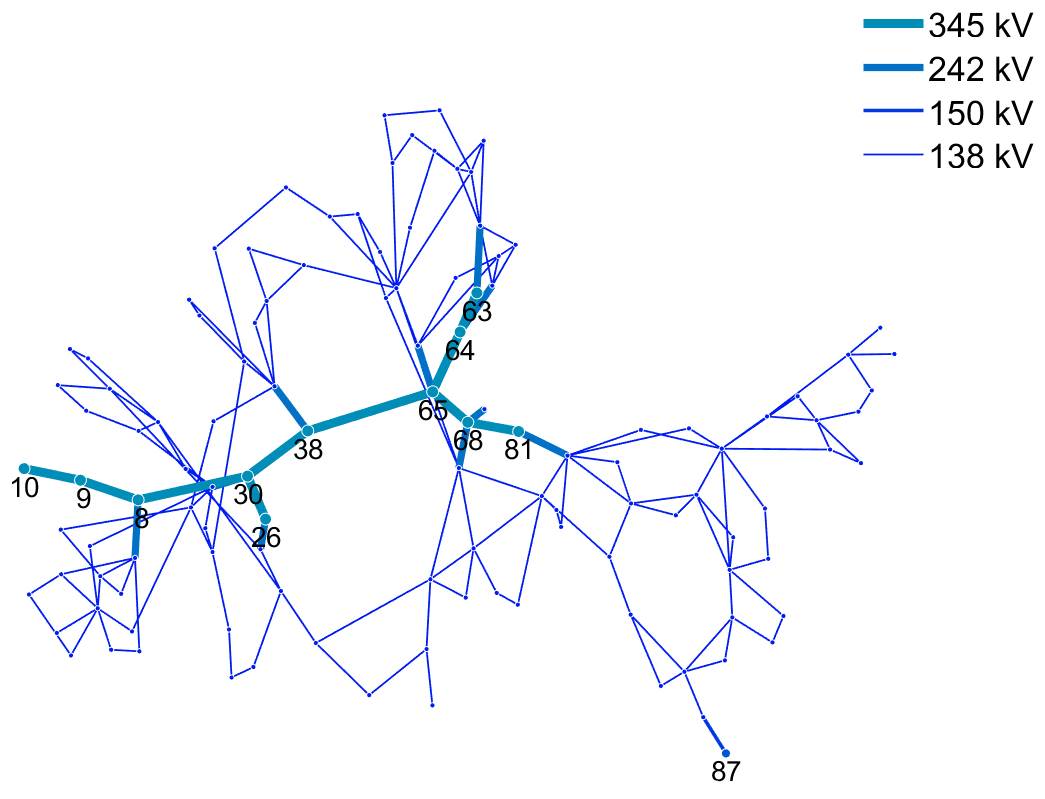
\includegraphics[scale=0.6]{immagini/118graph.png}
        \caption{ A modified IEEE 118-bus test system.}
        \label{fig:118busFig}
\end{figure}


The wind power forecast errors were obtained from a data source provided by CESI. The process involves fitting a Weibull distribution to represent the probability distribution of wind power production. The predicted power output is then set as the mean of this distribution. Error samples are generated by drawing random samples from the fitted distribution and then computing the discrepancy with the predicted power generation.

To align our findings with existing literature \cite{DBDRSOPF2}, we adjusted our forecasting errors to have a zero mean. Additionally, standard deviations were set at $200MW$ for wind farms \#1 and \#9, and $300MW$ for wind farm \#26. We focused on the single-period stochastic optimization problem following the approach in \cite{DBDRSOPF2}.
%we did not impose bounds on the wind power forecast errors, denoted as $\xi_{\tau}$. This choice reduces the model's complexity by eliminating the variable $\gamma_{tio}$ from \eqref{finite reduction in model}

The dataset comprises 152 observations and is divided into 13 samples to train the model and 139 test samples for measuring the out-of-sample performance of the solution. Therefore $N_s = 13$ and $N_{\Xi} = 3$ since there are three windfarms whose power generation is predicted. The optimization task was completed in 100 seconds for each loop on a laptop equipped with an Intel(R) Core(TM) i5-8250U CPU @ 1.60GHz 1.80 GHz and 8GB of RAM. 

\begin{figure}[ht]
    \centering
    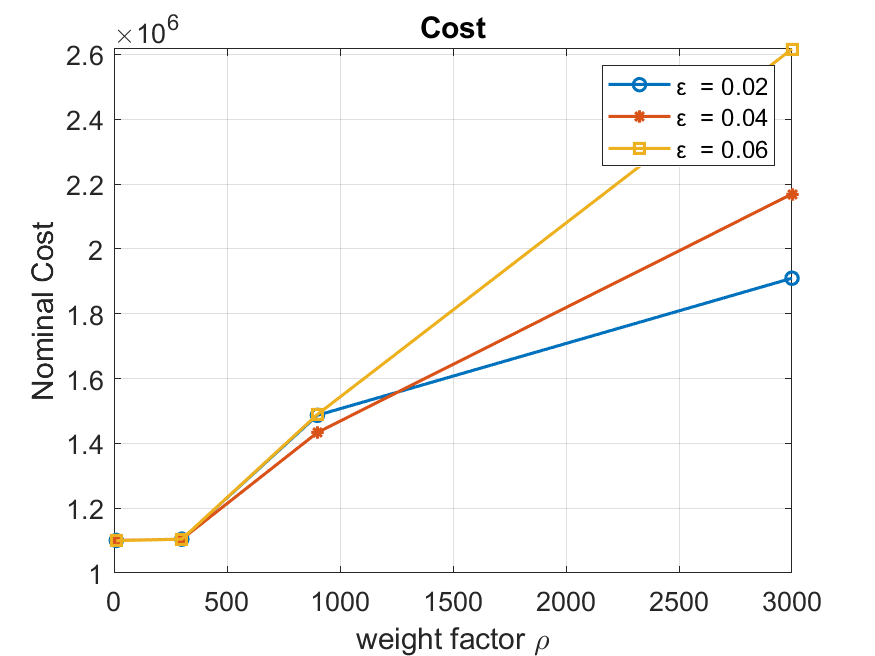
\includegraphics[scale=0.6]{immagini/AverageOpCost.png}
    \caption{Comparison of the average operational cost for various values of risk aversion $\rho$ and Wasserstein metric radius $\varepsilon$.}
    \label{AverageOPCost}
\end{figure}

\noindent
Figure \ref{AverageOPCost} illustrates the variation in the average operational cost based on different values of the risk aversion parameter \( \rho \) and the radius \( \varepsilon \) of the Wasserstein metric. An evident trend is the rise in average nominal cost as \( \rho \) increases. This indicates a greater focus on avoiding constraint violations across all potential realizations of \( \xi \). While this strategy ensures higher security, it does come at the cost of increased operational expenses.

\begin{adjustwidth}{-1.5cm}{-1.5cm}    
\begin{figure}[!ht]
    \centering
    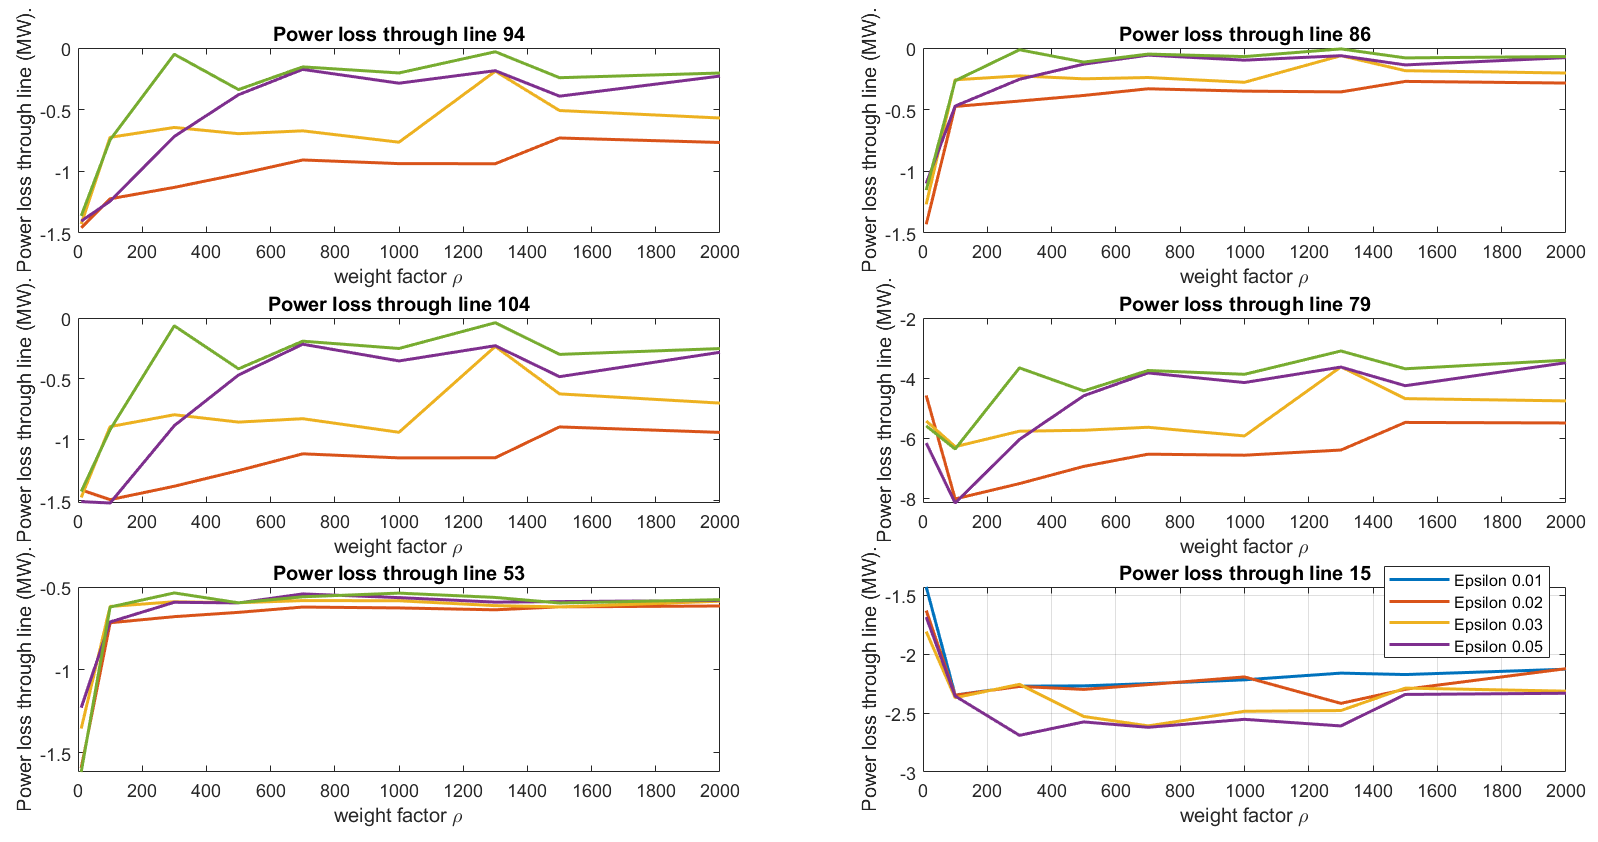
\includegraphics[scale=0.29]{immagini/PowerLossLines.png}
    \caption{Comparison of the power loss in six lines of the network for various values of risk aversion parameter $\rho$ and the Wasserstain metric radius $\varepsilon$.}
    \label{PowerLossLines}
\end{figure}
\end{adjustwidth}

\begin{figure}[!ht]
    \centering
    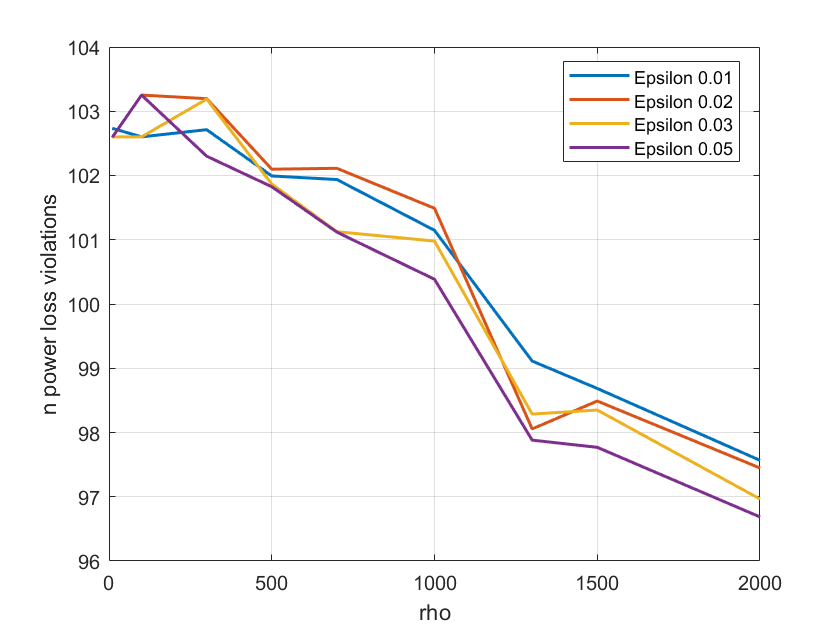
\includegraphics[scale=0.5]{immagini/NPloss.png}
    \caption{Comparison of the number of out of samples constraints violation for various values of risk aversion parameter $\rho$ and the Wasserstain metric radius $\varepsilon$.}
    \label{NPloss}
\end{figure}

\noindent
Figure \ref{PowerLossLines} showcases the nominal power loss in some key lines of the network, a discernible pattern is the decreasing constraint violation as \(\rho\) increases for all lines except for line 15. This happens because a overall lower cost is achieved by allowing higher risk of violating the power loss constraint in line 15.  In Figure \ref{NPloss}, we observe how out of sample performance varies with $\varepsilon$. In particular, \ref{NPloss} shows the average number of power loss constraint violations of the test samples. We observe that large $\varepsilon$ ensures fewer constraints violations. Inequality affine constraints on power generation and voltage magnitudes, implemented as policy constraints as described in Section \ref{Inequality affine constraints}, are never violated for the tests samples. 


Lastly,  Figure \ref{PowerOutput fig}  shows  the relationship between nominal real power output and the risk aversion coefficient \(\rho\). A discernible pattern is the increasing conservatism in policy as \(\rho\) elevates. This ensures respect for magnitude constraints, especially when confronted with extreme realizations of the predictions error \(\xi\). However the change in power generation in some buses, as in bus 15 and bus 31, is not monotonic. This due to the nonlinearities of the OPF model, which make the behavior of the solution with respect to the changes of various parameters somewhat impredictable.
 
% \textcolor{red}{forse le figure con tante linee / bus ne esporterei una alla volta per poterle piazzare nel latex con più facilità. se vogliamo proprio strafare si possono salvare i dati e far compilare le figure da tikz}


% \begin{figure}[ht]
%     \centering
%     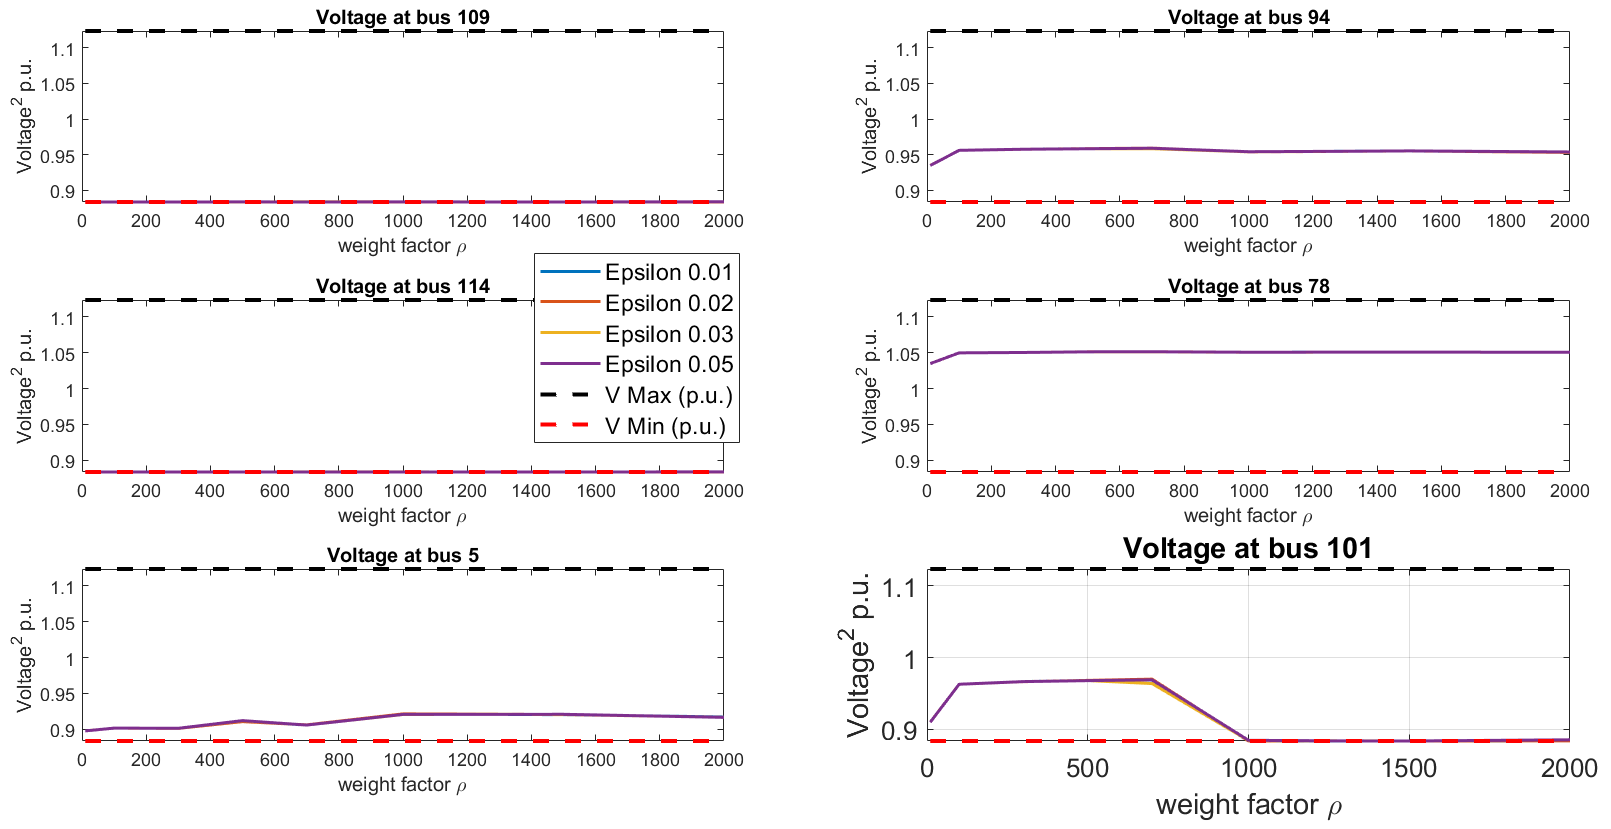
\includegraphics[scale=0.29]{immagini/Voltage.png}
%     \caption{Comparison of voltage of selected buses for various values of risk aversion $\rho$ and Wasserstein metric radius $\varepsilon$.}
%     \label{Voltage fig}
% \end{figure}


% \begin{figure}[!ht]
%     \centering
%     \includegraphics[scale=0.7]{immagini/CVar.png}
%     \caption{Comparison of the risk of constraint violation for various values of risk aversion parameter $\rho$ and the Wasserstain metric radius $\varepsilon$.}
%     \label{PowerOutput fig1}
% \end{figure}

\begin{figure}[!ht]
    \centering
    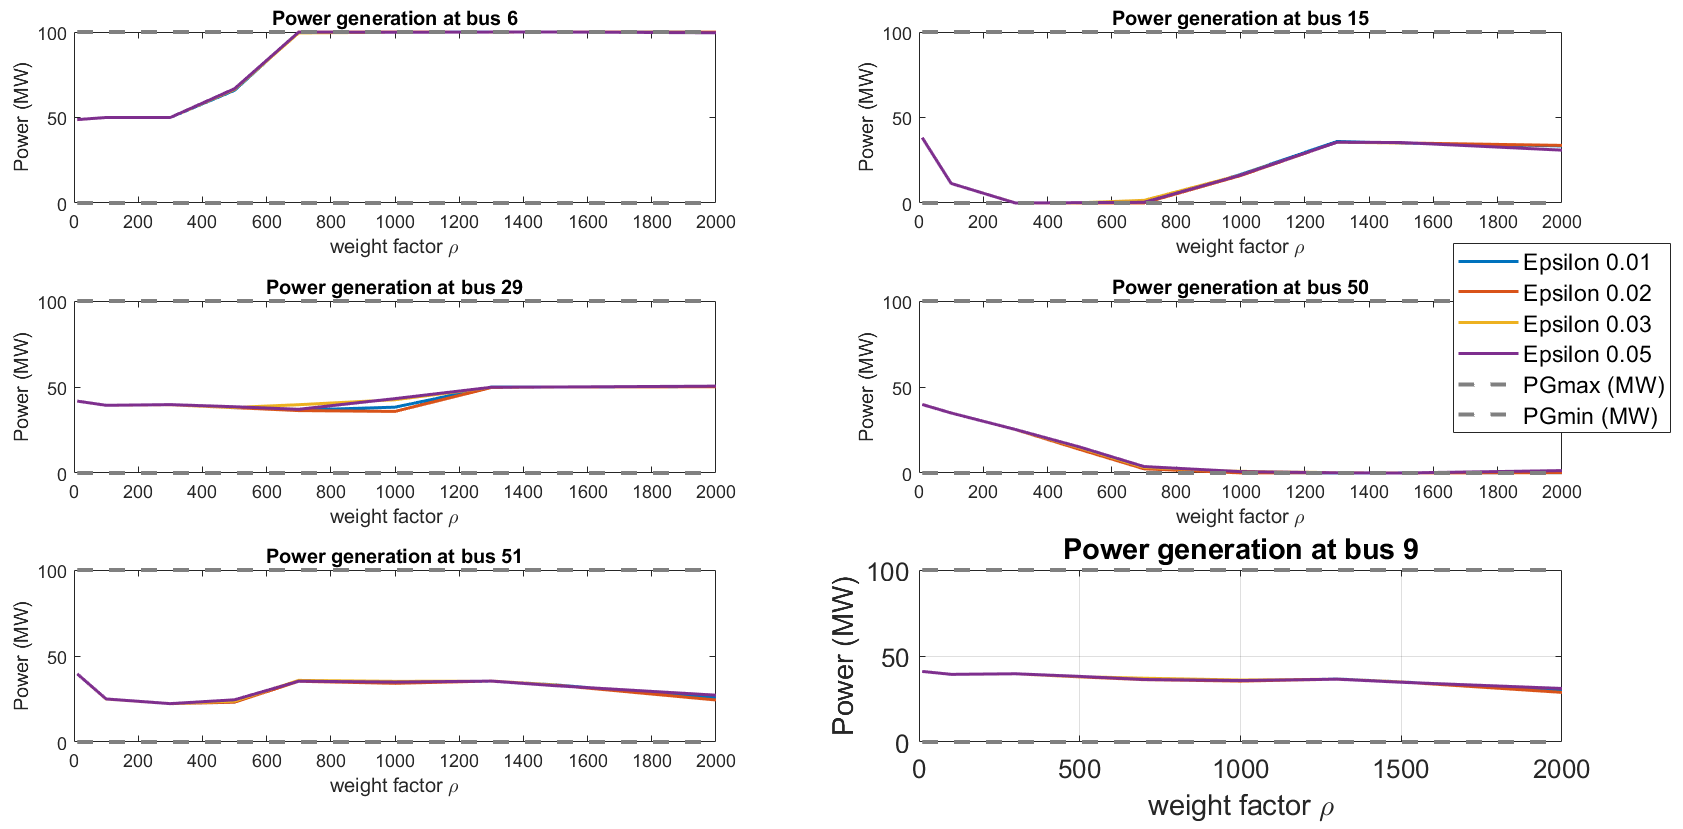
\includegraphics[scale=0.28]{immagini/RealPowerGen.png}
    \caption{Comparison of output real powers of selected generators for different risk levels $\rho$ and Wasserstein metric values $\varepsilon$.}
    \label{PowerOutput fig}
\end{figure}

\chapter{Conclusions}
We have showcased the efficacy and adaptability of our proposed data-driven, distributionally robust stochastic OPF methodology. Unlike many existing models, ours directly integrates error training datasets, eliminating the need to presuppose a forecast error distribution. This approach allows us to use distributionally robust optimization techniques, leading to enhanced out-of-sample performance. Importantly, our underlying deterministic model operates with fewer assumptions compared to the conventional DC OPF. This ensures resilience, especially when faced with extreme weather events or fluctuating demand scenarios in the network. We introduced a novel method of modeling affine inequality constraints as continuity constraints on the policy, allowing us to impose fewer constraints using Conditional Value at Risk (CVaR). The key distinction between these two approaches is that the former is 'hard,' enforcing the constraint for every possible realization of error predictions but is only applicable to affine constraints, while the latter can be applied more generally to concave constraints but it does not guarantee compliance for every possible realization of error predictions.
However, it is worth noting that our model tends to be more computationally demanding than the DCOPF-based stochastic optimal power flow model presented in \cite{DBDRSOPF2}, due to the increased number of variables and constraints derived from the AC OPF formulation.
To reduce the number of variables and constraints, one approach is to identify the critical lines in the network, by running a relaxation of the model without the line constraints and by identifying where these constraints are violated, and apply the CVaR constraints exclusively to these lines. From simulations results, we observed that larger \(\varepsilon\) may lead to large constraint violation when the sum of the CVars has a lower overall risk by allowing higher risk of violation of specific constraints. This may addressed by considering the risk of joint constraint violation instead of modeling each constraint individually. In our model we considered $\Xi$ to be in the form $[-E_1,E_1]\times [-E_2,E_2] \times [-E_3,E_3]$. Although this would work well if the components of $\xi$ were independent, this is rarely the case for wind power prediction, and this results in overly conservative policies. Therefore a better approach, could be to consider the best polytope fitting the considered samples. Moreover, limiting our consideration to affine policies in a nonlinear problem like the OPF overlooks numerous admissible policies that are nonlinear but have the potential to be more optimal. A potential avenue for future research could involve exploring piecewise affine policies instead.


\par In Chapter \ref{Graph results chapter}, we integrated the loop constraints \ref{loop constraint} into the Jabr model \eqref{Jabr equality model}. This integration aimed at achieving exactness in non-radial networks. These constraints are in general non convex but a linear relaxation of these constraints can be implemented by using McCormick envelops. Furthermore, the calculation of the loop constraint becomes increasingly difficult with the length of the loop. Since there is not a unique Cycle Base, this could be addressed by choosing the Cycle Base with the smaller maximum length of the cycles in the Cycle Base. This is similar to the minimum weight cycle base problem \cite{CycleBasesInGraphs}.
Proposition \ref{prop: loop constraints solution} offers a parametrization of the solution space of the loop constraints, the behavior of this parametrization in conjunction with the other constraints of the OPF problem remains uncertain. A promising avenue for future research would be to discern the conditions under which the image of this parametrization is included in or equals to the solution space of the OPF problem \ref{polar}.

%  Following the approach in \cite{DBDRSOPF2}, in Section \ref{Numerical results} we did not impose bounds on the wind power forecast errors, denoted as $\xi_{\tau}$, that is we considered the whole ambiguity $\Xi$ to span over all $\bR^{N_{\xi}}$. However in this section we explore potential benefits of treating the set $\Xi$ as a compact polytope. Given the finite nature of eolic energy production and the subsequent error bounds on its prediction, it would be pragmatic to assume \(\Xi\) as limited. The first immediate benefit of this assumption is that it would make the obtained eventually obtained policies more conservative, because  the ambiguity set $\cB_{\varepsilon}(\hat \bP_N)$ would not include unrealistic extreme distributions (for example where the error on the prediction is greater than the maximum possible production of eolic generators). Further more if the polytope $\Xi \coloneqq \{ y \in \bR^{N_{\xi}} \mid Hy \leq d\}$ has $0 \in \bR^{N_{\xi}}$ as a simmetry point and the matrix \(H \in \bR{2N_{\xi} \times N_{\xi}}\) is of full rank then considering affine inequality constraints in \(\ref{Jabr concave relaxation}\), in the form 
%  \begin{equation} \label{voltage like constraint}
%  m \leq A(\pi)\xi + b(\pi) \leq M \; \forall \xi \in \Xi
% \end{equation}
%  where $m \leq b(\pi) \leq M$ we can impose these as constraints on the policy instead of considering the risk of constraint violation with the conditional value at risk CVar, thus reducing the number of variables in the model.

%  If equation \ref{voltage like constraint}, 
% \[-M - b(\pi) \leq A(\pi)\xi \leq M + b(\pi)\] 
% must hold for all \(\xi \in \Xi\), then define
% \[ r \coloneqq \min\{\|-m - b(\pi)\|, \|M + b(\pi)\|\} \]
% such that \( A(\pi)\xi \in B_r(0)\) if and only if \ref{voltage like constraint} holds since $0$ is a simmetry point of $\Xi$. Moreover, if \(H\) has dimensions \( 2N_{xi} \times N_{xi}\) and is of full rank, then a linear isomorphism \( L: \mathbb{R}^{N_{xi}} \to \mathbb{R}^{N_{xi}}\) exists such that \(L(\Xi)\) corresponds to the \(\|\|_1\)-norm ball, (i.e. a cube). Thus $A(\pi)\xi \in \B_r(0) \; \forall \xi \in \Xi$ if and only if $A(\pi)Lx \in \B_r(0) \; \forall x \in B^{\|\cdot\|_1}_r(0) $. This is true if and only if the linear function $A(\pi)L: (\bR^{N_{xi}},\|\cdot\|_1 \la \bR$ has continuity norm less or equal than $r$. So the constrain \ref{voltage like constraint} is equivalent to:
% \begin{equation}
%     \|A(\pi)L\|_{\infty} \leq r = \min\{\|-m - b(\pi)\|, \|M + b(\pi)\|\}
% \end{equation}
% which can be written as finite number of finite constraints on the policy $\pi$.
% In particular this could be applied to the constraint on the voltage and power generation magnitutes. Policies would be more conservative with values of $b$ (nominal value) closer to the limit of the constraint, so as not to violate it, and less so when the nominal value is centered.


% \begin{figure}[h]
%     \label{AverageOPCost}
%     %\hspace*{-2cm} % Adjust this value as needed to shift the image to the left
%     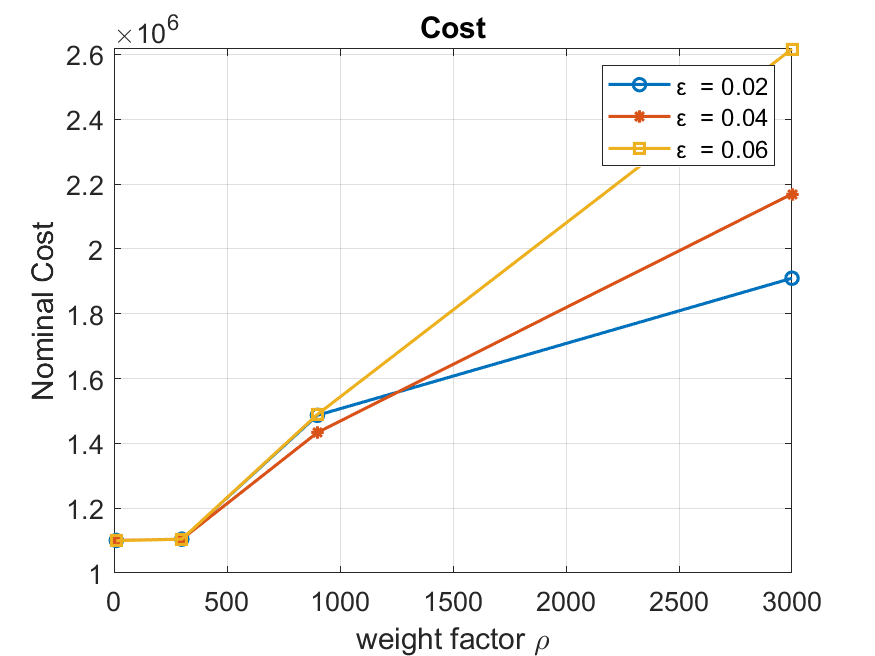
\includegraphics[scale=0.5]{immagini/AverageOpCost.png}
%     \centering
%     \caption{Comparison of the average operational cost for various values of risk aversion $\rho$ and Wasserstein metric radius $\varepsilon$.}
% \end{figure}

% Figure \ref{AverageOPCost} illustrates the variation in the average operational cost for different values of the risk parameter \( \rho \) and the radius of the Wasserstein metric \( \varepsilon \). As \( \rho \) increases, we notice a consistent rise in the average nominal cost. This is attributed to placing a heightened emphasis on ensuring constraints are not violated for all potential realizations of \( \xi \). While this approach enhances the security against constraint violations, it also escalates operational costs.

% \begin{figure}[h]
%     \label{Voltage fig}
%     \hspace*{-2cm} % Adjust this value as needed to shift the image to the left
%     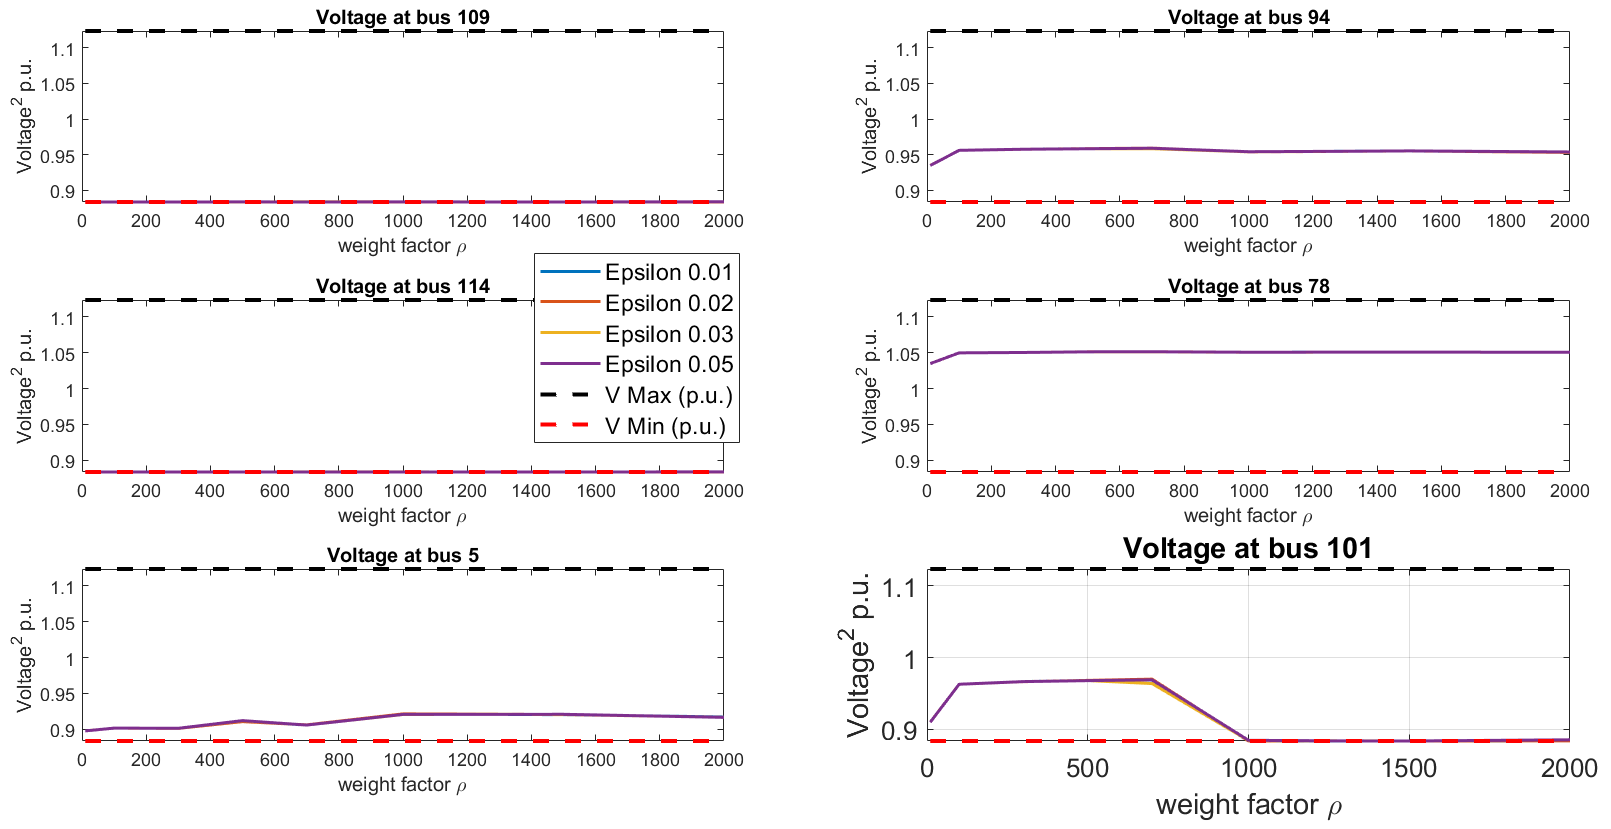
\includegraphics[scale=0.3]{immagini/Voltage.png}
%     \centering
%     \caption{Comparison of voltage of selected buses for various values of risk aversion $\rho$ and Wasserstein metric radius $\varepsilon$.}
% \end{figure}

% Figure \ref{Voltage fig} displays the comparison of voltage magnitudes at randomly selected buses within the electrical network. As \(\rho\) increases, the adopted policy becomes more conservative, ensuring that the magnitude constraints are respected even in the face of more extreme realizations of the power generation error \(\xi\). The same fenomenon can be observed in Figure \ref{PowerOutput fig} comparing between real power output generation  and the risk aversion parameter $\rho$.


% \begin{figure}[h!]
%     \label{PowerOutput fig}
%     \hspace*{-2cm} % Adjust this value as needed to shift the image to the left
%     \includegraphics[scale=0.3]{immagini/CVar.png}
%     \centering
%     \caption{Comparison of output real powers of selected generators for various values of risk $\rho$ and Wasserstein metric $\varepsilon$}
% \end{figure}


% \begin{figure}[h!]
%     \label{PowerOutput fig}
%     \hspace*{-2cm} % Adjust this value as needed to shift the image to the left
%     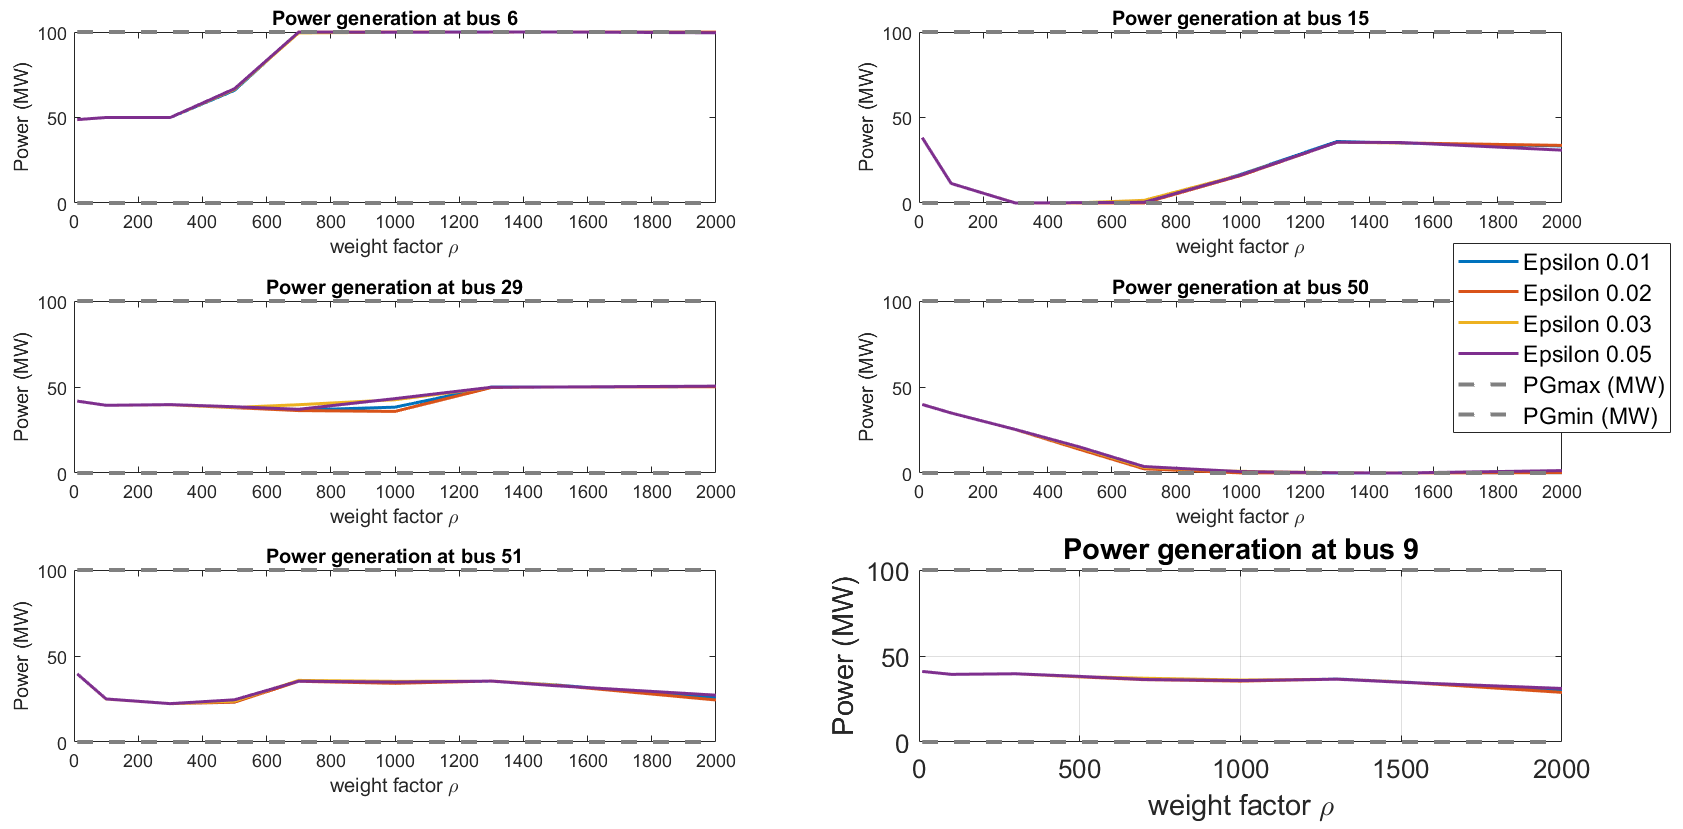
\includegraphics[scale=0.3]{immagini/RealPowerGen.png}
%     \centering
%     \caption{Comparison of output real powers of selected generators for various values of risk $\rho$ and Wasserstein metric $\varepsilon$}
% \end{figure}







\backmatter


\begin{footnotesize}


\printbibliography[
heading=bibintoc,
title={Bibliography}]



\end{footnotesize}
\pagebreak
\vspace*{1.5cm}
\begin{flushright}
\begin{minipage}{.9\textwidth}
\chapter*{}
{\bf \huge Acknowledgements} \vspace{20 pt} \\
This thesis began as I contemplated the question, "What can a mathematician do in the face of a dying tree?". I believe sincerely that the most honest answer to this is: "go protest and vote well". Still, this thesis represents my initial step towards understanding what I, as both an individual and a mathematician, can do to contribute to the fight against climate change. This problem, as many others, cannot be tackled alone, and the same holds true for this thesis: It wouldn't have materialized without the invaluable support of many individuals.

I would like to extend my heartfelt gratitude to my advisor, Stefano Gualandi, who responded to the aforementioned question with a practical offer: "I'm working on this project; would you like to be involved?". I am immensely thankful to Stefano Gualandi and Ambrogio Bernardelli for their unwavering guidance, infinite patience, and the substantial amount of time they generously devoted to discussing ideas.

Thanks to all the people who were part of the Tesanza this summer: Francesca, Bianca, Marcello, Eleonora and my parents. Thank you for always creating such a cozy environment, just by being there. Thanks Francesca for the unwavering potato and to Ino, Illo, Ito, Etotito, Rni, and all the others we still have to discover. Thanks to my (self-adopted) sister, Alessia, for sharing struggles, music and adventures with me. Thanks to my brother (not adopted), Marco, and all the other members of the SIS: Tosca, Violetta, Marta R., Giulia and Matteo. For the science, the space, the laughs and the food. The time spent together was fundamental to putting together all the pieces and writing this thesis, but most of all, it was really fun. Thanks to Marta P., Elisa and Ambrogio, your friendship will always be dear to me. And to the new friends: Thank you Tessa for reminding me that friendship can just, kind of happen.
And thank you Vale for the cheese cake, it was really good.

\begin{footnotesize}


\end{footnotesize}
\end{minipage}

\end{flushright}







%\end{justify}





\end{document}
